% =============================================================================
% Indirect reciprocity with inertial reputation updating
% Integrated manuscript draft (main text, Methods, Extended Data and
% Supplementary Information), 3 November 2026.
%
% Sources (all in Manuscript_doc/):
%   Introduction_V2.docx      -> Introduction (version 2, light edits only)
%   Results_Outline.docx      -> Results, figure and Extended Data legends
%   Methods.pdf               -> Methods (equations shown in the Results are
%                                referenced rather than repeated)
%   Supplementary_Information.pdf -> Supplementary Information (content kept;
%                                Extended Data numbers updated to the figure files)
%   Fig1_model.pdf, Fig2-5.pdf, ED_Fig1-9.pdf -> figures (read from ../)
%
% Build:  pdflatex -> bibtex <jobname> -> bibtex SI -> pdflatex -> pdflatex
%         (latexmk -pdf also works). The second bibtex run builds the
%         separate Supplementary reference list (multibib).
%
% Draft notes are printed in dark red. Set \draftnotesfalse to hide them.
% =============================================================================
\documentclass[fleqn,10pt]{wlscirep}
\usepackage[T1]{fontenc}
\usepackage{amsthm,bm,mathrsfs,array,longtable}
\usepackage[resetlabels]{multibib}
\newcites{SI}{Supplementary References}

\graphicspath{{../}}
% Journal names are already abbreviated (Nature style) in references.bib.
\renewcommand{\JournalTitle}[1]{#1}
\setlength{\emergencystretch}{2em}
\allowdisplaybreaks
\def\UrlBreaks{\do\/\do\_\do-}

% ---------------------------------------------------------------- draft notes
\newif\ifdraftnotes
\draftnotestrue
\DeclareRobustCommand{\draftnote}[1]{%
  \ifdraftnotes{\color{red!60!black}\sffamily\footnotesize[#1]}\fi}

% ------------------------------------------------------------------- notation
\newcommand{\Rmap}{\mathscr{R}}            % reputation map
\newcommand{\Lspace}{\mathscr{L}}          % latent state space
\newcommand{\st}[1]{\mathrm{#1}}           % latent states G, B, W_m, S_n
\newcommand{\Pp}[1]{P^{+}_{\mathrm{#1}}}   % e.g. \Pp{C|G}
\newcommand{\rR}{r_{\mathrm{R}}^{*}}
\newcommand{\uR}{u_{\mathrm{R}}^{*}}
\newcommand{\rX}{r_{\mathrm{X}}^{*}}
\newcommand{\uX}{u_{\mathrm{X}}}
\newcommand{\PhiC}{\Phi_{\mathrm{C}}}
\newcommand{\PhiD}{\Phi_{\mathrm{D}}}
\newcommand{\dPhi}{\Delta\Phi^{*}}
\newcommand{\Hmin}{H_{\min}}
\newcommand{\dd}{\mathrm{d}}
\newcommand{\ALLC}{\mathrm{ALLC}}
\newcommand{\ALLD}{\mathrm{ALLD}}
\newcommand{\DISC}{\mathrm{DISC}}

% ------------------------------------------- statements (used in the SI only)
\theoremstyle{plain}
\newtheorem{lemma}{Lemma}
\newtheorem{proposition}[lemma]{Proposition}
\newtheorem{corollary}[lemma]{Corollary}
\renewcommand{\thelemma}{S\arabic{lemma}}

% -------------------------------------------------------------------- figures
\newcommand{\figfile}[2][0.66]{%
  \includegraphics[width=\linewidth,height=#1\textheight,keepaspectratio]{#2}}

% ---------------------------------------------------------------- front matter
\title{Indirect reciprocity with inertial reputation updating}

\author[1,2]{Wenqiang Zhu}
\affil[1]{School of Artificial Intelligence, Beihang University, Beijing 100191, China}
\affil[2]{Key Laboratory of Mathematics, Informatics and Behavioral Semantics, Beihang University, Beijing 100191, China}
\affil[ ]{\textit{Complete author list, affiliations and correspondence details to be added.}}

\begin{abstract}
\draftnote{Temporary abstract, to be revised.}
Indirect reciprocity can sustain cooperation among strangers when individuals help those with a good reputation. When reputations are formed privately from noisy observations, however, observers often disagree, and a single assessment can overturn an established reputation. Here we introduce inertial reputation updating, in which evidence against good standing and evidence for recovery from bad standing accumulate along separate paths, and in which intermediate states can already affect how individuals are treated. Combining individual-based simulations with a mean-field theory of private assessment, we show that the allocation of inertia between the two paths determines whether private reputations are both shared and discriminating. Compact, norm-specific architectures, selected on these reputational criteria alone, support highly cooperative outcomes under four classical norms and enlarge their basins of attraction. Cooperation depends on how inertia is allocated rather than on its total amount. Tolerance of negative evidence can, however, allow occasional defectors to invade even when unconditional defectors are excluded. Letting warning states carry partial social consequences excludes the opportunistic strategies we test while preserving high cooperation.
\end{abstract}

\begin{document}
\raggedbottom
\maketitle

% =============================================================================
\section*{Introduction}
% Source: Introduction_V2.docx. Edits: two colons replaced by full stops
% (paragraphs 3 and 6); "Importantly, ..." sentence split; citations mapped
% to references.bib in the original order (refs 1-42).

Reputation allows past behavior to shape future social opportunities.\cite{milinski2016} Individuals who are known to help others are more likely to receive help themselves, enabling cooperation even when partners do not repeatedly interact.\cite{nowak1998,wedekind2000,milinski2002} This principle underlies indirect reciprocity, a prominent explanation for cooperation among unrelated individuals\cite{nowak2005} and a theoretical framework for studying how social norms turn observed behavior into moral standing.\cite{ohtsuki2004,santos2018,kessinger2023,murase2024computational} Classical analyses have identified social norms capable of sustaining high levels of cooperation,\cite{leimar2001,panchanathan2003,ohtsuki2006} but their success depends on reputation information being public, so that observers agree on each other's social standing. In real social environments, information is instead noisy and privately interpreted.\cite{takahashi2006,uchida2010} Observers can then disagree about who is good, and such disagreements can undermine the very cooperation that reputations are meant to support.\cite{hilbe2018,okada2018,fujimoto2023,murase2024synchronization}

Private assessment exposes a fundamental fragility of standard reputation models. A donor and an observer may hold different opinions of the same recipient and therefore disagree over whether the donor's action was justified.\cite{hilbe2018,radzvilavicius2019,okada2020} Moreover, in the conventional binary framework, each new assessment immediately replaces an existing good or bad image.\cite{ohtsuki2004} A single mistaken or conflicting observation may therefore undo a reputation built over many previous interactions. Recent work has developed several ways to make reputation systems more robust. Some mechanisms restore agreement among observers, through public institutions,\cite{radzvilavicius2021} gossip,\cite{kawakatsu2024} empathetic evaluation\cite{radzvilavicius2019} or the synchronization of private opinions.\cite{murase2024synchronization,tham2026,okada2024} Others change how individuals assess and integrate information: generous or stochastic assessment rules,\cite{schmid2021,murase2023} graded reputations,\cite{tanabe2013,murase2022} reasoning about errors,\cite{pandula2024,morsky2024} quantitative scores that accumulate evidence rather than binary labels,\cite{schmid2023,clark2020} and the aggregation of multiple observations before a reputation is assigned.\cite{michelmata2024} These approaches demonstrate that using social information beyond the latest isolated observation can substantially improve reputation-based cooperation.

Yet a general question remains unresolved: how should a reputation system integrate behavioral evidence over time? Accumulating information is not equivalent to simply using more of it. An established good reputation may persist while evidence against it accumulates, and recovery from a bad reputation may follow a different process. Existing approaches, however, typically treat losing and regaining standing as a single process governed by one score, threshold or observation window.\cite{schmid2023,michelmata2024,yamamoto2025} Human social evaluation is dynamic and directional. People revise impressions in response to sequences of behavior,\cite{yamamoto2025,mendesiedlecki2013neural} evidence differs in its diagnostic impact on existing beliefs,\cite{reeder1979,skowronski1989,mendesiedlecki2013diagnostic} and beliefs about good and bad individuals are updated asymmetrically.\cite{siegel2018} Social institutions follow a similar logic. Shared resources are often governed by graduated sanctions that escalate with repeated violations,\cite{ostrom1990,cox2010} and restoring one's standing after a criminal record takes years.\cite{blumstein2009} These observations motivate reputation mechanisms in which standing has inertia, and in which the inertia of losing standing can differ from that of regaining it.

Here we introduce a directional framework for inertial reputation updating. Instead of allowing every assessment to overwrite the current image, contrary evidence moves an individual through intermediate reputation states (Fig.~\ref{fig:model}). Evidence for losing good standing and evidence for recovering it accumulate along separate paths, allowing the two processes to have different depths. Each intermediate state is in turn read as good or bad with a specified probability, which determines how it is expressed in current social interactions. The framework therefore separates evidence accumulation, which determines when an established reputation changes, from evidence interpretation, which determines when incomplete evidence already affects treatment.

We first show that the allocation of inertia determines whether private reputations are both accurate and shared. Depending on how inertia is allocated, observers can become more accurate and consistent, or can agree while failing to distinguish cooperative from defective strategies. Compact, norm-specific architectures, selected solely by these reputational criteria and without reference to evolutionary outcomes, subsequently support highly cooperative evolutionary outcomes across Scoring, Shunning, Stern Judging and Simple Standing, and enlarge the basins of attraction of cooperative states. Importantly, these effects cannot be reduced to the total amount of memory. Allocations with the same depth can lead to sharply different evolutionary outcomes, and increasing depth does not necessarily increase cooperation.

Finally, we identify a limit to reputational tolerance. A mechanism that protects individuals from isolated negative assessments can also protect those who deliberately defect on occasion.\cite{schmid2021,michelmata2024} Excluding unconditional defectors therefore does not guarantee resistance to weaker opportunistic strategies. In our framework, this vulnerability can be controlled without changing how evidence is accumulated. Allowing warning states to affect current treatment restores a reputational cost to partial defection and, for the opportunistic strategies we test, creates a range of readouts in which opportunistic invasion is prevented while resident cooperation remains high. Together, these results show that reputation-based cooperation depends not only on which behaviors societies reward or punish, but also on how much evidence is required before reputations change and how emerging evidence is translated into social consequences.

% =============================================================================
\section*{Results}

\subsection*{A framework for inertial reputation updating}

We study indirect reciprocity in a well-mixed population in which randomly matched donors and recipients play the donation game. A donor can help a recipient at a cost $c$, conferring a benefit $b>c$. Unconditional cooperators (ALLC) always intend to cooperate, unconditional defectors (ALLD) always intend to defect, and discriminators (DISC) intend to cooperate only with recipients that they privately regard as good. Reputations are private. Each observer keeps its own record of every individual and assesses a donor's realized action by applying a social norm to its own image of the recipient.\cite{hilbe2018,okada2018} We consider four second-order norms,\cite{ohtsuki2004} Scoring (SC), Shunning (SH), Stern Judging (SJ) and Simple Standing (SS). They agree that helping a recipient regarded as good deserves a positive assessment and that refusing such help deserves a negative one. They differ in how they judge actions towards recipients regarded as bad. Assessments are noisy. Intended cooperation fails with probability $e_1$ (implementation error), and an observer records the opposite assessment with probability $e_2$ (assessment error; Methods).

Under instantaneous updating, the latest assessment replaces the previous binary image (Fig.~\ref{fig:model}a). Under inertial updating, each observer instead keeps an internal record of every individual (Fig.~\ref{fig:model}b). Consecutive negative assessments move an individual in good standing through $k_1$ warning states, $\st W_1,\ldots,\st W_{k_1}$, before the record becomes bad. Consecutive positive assessments move an individual in bad standing through $k_2$ recovery states, $\st S_1,\ldots,\st S_{k_2}$, before the record becomes good. An assessment that supports the established judgment resets the record to the corresponding established state. Losing good standing therefore requires $k_1+1$ consecutive negative assessments, and regaining it requires $k_2+1$ consecutive positive assessments, by the same observer about the same individual. We call $k_1$ the tolerance depth, $k_2$ the strictness depth and $K=k_1+k_2$ the total depth. The two depths are set independently, so losing and regaining standing need not be equally fast. The pair $(k_1,k_2)=(0,0)$ recovers instantaneous updating, and $(k_1,k_2)=(1,1)$ defines one-step inertia.

\begin{figure}[tbp]
\centering
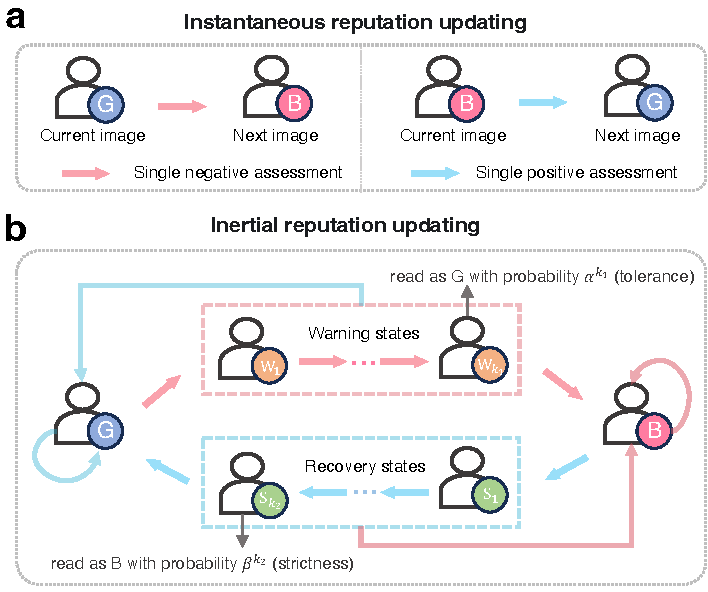
\includegraphics[width=0.68\linewidth]{Fig1_model}
\caption{\textbf{A framework for inertial reputation updating.}
\textbf{a}, Under instantaneous updating, a single negative or positive assessment replaces the current binary image.
\textbf{b}, Under inertial updating, negative assessments move a good record through warning states $\st W_1,\ldots,\st W_{k_1}$ towards bad, whereas positive assessments move a bad record through recovery states $\st S_1,\ldots,\st S_{k_2}$ towards good. An assessment in the opposite direction resets the record to the corresponding established state. The tolerance depth $k_1$ and the strictness depth $k_2$ are set independently. Warning state $\st W_m$ is read as good with probability $\alpha^m$ (tolerance strength $\alpha$), and recovery state $\st S_n$ is read as bad with probability $\beta^n$ (strictness strength $\beta$). The diagram labels these probabilities for the final state of each path. Pink and blue arrows denote negative and positive assessments, respectively.}
\label{fig:model}
\end{figure}

The internal record is distinct from the binary image used in interactions. Whenever a record is consulted, either to choose an action or to assess someone else's action, it is read as good or bad. Warning state $\st W_m$ is read as good with probability $\alpha^m$, and recovery state $\st S_n$ is read as bad with probability $\beta^n$. We call $\alpha$ the tolerance strength and $\beta$ the strictness strength. Under full readout, $\alpha=\beta=1$, an established image persists until the relevant path is completed. With $\alpha<1$ or $\beta<1$, incomplete evidence already affects current treatment. The depths therefore determine how much consistent evidence is needed to reverse an established reputation, whereas the strengths determine how strongly incomplete evidence is expressed before that point. Throughout, we compare instantaneous updating (no inertia), full one-step inertia ($k_1=k_2=1$ with $\alpha=\beta=1$) and norm-specific multi-step architectures with full readout, which are introduced below. We first ask how this temporal integration of behavioral evidence changes reputation formation itself.

% -----------------------------------------------------------------------------
\subsection*{Directional inertia shapes private reputation dynamics}

We first examined reputation formation in finite populations containing equal numbers of ALLC, ALLD and DISC individuals. Each DISC observer keeps a separate record of every individual, and strategies do not change (Methods). Without inertia, each norm fails in a characteristic way (Fig.~\ref{fig:recognition}a--d, top row). Under SC, ALLC is regarded as good and ALLD as bad, but observers are divided about discriminators. SH drives almost every reputation towards bad. SJ sustains widespread disagreement, and SS extends substantial trust to defectors. Full one-step inertia does not resolve these failures uniformly (Fig.~\ref{fig:recognition}a--d, middle row). Under SH, observers agree largely because nearly everyone is judged bad. Under SJ, they retain extensive disagreement. Agreement alone is therefore insufficient. We measure recognition by the reputational separation $\Delta g=(g_{\DISC}+g_{\ALLC})/2-g_{\ALLD}$, where $g_I$ is the probability that a randomly chosen DISC observer regards a randomly chosen type-$I$ individual as good. We measure agreement by the mean disagreement $\bar d$, the probability that two DISC observers hold different images of the same individual, averaged over individuals (Methods). Together, these quantities indicate whether cooperative and defective strategies receive distinct reputations and whether observers agree about individual targets.

Allocations with the same total depth can produce markedly different separation and disagreement (Fig.~\ref{fig:recognition}e--h). We used $\Delta g\geq0.8$ and $\bar d\leq0.1$ as operational criteria and selected the qualifying depth pair with the smallest total depth. This gives $(k_1,k_2)=(2,0)$ for SC, $(3,0)$ for SH, $(4,3)$ for SJ and $(1,2)$ for SS. Meeting both criteria thus requires depth on the path that protects good standing under SC and SH, depth on both paths under SJ, and a relatively longer recovery path under SS. In 30 independent replicate simulations, these architectures give separations between $0.88$ and $0.92$ and mean disagreement between $0.06$ and $0.08$ (Extended Data Fig.~\ref{ed:selection}a--d and Supplementary Table~\ref{tab:si-selected}). Their image matrices show good reputations for DISC and ALLC, bad reputations for ALLD and substantial agreement among observers (Fig.~\ref{fig:recognition}a--d, bottom row). The exact depth pairs depend on the chosen thresholds, whereas the directional patterns persist across a range of thresholds (Extended Data Fig.~\ref{ed:selection}e--h). We carry these four selected multi-step architectures forward. They were selected from reputation statistics alone, not from evolutionary outcomes.

\begin{figure}[tbp]
\centering
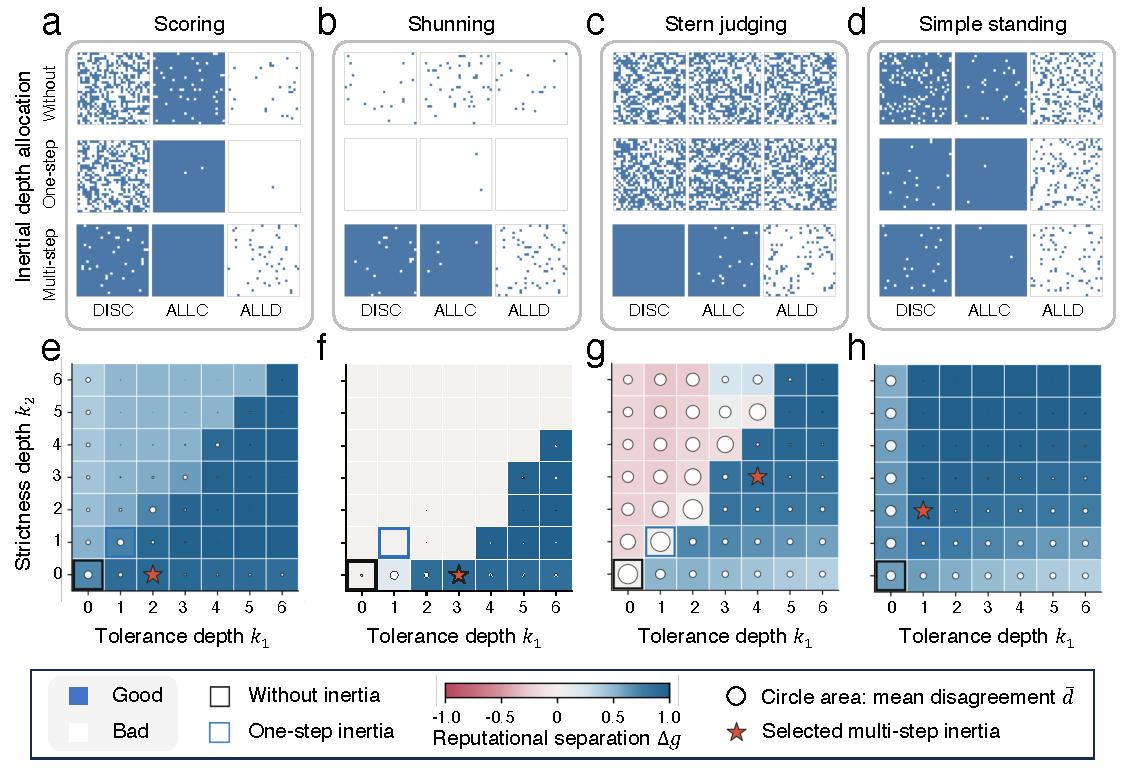
\includegraphics[width=\linewidth]{Fig2}
\caption{\textbf{The allocation of inertia shapes private agreement and strategy recognition.}
\textbf{a--d}, Illustrative private-reputation matrices under Scoring (SC; \textbf{a}), Shunning (SH; \textbf{b}), Stern Judging (SJ; \textbf{c}) and Simple Standing (SS; \textbf{d}). Panel rows show instantaneous updating (without inertia), full one-step inertia and the selected multi-step architectures. Within each matrix, rows are DISC observers and columns are DISC, ALLC and ALLD targets. Blue and white indicate good and bad images. Each matrix shows the final state of a single run.
\textbf{e--h}, Separation $\Delta g$ (color) and mean observer disagreement $\bar d$ (circle area) across tolerance depth $k_1$ and strictness depth $k_2$. Black and blue outlines mark instantaneous updating $(0,0)$ and one-step inertia $(1,1)$, respectively. Stars mark the pairs with the smallest total depth $K$ that satisfy $\Delta g\geq0.8$ and $\bar d\leq0.1$.
Parameters: $e_1=e_2=0.02$, equal proportions of the three strategies, population size $N=90$ for the matrices and $N=150$ for the depth scans (one run per condition), and $\alpha=\beta=1$ in the depth scans.}
\label{fig:recognition}
\end{figure}

Inertia also changes the reputation dynamics of a homogeneous DISC population (Extended Data Fig.~\ref{ed:resident}a--d). With full one-step inertia, SC, SH and SJ each exhibit bistability between high- and low-reputation stationary states. The reputation that a discriminator population reaches therefore depends on its reputational history. Under the selected multi-step architectures, this bistability disappears and the population has a single, high-reputation stationary state. Scans over the strengths $\alpha$ and $\beta$ and over the depths $k_1$ and $k_2$ show that both the reputation level and the presence of bistability depend on the norm and on the direction and strength of inertia (Extended Data Fig.~\ref{ed:reputation-planes}). The direction in which evidence accumulates therefore determines whether cooperative and defective strategies acquire distinguishable and consistent private reputations. Having shown that directional inertia can achieve both recognition and agreement, we next examine whether these reputations allow cooperation to emerge and persist as strategies evolve.

% -----------------------------------------------------------------------------
\subsection*{Directional inertia reshapes strategy dynamics}

We let the frequencies of ALLC, ALLD and DISC evolve under the replicator dynamics,\cite{hofbauer1998} assuming that reputations equilibrate quickly relative to strategy change. At each strategy composition, payoffs are computed from the stationary private reputations reached from initially good records, using a mean-field theory of private assessment (Methods). We report two measures of cooperation. Intended cooperation is the probability that a donor intends to help, evaluated at individual equilibria. The mean realized cooperation $\bar\rho$ is the long-run cooperation level averaged over initial strategy compositions sampled uniformly from the simplex. Figure~\ref{fig:dynamics}a shows the instantaneous baseline. SH and SJ do not support a cooperative evolutionary outcome. SC and SS can support cooperative configurations, but under neither norm is a pure DISC population a stable cooperative attractor.

Full one-step inertia makes a highly cooperative pure-DISC population locally stable under all four norms (Fig.~\ref{fig:dynamics}b). The basins of attraction of these cooperative states nevertheless remain narrow under SH and SJ. Only $8\%$ and $23\%$ of initial compositions, respectively, lead to cooperation.

The selected multi-step architectures enlarge the cooperative basins further (Fig.~\ref{fig:dynamics}c). Under SC, SH and SJ, pure DISC remains a stable cooperative attractor and is reached from $88\%$, $71\%$ and $71\%$ of initial compositions, respectively. Under SS, the cooperative attractor is a stable ALLC--DISC mixture, reached from $76\%$ of initial compositions. Across the four norms, these attractors reach near-complete intended cooperation (at least $99.99\%$) despite errors and private disagreement. Mean realized cooperation rises from $0.61$ without inertia to $0.87$ under SC, from $0$ to $0.69$ under SH, from $0$ to $0.70$ under SJ and from $0.54$ to $0.74$ under SS. Most of this increase reflects the enlarged basins rather than higher cooperation within them (Supplementary Note~\ref{si:evolution}). A population of defectors remains an attractor in every case. The ALLD--DISC edge shows why the basins expand (Extended Data Fig.~\ref{ed:edge}). Under one-step inertia, the high-reputation state of discriminators under SC, SH and SJ disappears at a fold once DISC becomes sufficiently rare, and the payoff advantage of DISC over ALLD is lost abruptly. The selected architectures move this threshold to lower DISC frequencies under SH and remove the fold under SC and SJ. Favorable discriminator reputations and payoffs therefore persist at lower DISC frequencies, which helps explain the expanded cooperative basins.

\begin{figure}[tbp]
\centering
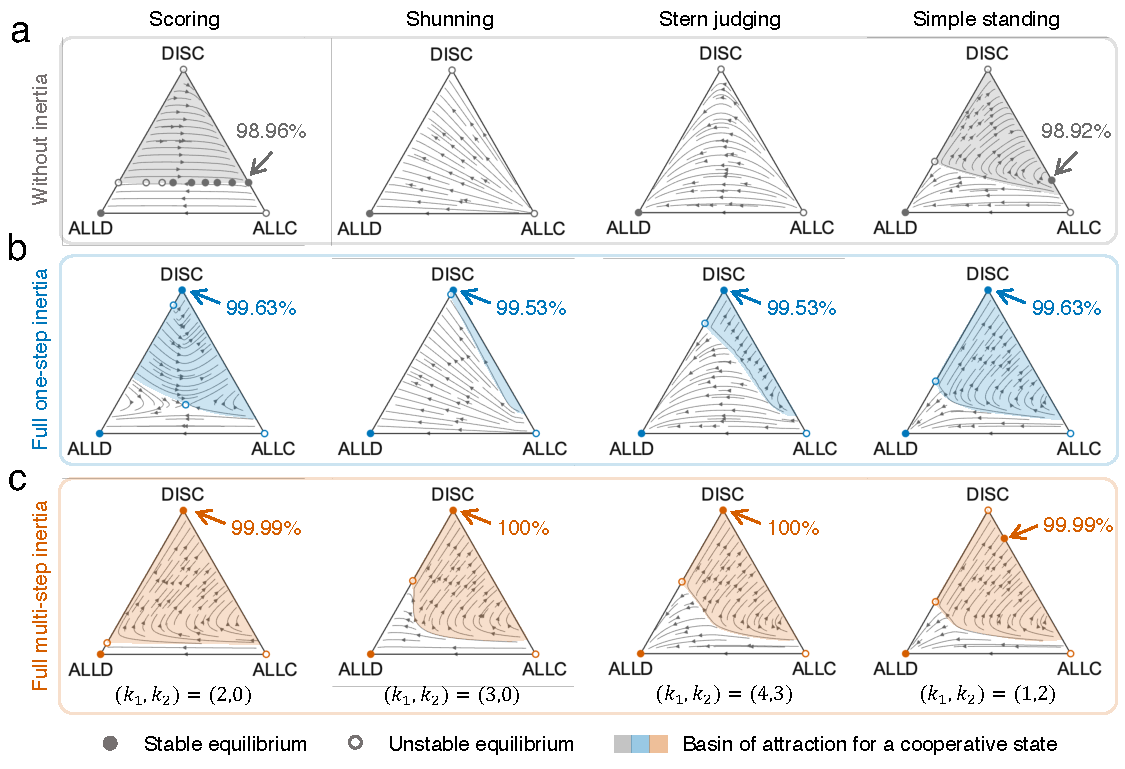
\includegraphics[width=\linewidth]{Fig3}
\caption{\textbf{Directional inertia reshapes the evolutionary dynamics of cooperation.}
\textbf{a--c}, Evolutionary dynamics of ALLC, ALLD and DISC under SC, SH, SJ and SS (columns) without inertia (\textbf{a}), with full one-step inertia (\textbf{b}) and with the selected multi-step architectures (\textbf{c}). Arrows indicate the direction of evolution. Filled and open circles denote stable and unstable equilibria, respectively. For equilibria on an edge of the simplex, markers refer to stability along that edge (Methods). Percentages give intended cooperation at the indicated equilibria, and shading marks the basin of attraction of a cooperative state. Without inertia, SC has a line of neutral equilibria on which all three payoffs are equal (Supplementary Note~\ref{si:evolution}). The selected depths $(k_1,k_2)$ are $(2,0)$, $(3,0)$, $(4,3)$ and $(1,2)$ for SC, SH, SJ and SS, respectively. Reputations are relaxed from initially good records at every composition. Parameters: $b/c=5$, $e_1=e_2=0.02$ and $\alpha=\beta=1$.
\draftnote{Draft: the SC panel in a has not yet been updated and will be replaced.}}
\label{fig:dynamics}
\end{figure}
% NOTE (3 Nov 2026): the Scoring panel of Fig. 3a is not final. The text above
% describes Fig. 3a only qualitatively; check the wording against the updated panel.

Whether an established discriminator population resists rare unconditional mutants has a compact analytical answer. Let $\rR$ denote the stationary probability that a resident DISC individual is regarded as good by an observer. When both denominators below are positive, pure DISC resists invasion by rare ALLD and ALLC mutants if and only if $b/c$ lies in the window
\begin{equation}
R_{\mathrm L}\equiv
\frac{\rR}{\rR-\Rmap\bigl[\rR\Pp{D|G}+(1-\rR)\Pp{D|B}\bigr]}
<\frac{b}{c}<
\frac{1-\rR}{\Rmap\bigl[\rR\Pp{C|G}+(1-\rR)\Pp{C|B}\bigr]-\rR}
\equiv R_{\mathrm U}.
\label{eq:window}
\end{equation}
Here $\Pp{D|G}$ and $\Pp{D|B}$ are the probabilities that an observer assesses a defecting donor, such as a rare ALLD mutant, positively when the observer regards the recipient as good or bad, respectively. $\Pp{C|G}$ and $\Pp{C|B}$ are the corresponding probabilities for a donor who intends to cooperate, such as a rare ALLC mutant. These probabilities are set by the norm and include both kinds of error (Methods). Because mutants are rare, their recipients are almost always residents, whom an observer regards as good with probability $\rR$. Each bracketed term is therefore the overall probability $u$ that the mutant's action is assessed positively. The reputation map $\Rmap(u)$ gives the stationary probability that an inertial record is read as good when each assessment is positive with probability $u$, and it depends on $k_1$, $k_2$, $\alpha$ and $\beta$ (Methods). The two bracketed reputations are thus the stationary reputations of rare ALLD and ALLC mutants, $r^*_{\ALLD}$ and $r^*_{\ALLC}$.

The window follows from a rare-mutant payoff comparison. Per round, and up to the common factor $1-e_1$, a resident earns $(b-c)\rR$, a rare ALLD mutant earns $b\,r^*_{\ALLD}$ and a rare ALLC mutant earns $b\,r^*_{\ALLC}-c$. Requiring the resident to earn more than each mutant gives the lower and upper bounds. The lower bound ensures that ALLD loses enough help to offset the cooperation cost it saves. The upper bound arises because ALLC also helps recipients that discriminators regard as bad and can gain a reputational advantage by doing so. We call pure DISC locally protected when $b/c$ lies in this window. Without inertia, no benefit-to-cost ratio protects pure DISC (Supplementary Note~\ref{si:unconditional}). Full one-step inertia opens the window, with $R_{\mathrm U}$ between $5.6$ and $6.3$, and the selected architectures extend it to $R_{\mathrm U}>200$ under SC, SH and SJ (Supplementary Table~\ref{tab:si-thresholds}). Under SS, the selected architecture has $R_{\mathrm U}\approx4.0$, below the reference value $b/c=5$. Pure DISC can therefore be invaded by ALLC under SS, and the population settles in the highly cooperative ALLC--DISC mixture instead of losing cooperation.

These outcomes are robust across the further conditions we examined, each of which tests a different property of the cooperative states. Starting from all-bad instead of all-good reputations leaves the mean cooperation of the selected architectures nearly unchanged, with a small residual difference under SJ ($0.699$ versus $0.706$; Extended Data Fig.~\ref{ed:resident}e--h). Under one-step inertia, by contrast, cooperation under SH and SJ collapses after all-bad initialization. The selected architectures support higher mean cooperation across most benefit-to-cost ratios, and under SS high cooperation persists even where pure DISC is not locally protected (Extended Data Fig.~\ref{ed:benefit-cost}). At one-step depths, tolerance alone, $(\alpha,\beta)=(1,0)$, and strictness alone, $(\alpha,\beta)=(0,1)$, have different, norm-dependent effects on the strategy dynamics (Extended Data Fig.~\ref{ed:readout}). Across implementation and assessment errors, the selected architectures exclude ALLD over most of the error plane under SH and SJ, and under SC and SH they protect pure DISC against both mutants over most of it (Extended Data Fig.~\ref{ed:errors}). Selected multi-step inertia thus yields near-complete intended cooperation at stable equilibria and enlarges their basins of attraction. Directional inertia turns reliable private reputations into an evolutionary advantage for cooperation. The selected architectures, however, differ in both total depth and allocation. We next isolate the role of allocation by comparing architectures with the same number of intermediate states.

% -----------------------------------------------------------------------------
\subsection*{The direction of inertia matters at a fixed depth}

To distinguish the effect of allocation from that of total depth, we compared all pairs $(k_1,k_2)$ with the same total depth $K$ and computed the mean realized cooperation $\bar\rho$ for each pair (Fig.~\ref{fig:depth}). At a given $K$, alternative allocations can produce very different levels of cooperation. With eight intermediate states under SC, for example, $\bar\rho$ ranges from zero when all states are recovery states to $0.875$ when all are warning states. The largest sampled values occur for tolerance-only allocations under SC and SH. High-performing SJ allocations at larger depths combine both paths, whereas SS favors one or two warning states combined with a longer recovery path. The full plane of depths shows the same patterns and also shows that local protection of pure DISC and high population-level cooperation are distinct properties (Extended Data Fig.~\ref{ed:depth-plane}). The four architectures selected solely from $\Delta g$ and $\bar d$ achieve the highest sampled cooperation at their respective total depths. Under these conditions, the two reputation criteria therefore identify compact architectures that also perform well in the evolutionary analysis.

\begin{figure}[tbp]
\centering
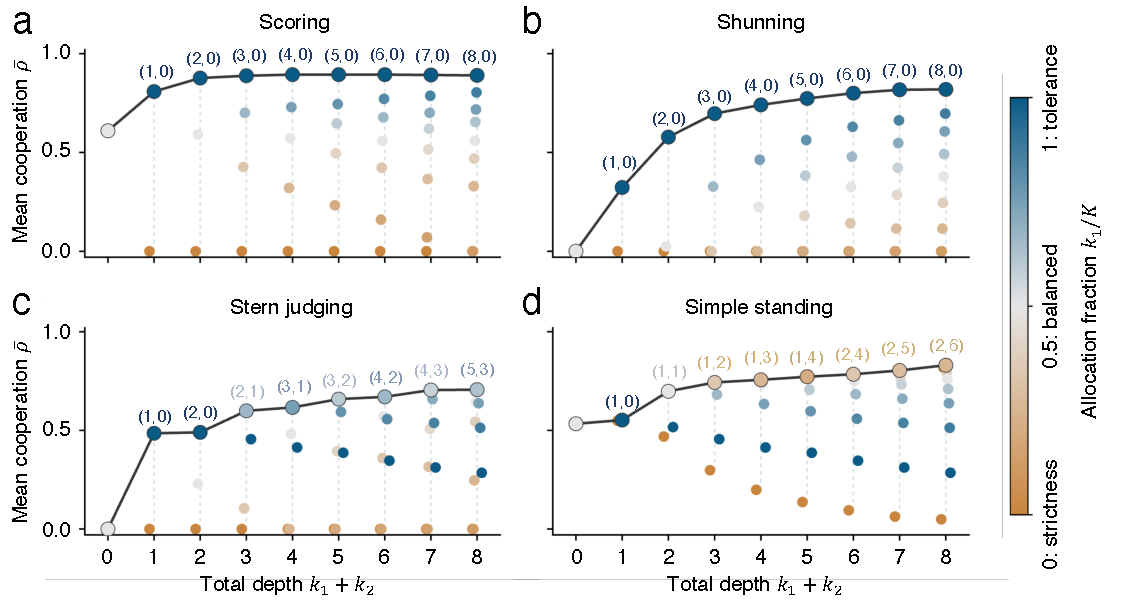
\includegraphics[width=\linewidth]{Fig4}
\caption{\textbf{More inertia does not always yield more cooperation.}
\textbf{a--d}, Mean realized cooperation $\bar\rho$ under SC (\textbf{a}), SH (\textbf{b}), SJ (\textbf{c}) and SS (\textbf{d}) as a function of total depth $K=k_1+k_2$. Each point represents one allocation $(k_1,k_2)$, with color indicating the tolerance fraction $k_1/K$. $K=0$ is the instantaneous baseline. Large outlined points connected by black lines identify the largest sampled mean at each $K$, with depth pairs labeled. Cooperation is averaged over 512 initial strategy compositions sampled uniformly from the simplex (Methods). Parameters: $b/c=5$, $e_1=e_2=0.02$ and $\alpha=\beta=1$.}
\label{fig:depth}
\end{figure}

Greater depth does not necessarily improve cooperation. Under SC, the highest sampled cooperation levels off from about $K=3$ ($0.879$) and does not increase further as $K$ grows ($0.888$ at $K=5$ and $0.875$ at $K=8$). Retaining more evidence therefore does not necessarily produce more cooperation. More generally, the benefit of additional depth depends on the norm and on how the depth is allocated, and an appropriately allocated intermediate depth already supports high cooperation. The evolutionary value of inertia thus depends on how a limited depth is divided between protecting and restoring standing. A moderate amount of appropriately allocated inertia can enhance cooperation, whereas adding states does not by itself guarantee further improvement. Because protecting good standing means tolerating some negative evidence, we next examine whether occasional defectors can exploit that tolerance.

% -----------------------------------------------------------------------------
\subsection*{Tolerance creates opportunistic risk, and tuning its strength moderates it}

Protecting a good reputation from isolated negative assessments helps DISC withstand imperfect information. Could an individual exploit that protection by occasionally withholding help? We introduce a rare opportunistic discriminator (O-DISC), which behaves like DISC except that, whenever it would help a recipient it regards as good, it withholds help with probability $\delta$, independently in each interaction. The endpoints $\delta=0$ and $\delta=1$ correspond to DISC and ALLD, respectively. Let $\rX(\delta)$ denote the stationary probability that the mutant is regarded as good. The mutant's payoff advantage over the resident, in units of the expected cost of an intended cooperative act, is
\begin{equation}
\Lambda(\delta)=\frac{\Pi_{\mathrm X}-\Pi_{\mathrm R}}{c(1-e_1)}
=\delta\rR-\frac{b}{c}\bigl[\rR-\rX(\delta)\bigr].
\label{eq:lambda}
\end{equation}
The first term is the cooperation cost the mutant saves, and the second is the benefit it loses through a worse reputation. A positive $\Lambda$ permits invasion. Showing that ALLD cannot invade tests only $\delta=1$ and does not address partial opportunism, $0<\delta<1$.

All five SJ mechanisms compared in Fig.~\ref{fig:opportunism}a exclude ALLD. Nevertheless, the selected multi-step architecture with full readout, full one-step inertia, aggregation of two sampled assessments\cite{michelmata2024} and a bounded quantitative score\cite{schmid2023} each admit a positive opportunistic window. Under the selected architecture $(4,3)$, every mutant with $0<\delta<0.365$ can invade, whereas the one-step window is narrow ($0<\delta<0.008$). The two alternative mechanisms serve as illustrations rather than benchmarks, because their parameters were neither optimized nor matched in memory to the inertial record (Supplementary Note~\ref{si:filters}). Tolerance can therefore make reputation systems vulnerable to opportunistic defection even when they exclude unconditional defectors.

\begin{figure}[tbp]
\centering
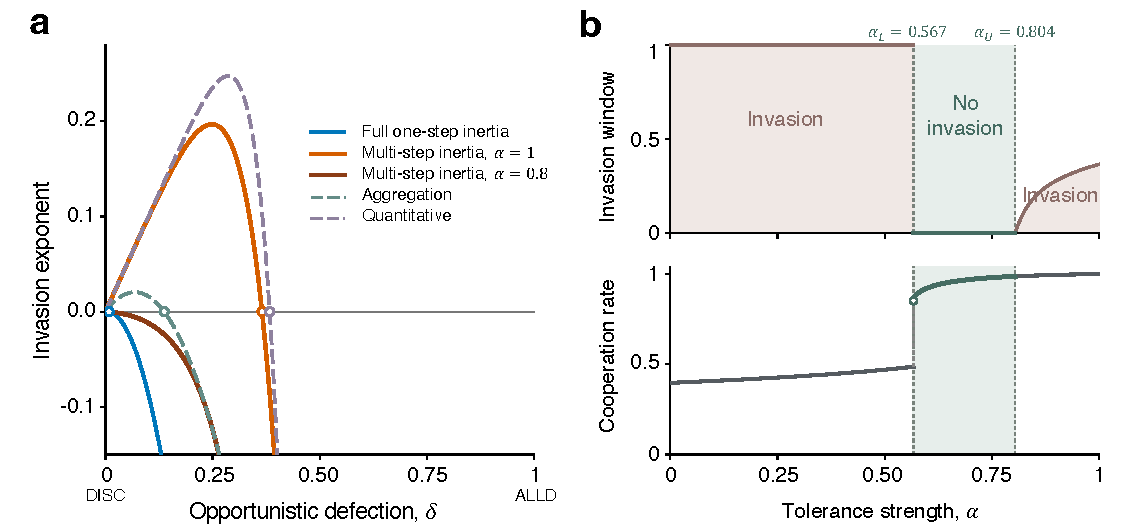
\includegraphics[width=\linewidth]{Fig5}
\caption{\textbf{Tolerance can permit opportunistic invasion, and reducing tolerance strength can limit it.}
\textbf{a}, Normalized payoff advantage $\Lambda$ of an O-DISC mutant against a DISC resident under SJ, as a function of the omission probability $\delta$ ($\delta=0$, DISC; $\delta=1$, ALLD). Curves compare full one-step inertia, the selected multi-step architecture $(4,3)$ with $\alpha=1$ and $\alpha=0.8$, an aggregation rule based on Michel-Mata et al.\cite{michelmata2024} and a quantitative score based on Schmid et al.\cite{schmid2023} Positive values indicate invasion, and open circles mark nonzero crossings.
\textbf{b}, Selected multi-step architecture $(4,3)$ as the tolerance strength $\alpha$ varies. The upper panel shows the largest detected endpoint $\delta_c$ of the invasion window, and the lower panel shows resident intended cooperation $\rR$. The green band marks the secure range $\alpha_{\mathrm L}<\alpha\leq\alpha_{\mathrm U}$, with $\alpha_{\mathrm L}=0.567$ and $\alpha_{\mathrm U}=0.804$. Parameters: $b/c=5$, $e_1=e_2=0.02$ and $\beta=1$.}
\label{fig:opportunism}
\end{figure}

The response to weak opportunism explains this window. The marginal invasion advantage at $\delta=0$ is
\begin{equation}
\Lambda'(0)=\rR\Bigl[1-\frac{b}{c}\,\dPhi\,\Rmap'(\uR)\Bigr].
\label{eq:lambda-slope}
\end{equation}
Here $\dPhi$ is the assessment contrast, the difference between the probabilities that intended cooperation and intended defection are assessed positively in the resident environment. $\Rmap'$ is the derivative of the reputation map with respect to the positive-assessment probability $u$, evaluated at the probability $\uR$ that a resident is assessed positively. The expression follows from $\rX(\delta)=\Rmap[\uX(\delta)]$, where $\uX(\delta)$ is the mutant's positive-assessment probability, because each unit of $\delta$ lowers $\uX$ by $\rR\dPhi$ (Methods). If the reputation response is too flat, a small omission barely lowers the mutant's reputation, and the saved cost dominates. Full tolerance readout produces such a flat response. For any architecture with a warning path ($k_1\geq1$), $\Rmap'(u)\to1-\alpha$ as $u\to1$ (Supplementary Note~\ref{si:map}), so the marginal penalty nearly vanishes near an all-good resident when $\alpha=1$. Reducing $\alpha$ gives warning states an immediate chance of being read as bad and can thereby increase the reputational cost of omission. The local slope alone, however, does not establish resistance for every $\delta$.

To assess all degrees of opportunism, we computed the reputation lost per unit of withheld cooperation, $H(\delta)=[\rR-\rX(\delta)]/(\delta\rR)$, and its smallest value over the mutant family. Because $\Lambda(\delta)\leq0$ exactly when $H(\delta)\geq c/b$, the resident excludes the entire family if and only if
\begin{equation}
\Hmin\equiv\min_{0\leq\delta\leq1}\frac{\rR-\rX(\delta)}{\delta\,\rR}\geq\frac{c}{b}.
\label{eq:security}
\end{equation}
At $\delta=0$ the ratio is defined by its limit, $\dPhi\,\Rmap'(\uR)$. The condition requires that even the mutant with the smallest reputational penalty gains no payoff advantage. Lowering $\alpha$ allows warning states to affect current treatment before the established reputation changes and can therefore strengthen the penalty for occasional defection.

Under SJ, the selected architecture with full tolerance strength ($\alpha=1$) admits an opportunistic window although ALLD is excluded. At $\alpha=0.8$, no O-DISC mutant can invade, and resident intended cooperation remains high ($\rR=0.987$). For this architecture, the marginal penalty $\dPhi\,\Rmap'(\uR)$ rises from $4.8\times10^{-5}$ at $\alpha=1$ to $0.204$ at $\alpha=0.8$, just above $c/b=0.2$ (Supplementary Note~\ref{si:opportunism}). Lowering the tolerance strength too far, however, eliminates the high-reputation resident state. The resulting secure range, in which the resident resists the entire O-DISC family while its high-reputation state persists, is $0.567<\alpha\leq0.804$ (Fig.~\ref{fig:opportunism}b). The lower boundary $\alpha_{\mathrm L}$ is a fold of the high-reputation resident state and does not depend on $b/c$. The upper boundary $\alpha_{\mathrm U}$ is the readout at which the weakest opportunists become neutral, and it rises with $b/c$ (Methods).

Protective readouts exist under all four norms, although their locations depend on the norm and the architecture (Extended Data Fig.~\ref{ed:security}). At $\alpha=0.8$ and $b/c=5$, all four selected architectures resist the tested O-DISC family, with resident intended cooperation between $0.978$ and $0.990$ (Supplementary Table~\ref{tab:si-secure}). Under one-step inertia, the outcome at this reference point depends on the norm, and SH and SJ have already lost their high-reputation resident state. Because resident reputations do not depend on $b/c$, the fold boundaries are fixed, whereas the upper boundaries rise with $b/c$. The secure interval can therefore close at low benefit-to-cost ratios, as under SH at $b/c=2$. These results concern the specified family of independent omissions. They do not establish resistance to persistent or temporally correlated opportunism, nor to ALLC. Under SS, the selected architecture resists O-DISC but can be invaded by ALLC.

Directional reputation inertia thus links private evidence accumulation to the emergence of cooperation. Allocating depth to the loss and recovery of standing can produce distinguishable, consistent reputations and highly cooperative evolutionary outcomes, while enlarging the basins of attraction of cooperative states. The tolerance strength of warning states determines whether incomplete negative evidence already affects treatment and, in the cases studied, can protect resident cooperation against occasional opportunistic defection.

% =============================================================================
\section*{Discussion}
\draftnote{Provisional Discussion, to be revised. It summarizes the findings, positions them and states limitations without adding new results.}

We have shown that the way a reputation system integrates behavioral evidence over time shapes both the quality of private reputations and the evolution of cooperation. Two separations underlie the framework. Losing and regaining standing follow different paths, and the accumulation of evidence is distinct from its readout. The depths $k_1$ and $k_2$ determine how much consistent evidence reverses an established reputation, whereas the strengths $\alpha$ and $\beta$ determine how strongly incomplete evidence already affects treatment. The direction in which depth is allocated, rather than its total amount, determined whether private observers agreed on discriminating judgments. The same allocations, selected without reference to evolutionary outcomes, supported highly cooperative outcomes with enlarged basins of attraction.

Previous mechanisms improve reputation-based cooperation under private information either by restoring agreement among observers\cite{radzvilavicius2021,kawakatsu2024,radzvilavicius2019,murase2024synchronization} or by changing how evidence is assessed and integrated.\cite{schmid2021,tanabe2013,schmid2023,michelmata2024} Inertial updating belongs to the second group but treats losing and regaining standing as separate processes. The allocations we identified differ systematically across norms. Inertia protects good standing under SC and SH, extends in both directions under SJ and lengthens recovery under SS. This pattern was obtained for four second-order norms and should not be read as a general rule.

Tolerance carries a cost. A reputation system that forgives isolated negative assessments also forgives deliberate occasional defection, so excluding unconditional defectors does not exclude partial opportunism. The same vulnerability appeared for aggregation and quantitative scoring in the settings we tested. Within the inertial framework, readout provides a remedy that leaves evidence accumulation unchanged. When warning states carry a partial social consequence, occasional defection becomes costly before an established reputation is lost. The principle can be summarized as accumulating evidence before changing a reputation while responding to that evidence along the way.

Our analysis has limitations (Supplementary Note~\ref{si:scope}). The population-level theory relies on a mean-field closure for private assessment, and strategy evolution is evaluated at stationary reputations. All individuals share the same inertial architecture, which does not itself evolve and carries no explicit memory cost. Resistance was tested against unconditional strategies and a family of independent omissions, not against temporally correlated or persistent exploitation. Future work could allow depths and readout strengths to evolve, consider structured populations and test empirically whether people update reputations with direction-dependent inertia.

% =============================================================================
\section*{Methods}
\label{sec:methods}
% Source: Methods.pdf. Equations displayed in the Results (Eqs. 1-4) are cited
% rather than repeated, and the conceptual description of Fig. 1 is given only
% in the Results. Extended Data numbers follow the figure files in Manuscript_doc.

\subsection*{Donation game, strategies and private assessment}

We consider an infinitely large, well-mixed population in which randomly chosen donors and recipients play the donation game. A donor either cooperates, paying a cost $c>0$ to give the recipient a benefit $b>c$, or defects, which has no payoff consequences. Individuals use one of three strategies $I\in\{\ALLC,\ALLD,\DISC\}$ with frequencies $f_I$, $\sum_If_I=1$. ALLC intends to cooperate with every recipient, ALLD intends to defect against every recipient, and DISC intends to cooperate if and only if it regards the recipient as good. All individuals share one social norm and one reputation mechanism, specified by the depths $k_1,k_2$ and the readout parameters $\alpha,\beta$. Strategy evolution changes only the frequencies $f_I$.

Reputations are private.\cite{okada2018,hilbe2018,radzvilavicius2019} Every individual keeps its own record of every other individual. In each interaction, an observer drawn independently of donor and recipient assesses the donor. A DISC donor chooses its action using its own image of the recipient, whereas the observer judges the donor's realized action using the observer's own image of the recipient, so the two can disagree. We use second-order norms.\cite{ohtsuki2004} Cooperation with a recipient regarded as good is assessed positively and defection against such a recipient negatively. Towards a recipient regarded as bad, cooperation and defection are assessed positively with probabilities $p$ and $q$, respectively. SC, SH, SJ and SS correspond to $(p,q)=(1,0)$, $(0,0)$, $(0,1)$ and $(1,1)$.

Intended cooperation fails and becomes defection with probability $e_1$, whereas intended defection is always implemented. After applying the norm, the observer records the opposite assessment with probability $e_2$. The two errors are independent, and benefits and costs accrue only for realized cooperation. Let $\Pp{A|Y}$ denote the probability that the recorded assessment is positive, given the donor's intended action $A\in\{\st C,\st D\}$ and the observer's image $Y\in\{\st G,\st B\}$ of the recipient. With $\varepsilon=(1-e_1)(1-e_2)+e_1e_2$,
\begin{equation}
\begin{aligned}
\Pp{C|G}&=\varepsilon, &\qquad \Pp{C|B}&=e_2+(1-2e_2)\bigl[(1-e_1)p+e_1q\bigr],\\
\Pp{D|G}&=e_2, &\qquad \Pp{D|B}&=e_2+(1-2e_2)q
\end{aligned}
\label{eq:m-assessment}
\end{equation}
(Supplementary Note~\ref{si:interactions}). Implementation error is already averaged into Eq.~\eqref{eq:m-assessment}. If the observer regards the recipient as good with probability $r$, intended cooperation and intended defection are therefore assessed positively with probabilities
\begin{equation}
\PhiC(r)=r\Pp{C|G}+(1-r)\Pp{C|B},\qquad
\PhiD(r)=r\Pp{D|G}+(1-r)\Pp{D|B},
\label{eq:m-phi}
\end{equation}
and their difference, the assessment contrast, is $\Delta\Phi(r)=\PhiC(r)-\PhiD(r)=\kappa[r+(p-q)(1-r)]$ with $\kappa=(1-e_1)(1-2e_2)$. Unless stated otherwise, $b=5$, $c=1$ and $e_1=e_2=0.02$.

\subsection*{Inertial reputation records and binary readout}

Observer $i$ holds a latent record $L_{ij}$ of target $j$ in the state space
\begin{equation}
\Lspace=\{\st G,\st W_1,\ldots,\st W_{k_1},\st B,\st S_1,\ldots,\st S_{k_2}\},\qquad k_1,k_2\in\{0,1,2,\ldots\}.
\label{eq:m-states}
\end{equation}
After each interaction, only the observer's record of the donor changes, and only through the recorded assessment. The transitions follow Fig.~\ref{fig:model}b. A negative assessment moves $\st G\to\st W_1\to\cdots\to\st W_{k_1}\to\st B$ and leaves $\st B$ unchanged. A positive assessment moves $\st B\to\st S_1\to\cdots\to\st S_{k_2}\to\st G$ and leaves $\st G$ unchanged. A positive assessment returns every warning state $\st W_m$ directly to $\st G$, and a negative assessment returns every recovery state $\st S_n$ directly to $\st B$ (direct reset). If $k_1=0$, a negative assessment moves $\st G$ directly to $\st B$, and if $k_2=0$, a positive assessment moves $\st B$ directly to $\st G$. Consecutive assessments are those made by the same observer about the same target. A record has $K+2$ states (complete transition table in Supplementary Note~\ref{si:record} and Supplementary Table~\ref{tab:si-transitions}).

Actions and assessments use a binary image that is sampled from the record whenever the record is consulted. The image is good with probability
\begin{equation}
\sigma(\st G)=1,\qquad \sigma(\st W_m)=\alpha^m,\qquad \sigma(\st B)=0,\qquad \sigma(\st S_n)=1-\beta^n,\qquad 0\leq\alpha,\beta\leq1.
\label{eq:m-readout}
\end{equation}
Consultations are independent given the current state and do not change it. Setting $\alpha=\beta=0$ at any depths also yields instantaneous updating, because the image then always equals the last recorded assessment (Supplementary Note~\ref{si:record}). At one-step depths, $(\alpha,\beta)=(1,0)$ and $(0,1)$ give tolerance-only and strictness-only readout. The selected multi-step architectures are obtained from simulated reputation statistics, as described below.

\subsection*{Stationary reputation map}

Consider one record whose successive recorded assessments are independent and positive with probability $u$. Its state then follows a Markov chain with transition matrix $T(u)=uT^++(1-u)T^-$, where $T^+$ and $T^-$ encode the deterministic updates after positive and negative assessments. For $0<u<1$ the chain is irreducible and aperiodic. Write $v=1-u$. Because $\st W_m$ can be entered only from $\st W_{m-1}$ (with $\st W_0\equiv\st G$) after a negative assessment, and $\st S_n$ only from $\st S_{n-1}$ (with $\st S_0\equiv\st B$) after a positive one, the stationary distribution satisfies $\pi_{\st W_m}=v^m\pi_{\st G}$ and $\pi_{\st S_n}=u^n\pi_{\st B}$. The only transitions from the good-standing states $\{\st G,\st W_m\}$ to the bad-standing states $\{\st B,\st S_n\}$ complete a run of $k_1+1$ negative assessments, and the only reverse transitions complete a run of $k_2+1$ positive assessments. Balancing these two fluxes gives $v^{k_1+1}\pi_{\st G}=u^{k_2+1}\pi_{\st B}$, and normalization yields
\begin{equation}
\pi_{\st G}=\frac{u^{k_2+1}}{Z(u)},\quad
\pi_{\st W_m}=\frac{v^mu^{k_2+1}}{Z(u)},\quad
\pi_{\st B}=\frac{v^{k_1+1}}{Z(u)},\quad
\pi_{\st S_n}=\frac{u^nv^{k_1+1}}{Z(u)},\quad
Z(u)=v^{k_1}+u^{k_2}-v^{k_1}u^{k_2}
\label{eq:m-stationary}
\end{equation}
(Supplementary Note~\ref{si:map}). Averaging the readout probabilities over this distribution defines the reputation map, the stationary probability that the target is regarded as good when it is assessed positively with probability $u$,
\begin{equation}
\Rmap(u)\equiv\Rmap(u;\alpha,\beta,k_1,k_2)=\sum_{\ell\in\Lspace}\pi_\ell(u)\,\sigma(\ell)
=\frac{u^{k_2+1}\sum_{m=0}^{k_1}(\alpha v)^m+v^{k_1+1}\sum_{n=1}^{k_2}u^n\bigl(1-\beta^n\bigr)}{v^{k_1}+u^{k_2}-v^{k_1}u^{k_2}}.
\label{eq:m-map}
\end{equation}
Empty sums are zero, and $\Rmap(0)=0$ and $\Rmap(1)=1$ by continuity. Without inertia, $\Rmap(u)=u$. For one-step inertia, $\Rmap(u)=\{u^2[1+\alpha(1-u)]+(1-\beta)u(1-u)^2\}/(1-u+u^2)$, and with full readout, $\Rmap(u)=u^{k_2}(1-v^{k_1+1})/Z(u)$. The map increases with $\alpha$ and decreases with $\beta$. Two further properties are used below. For $k_1\geq1$, $\Rmap'(1)=1-\alpha$, where the prime denotes $\dd/\dd u$, and for $k_2=0$, $\Rmap$ is concave on $[0,1]$ (Supplementary Note~\ref{si:map}).

\subsection*{Self-consistent private reputations}

Let $r_I$ be the probability that a randomly chosen observer regards a randomly chosen type-$I$ individual as good, and $\bar r=\sum_If_Ir_I$. We close the private-assessment problem with two mean-field assumptions, as in previous analyses of private assessment.\cite{okada2018,radzvilavicius2019,kessinger2023,michelmata2024,kawakatsu2024} First, the donor's and the observer's images of a recipient are independent given the recipient's strategy. Both then regard a random recipient as good with probability $h_{\mathrm{GG}}=\sum_Jf_Jr_J^2$, both regard it as bad with probability $h_{\mathrm{BB}}=\sum_Jf_J(1-r_J)^2$, and each of the two ordered disagreements occurs with probability $h_{\mathrm{GB}}=\sum_Jf_Jr_J(1-r_J)$. A type-$I$ donor is therefore assessed positively with probability
\begin{equation}
\begin{aligned}
u_{\ALLC}&=\PhiC(\bar r),\qquad u_{\ALLD}=\PhiD(\bar r),\\
u_{\DISC}&=h_{\mathrm{GG}}\Pp{C|G}+h_{\mathrm{GB}}\bigl(\Pp{C|B}+\Pp{D|G}\bigr)+h_{\mathrm{BB}}\Pp{D|B}.
\end{aligned}
\label{eq:m-u}
\end{equation}
Second, the assessments entering a record of a type-$I$ individual are treated as independent with this common probability $u_I$, so that each record has the stationary response of Eq.~\eqref{eq:m-map}. Stationary reputations then satisfy the self-consistency equations
\begin{equation}
r_I^*=\Rmap\bigl(u_I(\bm r^*;\bm f)\bigr),\qquad I\in\{\ALLC,\ALLD,\DISC\}.
\label{eq:m-selfconsistency}
\end{equation}
Equation~\eqref{eq:m-selfconsistency} can have several solutions. Consistent with records that start in good standing, we select at every composition the solution reached by the auxiliary relaxation
\begin{equation}
\frac{\dd r_I}{\dd\tau}=\Rmap(u_I)-r_I,\qquad r_I(0)=1.
\label{eq:m-relaxation}
\end{equation}
The variable $\tau$ is a computational time, unrelated to evolutionary time $t$. The fixed points of Eq.~\eqref{eq:m-relaxation} coincide with the stationary states of the mean-field dynamics of the full distribution of latent states, $\dd\bm\pi_I/\dd t'=\bm\pi_I[T(u_I)-\mathbf I]$ with $r_I=\bm\pi_I\bm\sigma$ (Supplementary Note~\ref{si:population}). Stability statements refer to Eq.~\eqref{eq:m-relaxation}. Where checked, they agreed with the linearization of the full latent-state system.

In a homogeneous DISC population with reputation $r$, a resident donor regards its recipient as good with probability $r$, independently of the observer, and Eq.~\eqref{eq:m-u} reduces to
\begin{equation}
u_{\mathrm R}(r)=r\,\PhiC(r)+(1-r)\,\PhiD(r).
\label{eq:m-resident}
\end{equation}
Resident reputations are the roots of $F(r)\equiv\Rmap[u_{\mathrm R}(r)]-r$, and their stability in Eq.~\eqref{eq:m-relaxation} is given by the sign of $F'(r)$. A fold of a resident branch satisfies $F(r)=F'(r)=0$, that is, $\Rmap'[u_{\mathrm R}(r)]\,u_{\mathrm R}'(r)=1$. We denote by $\rR$ the highest strictly stable root, which coincides with the root reached by relaxation from $r=1$ unless the highest root is a fold. We write $\uR=u_{\mathrm R}(\rR)$, $\Phi_A^*=\Phi_A(\rR)$ and $\dPhi=\Delta\Phi(\rR)$. Resident reputations do not depend on $b/c$.

\subsection*{Strategy evolution and cooperation}

Reputations are assumed to equilibrate quickly relative to strategy change. At each strategy composition, payoffs are evaluated with the selected stationary reputations. Per unit time, in which each individual acts on average once as donor and once as recipient, the expected payoffs are
\begin{equation}
\begin{aligned}
\Pi_{\ALLC}&=(1-e_1)\bigl[b\,(f_{\ALLC}+f_{\DISC}\,r^*_{\ALLC})-c\bigr],\\
\Pi_{\ALLD}&=(1-e_1)\,b\,(f_{\ALLC}+f_{\DISC}\,r^*_{\ALLD}),\\
\Pi_{\DISC}&=(1-e_1)\bigl[b\,(f_{\ALLC}+f_{\DISC}\,r^*_{\DISC})-c\,\bar r^*\bigr],
\end{aligned}
\label{eq:m-payoffs}
\end{equation}
and strategy frequencies follow the replicator dynamics\cite{hofbauer1998}
\begin{equation}
\frac{\dd f_I}{\dd t}=f_I\bigl(\Pi_I-\bar\Pi\bigr),\qquad \bar\Pi=\sum_Jf_J\Pi_J.
\label{eq:m-replicator}
\end{equation}
The intended and realized cooperation rates are $\rho_{\mathrm{int}}=f_{\ALLC}+f_{\DISC}\,\bar r^*$ and $\rho=(1-e_1)\rho_{\mathrm{int}}$, and $\bar\Pi=(b-c)\rho$. In a homogeneous DISC population, $\rho_{\mathrm{int}}=\rR$, and realized cooperation cannot exceed $1-e_1=0.98$.

To compare parameter settings globally, we integrate Eq.~\eqref{eq:m-replicator} from $n_{\mathrm{init}}=512$ initial compositions sampled uniformly by area from the simplex, using the same compositions for all settings that are compared. In every scan, each trajectory ended either in the zero-cooperation set or at an attractor with positive cooperation. The zero-cooperation set comprises the ALLD vertex together with the low-reputation segment of the ALLD--DISC edge, along which the dynamics drift slowly towards ALLD (final $\rho\leq7\times10^{-4}$). Attractors with positive cooperation have final $\rho\geq0.34$, and $0.974$--$0.980$ in nearly all conditions. We therefore define the cooperative basin as the set of initial compositions whose trajectories reach an attractor with positive cooperation, and classify a trajectory as cooperative if its final $\rho\geq0.01$. Any threshold inside the observed gap gives the same classification, and the gap was checked for every condition. We report the mean long-run cooperation $\bar\rho$ (the average of the final $\rho$ over initial compositions), the cooperative-basin size $\omega_{\mathrm C}$ (the fraction of cooperative trajectories) and the cooperation level $\bar\rho_{\mathrm C}$ within the basin, with $\bar\rho\approx\omega_{\mathrm C}\bar\rho_{\mathrm C}$. For the total-depth comparison (Fig.~\ref{fig:depth}), the envelope at total depth $K$ is the largest $\bar\rho$ among the $K+1$ allocations with $k_1+k_2=K$.

\subsection*{Invasion of a discriminator population}

We consider a homogeneous DISC population at $\rR$ and a rare mutant X that uses the residents' norm and record mechanism. Because the mutant is rare, it interacts with residents only and leaves their reputations and assessments unchanged. Suppose that X intends to help a resident recipient with probability $\chi_{\mathrm X}$, independently of the observer's image of that recipient, and acts independently across interactions. It is then assessed positively with probability $\uX=\chi_{\mathrm X}\Phi^*_{\mathrm C}+(1-\chi_{\mathrm X})\Phi^*_{\mathrm D}$, its stationary reputation is $\rX=\Rmap(\uX)$, and its normalized payoff advantage over residents is (Supplementary Note~\ref{si:unconditional})
\begin{equation}
\Lambda_{\mathrm X}\equiv\frac{\Pi_{\mathrm X}-\Pi_{\mathrm R}}{c(1-e_1)}
=\bigl(\rR-\chi_{\mathrm X}\bigr)-\frac{b}{c}\bigl(\rR-\rX\bigr),
\label{eq:m-mutant}
\end{equation}
the cooperation cost saved minus the benefit lost through reputation. The resident itself corresponds to $\chi=\rR$ and $u=\uR=\rR\Phi^*_{\mathrm C}+(1-\rR)\Phi^*_{\mathrm D}$.

\textit{Unconditional mutants.} ALLD ($\chi=0$) has reputation $\Rmap(\Phi^*_{\mathrm D})$ and ALLC ($\chi=1$) has reputation $\Rmap(\Phi^*_{\mathrm C})$, where $\Phi^*_{\mathrm D}=\rR\Pp{D|G}+(1-\rR)\Pp{D|B}$ and $\Phi^*_{\mathrm C}$ is defined analogously. When ALLD is regarded worse and ALLC better than the residents, Eq.~\eqref{eq:m-mutant} implies that the discriminator population resists both mutants if and only if $b/c$ lies in the window of Eq.~\eqref{eq:window}. If ALLD is not regarded worse than the residents, no $b/c$ excludes it. If ALLC is not regarded better, it cannot invade. Because $\uR=\rR\Phi^*_{\mathrm C}+(1-\rR)\Phi^*_{\mathrm D}$, the window is non-empty if and only if $\rR\Rmap(\Phi^*_{\mathrm C})+(1-\rR)\Rmap(\Phi^*_{\mathrm D})<\Rmap(\uR)$, that is, if $\Rmap$ at the resident's assessment probability lies above the chord joining its values at $\Phi^*_{\mathrm D}$ and $\Phi^*_{\mathrm C}$. Without inertia, $\Rmap$ is linear and $R_{\mathrm L}=R_{\mathrm U}=1/\dPhi$, so no benefit-to-cost ratio protects a discriminator population (Supplementary Note~\ref{si:unconditional}). Numerically, we classify local outcomes from the signs of the unnormalized payoff differences $\lambda_{\ALLD}=\Pi_{\ALLD}-\Pi_{\mathrm R}$ and $\lambda_{\ALLC}=\Pi_{\ALLC}-\Pi_{\mathrm R}$ (with $c=1$), which also covers cases without finite thresholds. ALLD is not excluded if $\lambda_{\ALLD}\geq-10^{-10}$. Otherwise, ALLC invades if $\lambda_{\ALLC}>10^{-10}$, and the residents resist both mutants if neither condition holds.

\textit{Opportunistic discriminators.} The opportunistic discriminator (O-DISC) defined in the Results replaces each intended cooperation, independently and before implementation error, by intended defection with probability $\delta\in[0,1]$. Thus $\chi=(1-\delta)\rR$. Its positive-assessment probability and reputation are
\begin{equation}
\uX(\delta)=\uR-\delta\,\rR\,\dPhi,\qquad \rX(\delta)=\Rmap\bigl[\uX(\delta)\bigr],
\label{eq:m-odisc}
\end{equation}
and Eq.~\eqref{eq:m-mutant} gives the normalized invasion payoff of Eq.~\eqref{eq:lambda} and its slope at the resident, Eq.~\eqref{eq:lambda-slope}. By construction, $\Lambda(0)=0$, and $\Lambda(1)$ is the normalized advantage of ALLD. For $\rR>0$, $\Lambda(\delta)=\delta\rR[1-(b/c)H(\delta)]$, where $H(\delta)=[\rR-\rX(\delta)]/(\delta\rR)$ is the reputation lost per unit of withheld cooperation, extended continuously by $H(0)=\dPhi\,\Rmap'(\uR)$. The residents therefore exclude every O-DISC mutant if and only if Eq.~\eqref{eq:security} holds, with equality permitting neutral mutants. Because $H(\delta)$ equals $\dPhi$ times the slope of the chord of $\Rmap$ between $\uX(\delta)$ and $\uR$, for $\dPhi>0$ the minimum is attained at $\delta\to0$ whenever $\Rmap$ is concave on that interval, which always holds for $k_2=0$. Equation~\eqref{eq:security} then reduces to $\Lambda'(0)\leq0$. In general, the whole interval must be checked. Near an all-good resident with $k_1\geq1$, $\Rmap'(\uR)\approx1-\alpha$, so full tolerance readout makes weak opportunism cheap. In the error-free limit with $\beta=1$ and $k_1\geq1$, an all-good resident excludes every O-DISC mutant if and only if $\alpha\leq1-c/b$, for every norm and every $k_2$ (Supplementary Note~\ref{si:opportunism}). At $b/c=5$ this bound is the readout $\alpha=0.8$ used in Fig.~\ref{fig:opportunism} and Extended Data Fig.~\ref{ed:security}.

For fixed norm, depths, $\beta$ and errors, a readout $\alpha$ is secure if a strictly stable high-reputation resident exists and satisfies Eq.~\eqref{eq:security}. The lower boundary $\alpha_{\mathrm L}$ of a secure interval, when it is not $\alpha=0$, is a fold of the high-reputation branch, $F(r,\alpha)=\partial_rF(r,\alpha)=0$ with $F(r,\alpha)=\Rmap[u_{\mathrm R}(r);\alpha,\beta,k_1,k_2]-r$. The fold itself is excluded and does not depend on $b/c$. The upper boundary $\alpha_{\mathrm U}$, when it is not $\alpha=1$, is where Eq.~\eqref{eq:security} holds with equality. In every case we computed, it was determined by $\delta\to0$, that is, by $(b/c)\,\Delta\Phi(r)\,\Rmap'[u_{\mathrm R}(r);\alpha_{\mathrm U}]=1$ together with $F(r,\alpha_{\mathrm U})=0$. When the fold and the local condition meet, the secure interval closes. This happens at $b/c=u_{\mathrm R}'(r)/\Delta\Phi(r)$ evaluated at the fold, which equals 2 for Shunning (Supplementary Note~\ref{si:opportunism}).

\textit{Alternative reputation filters.} For Fig.~\ref{fig:opportunism}a we replace $\Rmap$ by the stationary response of two alternative mechanisms while keeping the norm, errors, resident selection and Eqs.~\eqref{eq:lambda}, \eqref{eq:lambda-slope} and \eqref{eq:m-odisc} unchanged. Aggregation, adapted from Michel-Mata et al.,\cite{michelmata2024} assigns a good image if at least $Q$ of $M$ independently sampled assessments are positive, $\Rmap_{\mathrm{agg}}(u)=\sum_{j=Q}^{M}\binom{M}{j}u^j(1-u)^{M-j}$, with $(M,Q)=(2,1)$, so that $\Rmap_{\mathrm{agg}}(u)=2u-u^2$. Quantitative assessment, adapted from Schmid et al.,\cite{schmid2023} keeps an integer score $z\in\{-z_{\max},\ldots,z_{\max}\}$ that moves up or down by one after a positive or negative assessment and is read as good if $z\geq z_0$. Attempts to leave the range leave the score unchanged. With $t=u/(1-u)$, $\Rmap_{\mathrm{score}}(u)=\sum_{j=z_{\max}+z_0}^{2z_{\max}}t^j\big/\sum_{j=0}^{2z_{\max}}t^j$, and we use $z_{\max}=5$ and $z_0=0$. Neither mechanism was optimized or matched in memory to the inertial record.

\subsection*{Finite-population reputation simulations}

Individual-based simulations test reputation formation without the mean-field closure, at fixed strategy composition. They do not simulate strategy evolution. A population of $N$ individuals contains fixed numbers $n_I$ of each strategy. Every DISC individual stores a latent record of every individual, including itself, and all records start in $\st G$. Records held by ALLC and ALLD individuals are not stored because they never affect actions or assessments. Each event consists of five steps. (i) A donor is drawn uniformly from the population and a recipient uniformly from the remaining $N-1$ individuals, and an observer is drawn independently and uniformly from the DISC individuals. The observer may coincide with the donor or the recipient. (ii) The donor forms its intended action, a DISC donor by sampling its own image of the recipient from Eq.~\eqref{eq:m-readout}. (iii) Implementation error is applied. (iv) The observer independently samples its own image of the recipient, applies the norm to the realized action and reverses the assessment with probability $e_2$. (v) The observer's record of the donor is updated. A sweep consists of $n_{\DISC}N$ events, one update per stored record on average.

At sampled times we use $s_{ij}=\sigma(L_{ij})$, which averages exactly over readout randomness. For target $j$, the mean goodness and the probability that two distinct DISC observers give different images are
\begin{equation}
g_j=\frac{1}{n_{\DISC}}\sum_is_{ij},\qquad
d_j=\binom{n_{\DISC}}{2}^{-1}\sum_{i<i'}\bigl[s_{ij}(1-s_{i'j})+(1-s_{ij})s_{i'j}\bigr],
\label{eq:m-estimators}
\end{equation}
where $i$ and $i'$ run over DISC observers. Averaging over type-$I$ targets gives $g_I$ and $d_I$, which are then averaged over sampling times. The reputational separation and the mean disagreement used in Fig.~\ref{fig:recognition} and Extended Data Fig.~\ref{ed:selection} are
\begin{equation}
\Delta g=\frac{g_{\DISC}+g_{\ALLC}}{2}-g_{\ALLD},\qquad \bar d=\sum_I\frac{n_I}{N}\,d_I.
\label{eq:m-recognition}
\end{equation}
Unlike the mean-field theory, the simulations retain target-specific variation and correlations between the private records of different observers.

The recognition analyses use equal strategy numbers, $\alpha=\beta=1$ and $0\leq k_1,k_2\leq6$. Each run lasts 1,000 sweeps and is sampled every five sweeps from sweep 800 to sweep 1,000 (41 samples). The depth maps in Fig.~\ref{fig:recognition}e--h use one run per condition with $N=150$. The replicated analysis (Extended Data Fig.~\ref{ed:selection}) uses 30 independent runs per condition with $N=150$ and reports means across runs, with pointwise 95\% percentile intervals from 2,000 bootstrap resamples of the run means. A condition is eligible for selection if, for both $\Delta g$ and $\bar d$, the bootstrap interval of the difference between the second- and first-half means of the sampling window lies within $(-0.01,0.01)$. Two slowly relaxing SJ conditions required longer runs, $(k_1,k_2)=(4,5)$ with 3,000 sweeps (sampled from sweep 2,400) and $(3,5)$ with 50,000 sweeps (sampled from sweep 40,000). All 196 conditions then passed. Among eligible conditions with $\Delta g\geq0.8$ and $\bar d\leq0.1$, we select the smallest $K$, breaking ties by larger $\Delta g$, then smaller $\bar d$, $k_1$ and $k_2$. This gives the four selected architectures. The stars in Fig.~\ref{fig:recognition}e--h apply the same cutoffs and tie-breaking rule to the single-run maps, without the drift criterion, and identify the same four architectures. Selection uses reputation statistics only. The robustness analysis varies the separation cutoff from 0.70 to 0.90 in steps of 0.05 and the disagreement cutoff from 0.050 to 0.150 in steps of 0.025. The illustrative image matrices in Fig.~\ref{fig:recognition}a--d are final states of single runs with $N=90$ after 1,000 sweeps.

\subsection*{Numerical procedures and figure-specific settings}

All panels use $b/c=5$ and $e_1=e_2=0.02$ unless an axis varies them. Supplementary Note~\ref{si:settings} (Supplementary Table~\ref{tab:si-settings}) lists every setting, grid and tolerance. $\Rmap$ and $\Rmap'$ are evaluated in closed form. Homogeneous-DISC roots (Fig.~\ref{fig:opportunism} and Extended Data Figs.~\ref{ed:resident}a--d, \ref{ed:reputation-planes} and~\ref{ed:security}) are located by evaluating $F(r)$ on a fine uniform grid, refining sign changes by bracketing and classifying roots by the sign of $F'(r)$. At mixed compositions, Eq.~\eqref{eq:m-relaxation} is integrated from $r_I=1$ by fourth-order Runge--Kutta steps until $\max_I|\Rmap(u_I)-r_I|\leq10^{-11}$ ($10^{-12}$ for Fig.~\ref{fig:dynamics}). For local invasion (Extended Data Figs.~\ref{ed:benefit-cost}--\ref{ed:depth-plane}), the resident relaxation is followed by step-limited Newton refinement, which keeps the branch reached from $r=1$, to residual $\leq10^{-13}$.

All sampled-cooperation results (Fig.~\ref{fig:depth} and Extended Data Figs.~\ref{ed:resident}e--h, \ref{ed:benefit-cost}, \ref{ed:readout}e--h and~\ref{ed:depth-plane}) use one engine. Selected reputations are tabulated exactly on a triangular lattice with 120 subdivisions and interpolated linearly only inside cells in which no reputation component varies by more than 0.02. Elsewhere, including every cell crossed by a fold, they are computed exactly at the requested composition. Payoffs and the replicator field are always computed from these reputations, never interpolated. Trajectories are integrated with the explicit midpoint rule ($\Delta t=0.2$) until $\rho_{\mathrm{int}}$ changes by at most $10^{-7}$ over each of three consecutive intervals of 100 time units, or for at most $4\times10^4$ time units. Halving the step, refining the lattice and tightening the tolerances changed $\bar\rho$ by at most $1.3\times10^{-5}$ and changed no outcome class. Initial compositions are 512 points of a randomly shifted Halton sequence (bases 2 and 3, seed 2026) or, for Extended Data Fig.~\ref{ed:benefit-cost}, eight independently scrambled 512-point Sobol sequences\cite{virtanen2020} (seeds 2026--2033). Points are mapped area-uniformly onto the simplex by reflecting points of the unit square with $x+y>1$. In Extended Data Fig.~\ref{ed:benefit-cost}, standard errors are computed across the eight samples and therefore describe the sampling of initial compositions. The dynamics themselves are deterministic. Extended Data Fig.~\ref{ed:resident}e--h initializes reputations once, at $t=0$, as all-good or all-bad and then follows them quasi-statically along each trajectory by warm-started relaxation, so that a branch is left only where it ends.

In Fig.~\ref{fig:dynamics} and Extended Data Fig.~\ref{ed:readout}a--d, reputations are relaxed exactly at every point of an $84\times74$ grid clipped to the simplex. Vertex stability follows from the two rare-strategy growth rates. Edge equilibria are located on 501-point edge scans, and their markers refer to stability along the edge. Interior equilibria are classified by their Jacobian. Under SC without inertia, all three payoffs are equal on the line $f_{\DISC}=c/[b(\varepsilon-e_2)]\approx0.2126$ (Supplementary Note~\ref{si:evolution}). Extended Data Fig.~\ref{ed:reputation-planes} reports the highest stable homogeneous-DISC root and marks bistability (one-step readout plane, $161\times161$; depth plane, $0\leq k_1,k_2\leq8$). For every root in the depth planes, stability in Eq.~\eqref{eq:m-relaxation} agreed with the linearization of the full latent-state dynamics. On the ALLD--DISC edge (Extended Data Fig.~\ref{ed:edge}), Eq.~\eqref{eq:m-selfconsistency} reduces exactly to one equation in $\bar r$, which is solved for 1,071 values of $f_{\DISC}\in[0.01,1]$. Local invasion maps use $241\times241$ points of $e_1,e_2\in[0,0.45]$ (Extended Data Fig.~\ref{ed:errors}) and $801\times801$ points of $(\alpha,\beta)$ (Extended Data Fig.~\ref{ed:readout}i--l). In Fig.~\ref{fig:opportunism}, $\Lambda(\delta)$ is evaluated at 5,015 values of $\delta$, concentrated near $\delta=0$, with sign changes refined by Brent's method. The endpoint $\delta_c$ is the upper end of the interval with $\Lambda>0$. Residents of the alternative filters are obtained from $r=1$ by damped iteration, $r\leftarrow0.8r+0.2\,\Rmap_{\mathrm X}[u_{\mathrm R}(r)]$ with $\Rmap_{\mathrm X}\in\{\Rmap_{\mathrm{agg}},\Rmap_{\mathrm{score}}\}$. For Extended Data Fig.~\ref{ed:security} (at least 601 values of $\alpha$, 161 values of $b/c\in[2,8]$ and $\beta=1$), $\min_\delta H(\delta)$ is found by comparing $H$ at $\delta=0$, $\delta=1$ and all real roots in $(10^{-8},1)$ of the numerator of the rational function $\dd H/\dd\delta$. A readout is classified as secure if $1-(b/c)\min_\delta H\leq10^{-10}$. Fold endpoints are excluded, whereas endpoints at the domain boundary or at neutral invasion are included.

\subsection*{Data availability}
All numerical data underlying the figures are included in the verified computational package that accompanies the paper (Supplementary Note~\ref{si:settings}). \draftnote{Repository and DOI to be added before submission.}

\subsection*{Code availability}
The code and figure scripts used in this study are provided in the same package, with one notebook per figure, a C engine for the strategy dynamics, input configurations, validation records and checksums. \draftnote{Repository and DOI to be added before submission.}

% =============================================================================
\bibliography{references}

\section*{Acknowledgements}
\draftnote{To be added.}

\section*{Author contributions}
\draftnote{To be added.}

\section*{Competing interests}
\draftnote{To be added.}

% =============================================================================
% Extended Data figures (legends from Results_Outline.docx)
% =============================================================================
\clearpage
\setcounter{figure}{0}
\renewcommand{\figurename}{Extended Data Fig.}
\renewcommand{\theHfigure}{ED\arabic{figure}}

\section*{Extended Data}

\begin{figure}[!htbp]
\centering
\figfile{ED_Fig1}
\caption{\textbf{Selection and robustness of representative inertia architectures.}
\textbf{a--d}, Reputational separation $\Delta g$ and mean observer disagreement $\bar d$ for the tested depth pairs under SC, SH, SJ and SS, respectively. Points are colored by total depth $K=k_1+k_2$, and the shaded region marks the joint criteria $\Delta g\geq0.8$ and $\bar d\leq0.1$. Stars identify the qualifying pairs with the smallest $K$, namely $(2,0)$, $(3,0)$, $(4,3)$ and $(1,2)$, respectively. Insets display the wider parameter space, with open squares marking instantaneous updating.
\textbf{e--h}, Minimum-depth pair selected when the minimum separation and the maximum disagreement are varied. Orange boxes mark the default criteria, and dark outlines mark the region that retains the default selection. Although the exact depth pairs depend on the thresholds, compact qualifying architectures persist over a range of criteria. Each estimate averages 30 independent simulations, and only conditions that pass the drift criterion are eligible (Methods). Parameters: equal proportions of the three strategies, $N=150$, $e_1=e_2=0.02$ and $\alpha=\beta=1$.}
\label{ed:selection}
\end{figure}

\begin{figure}[!htbp]
\centering
\figfile{ED_Fig2}
\caption{\textbf{Reputation equilibria and population outcomes under contrasting initial reputations.}
\textbf{a--d}, Reputation dynamics in homogeneous DISC populations under SC, SH, SJ and SS, shown as the rate of change of the DISC good-reputation probability $r_{\DISC}$ in the auxiliary relaxation (Methods). Gray, blue and red curves represent instantaneous updating, full one-step inertia and the selected multi-step architectures, respectively. Filled and open circles denote stable and unstable equilibria, and arrows indicate the direction of the reputation dynamics. Full one-step inertia supports both high and low stable reputation states under SC, SH and SJ, whereas the selected multi-step architectures yield a single high-reputation equilibrium.
\textbf{e--h}, Mean realized cooperation $\bar\rho$ across initial strategy compositions under SC, SH, SJ and SS after all-good (solid bars) and all-bad (hatched bars) initial reputations. The selected multi-step architectures produce similar mean cooperation under both initial conditions, with a small residual difference under SJ. Under one-step inertia, cooperation under SH and SJ collapses after all-bad initialization. Parameters: $b/c=5$, $e_1=e_2=0.02$ and $\alpha=\beta=1$.}
\label{ed:resident}
\end{figure}

\begin{figure}[!htbp]
\centering
\figfile{ED_Fig3}
\caption{\textbf{Tolerance, strictness and depth jointly determine reputation equilibria.}
\textbf{a--d}, Highest stable good-reputation equilibrium in a homogeneous DISC population across tolerance strength $\alpha$ and strictness strength $\beta$ under one-step inertia ($k_1=k_2=1$), for SC, SH, SJ and SS.
\textbf{e--h}, Highest stable equilibrium across tolerance depth $k_1$ and strictness depth $k_2$ under full readout ($\alpha=\beta=1$). Color denotes the equilibrium good-reputation probability, and hatching identifies bistability in the homogeneous-DISC reputation dynamics. Open and blue squares mark instantaneous updating and full one-step inertia, and stars mark the selected multi-step architectures. High-reputation equilibria and the presence of bistability depend on the norm and on the direction and strength of inertia. Parameters: $e_1=e_2=0.02$.}
\label{ed:reputation-planes}
\end{figure}

\begin{figure}[!htbp]
\centering
\figfile{ED_Fig4}
\caption{\textbf{Reputation branches and payoff thresholds on the ALLD--DISC edge.}
\textbf{a--d}, Equilibrium good reputation of DISC, $r_{\DISC}$, as its frequency $f_{\DISC}$ varies along the ALLD--DISC edge under SC, SH, SJ and SS. Gray, blue and orange show instantaneous updating, full one-step inertia and selected multi-step inertia. Solid and dashed curves are stable and unstable reputation equilibria, respectively, and open diamonds mark folds where branches meet.
\textbf{e--h}, Corresponding normalized payoff advantage of DISC over ALLD on the branch selected by all-good initialization. Filled circles mark continuous edge equilibria, and triangles mark discontinuous changes in payoff sign at folds. Under one-step SC, SH and SJ, the high-reputation branch disappears when DISC becomes sufficiently rare, causing an abrupt loss of its payoff advantage. The selected multi-step architecture moves this threshold to lower DISC frequencies under SH and removes the fold under SC and SJ, where the threshold becomes a continuous edge equilibrium. Under SS, all thresholds are continuous. Parameters: $b/c=5$, $e_1=e_2=0.02$ and, for the inertial settings, $\alpha=\beta=1$.}
\label{ed:edge}
\end{figure}

\begin{figure}[!htbp]
\centering
\figfile{ED_Fig5}
\caption{\textbf{Cooperation and local discriminator protection across benefit-to-cost ratios.}
\textbf{a--d}, Mean cooperation $\bar\rho$ across initial strategy compositions as $b/c$ varies under SC, SH, SJ and SS. Gray, blue and orange lines denote instantaneous updating, full one-step inertia and the selected multi-step architectures. Solid segments indicate local protection of pure DISC against ALLC and ALLD ($R_{\mathrm L}<b/c<R_{\mathrm U}$; Eq.~\eqref{eq:window}), whereas dashed segments indicate that at least one of these mutants can invade pure DISC. Labels give the window bounds, and arrowheads indicate $R_{\mathrm U}>10$. The vertical dotted line marks $b/c=5$. Curves are means over eight independent samples of 512 initial compositions (Methods). Selected multi-step inertia supports higher mean cooperation across much of the range. Under SS, high cooperation can persist even where pure DISC is not locally protected. Parameters: $e_1=e_2=0.02$ and $\alpha=\beta=1$.}
\label{ed:benefit-cost}
\end{figure}

\begin{figure}[!htbp]
\centering
\figfile[0.6]{ED_Fig6}
\caption{\textbf{Separate effects of tolerance and strictness on strategy dynamics.}
\textbf{a--d}, Strategy dynamics under SC, SH, SJ and SS. In each column, the upper simplex shows tolerance only, $(\alpha,\beta)=(1,0)$, and the lower simplex shows strictness only, $(\alpha,\beta)=(0,1)$. Arrows indicate the direction of evolution, filled and open circles denote stable and unstable equilibria, shading marks the cooperative basin, and percentages indicate intended cooperation at the highlighted equilibria.
\textbf{e--h}, Mean cooperation $\bar\rho$ across the one-step $(\alpha,\beta)$ plane.
\textbf{i--l}, Local invasion classes for a pure-DISC resident. Pink indicates that ALLD invades, purple that ALLD is excluded but ALLC invades, and green that DISC resists both mutants. Tolerance and strictness have different, norm-dependent effects on strategy dynamics. Parameters: $b/c=5$, $e_1=e_2=0.02$ and $k_1=k_2=1$.}
\label{ed:readout}
\end{figure}

\begin{figure}[!htbp]
\centering
\figfile{ED_Fig7}
\caption{\textbf{Local invasion resistance across implementation and assessment errors.}
\textbf{a--c}, Local invasion classes of a pure-DISC resident across implementation error $e_1$ and assessment error $e_2$ under instantaneous updating (\textbf{a}), full one-step inertia (\textbf{b}) and selected multi-step inertia (\textbf{c}), with SC, SH, SJ and SS in columns. Pink denotes that ALLD invades, purple that ALLD is excluded but ALLC invades, and green that DISC resists both mutants. Without inertia or with one-step inertia, ALLD invades almost everywhere under SH and SJ. Selected multi-step inertia excludes ALLD over most of the error plane under these norms and, under SC and SH, makes DISC resistant to both mutants over most of it. These maps concern local resistance only and are not cooperation scans. Parameters: $b/c=5$ and $\alpha=\beta=1$.}
\label{ed:errors}
\end{figure}

\begin{figure}[!htbp]
\centering
\figfile{ED_Fig8}
\caption{\textbf{Mean cooperation and local discriminator protection across inertia depths.}
\textbf{a--d}, Mean realized cooperation $\bar\rho$ over the $(k_1,k_2)$ plane under SC, SH, SJ and SS, respectively. Color denotes cooperation averaged over initial strategy compositions, and dots identify depth pairs at which a pure-DISC population resists rare ALLC and ALLD mutants. SC and SH show high cooperation for tolerance-dominated allocations, SJ benefits from a combination of tolerance and strictness depths, and SS supports high cooperation whenever a warning path is present, with the highest values for strictness-weighted allocations. The dots also show that protection of pure DISC and high population-level cooperation are not identical. Parameters: $b/c=5$, $e_1=e_2=0.02$ and $\alpha=\beta=1$.}
\label{ed:depth-plane}
\end{figure}

\begin{figure}[!htbp]
\centering
\figfile{ED_Fig9}
\caption{\textbf{Tolerance strength and benefit-to-cost ratio shape resistance to opportunistic defection.}
\textbf{a}, Secure intervals in which an established DISC population resists the tested O-DISC family at $b/c=5$, comparing the one-step architecture $(k_1,k_2)=(1,1)$ with the selected multi-step architecture for each norm. Blue shading gives resident intended cooperation. Black outlines identify numerically secure intervals, and interval endpoints that coincide with branch folds are excluded.
\textbf{b--e}, Resident intended cooperation and O-DISC security across $\alpha$ and $b/c$ under SC, SH, SJ and SS, respectively. The upper and lower rows show one-step and selected multi-step inertia. Black curves delimit the secure region, and white circles mark $(\alpha,b/c)=(0.8,5)$. At this reference point the selected multi-step architectures maintain high resident cooperation and resist the tested opportunistic family under all four norms, whereas the outcome under one-step inertia depends on the norm. Security against O-DISC and high resident cooperation are distinct quantities. The selected multi-step depths are $(2,0)$, $(3,0)$, $(4,3)$ and $(1,2)$ for SC, SH, SJ and SS, respectively. Parameters: $e_1=e_2=0.02$ and $\beta=1$.}
\label{ed:security}
\end{figure}

% =============================================================================
% Supplementary Information
% Source: Supplementary_Information.pdf. Content preserved; Extended Data
% numbers updated to the figure files (ED6 readout, ED7 errors, ED8 depth plane,
% ED2e-h initial reputations); British spellings harmonized to American.
% =============================================================================
\clearpage
\renewcommand{\figurename}{Supplementary Fig.}
\renewcommand{\theHfigure}{SI\arabic{figure}}
\setcounter{figure}{0}
\setcounter{table}{0}
\setcounter{equation}{0}
\setcounter{section}{0}
\renewcommand{\thetable}{S\arabic{table}}
\renewcommand{\theHtable}{S\arabic{table}}
\renewcommand{\theequation}{S\arabic{equation}}
\renewcommand{\theHequation}{S\arabic{equation}}
\renewcommand{\thesection}{\arabic{section}}
\renewcommand{\theHsection}{SI.\arabic{section}}
\titleformat{\section}{\color{color1}\large\sffamily\bfseries}{Supplementary Note~\thesection.}{0.5em}{#1}[]

{\raggedright\sffamily\bfseries\fontsize{20}{25}\selectfont Supplementary Information\par}
\vskip6pt
{\raggedright\sffamily\fontsize{12}{16}\selectfont Indirect reciprocity with inertial reputation updating\par}
\vskip4pt
{\raggedright\sffamily\fontsize{11}{14}\selectfont Wenqiang Zhu et al.\par}
\vskip14pt

This Supplementary Information gives the full derivations behind the Methods. It treats private assessment and the discrete inertial (direct-reset) reputation record used throughout the paper. Supplementary Notes~\ref{si:notation}--\ref{si:evolution} derive the model and its reputation dynamics, Notes~\ref{si:unconditional}--\ref{si:filters} contain the invasion analyses, and Notes~\ref{si:simulations}--\ref{si:scope} describe simulations, numerical methods, the settings of every figure and the scope of the results. Figure numbers refer to the main text and Extended Data.
\draftnote{The Supplementary Information will be revised further. Its content is kept as in Supplementary\_Information.pdf.}

\startcontents[si]
\vskip10pt
{\sffamily\bfseries\large Contents\par}
\vskip4pt
\printcontents[si]{}{1}{\setcounter{tocdepth}{2}}
\clearpage

% -----------------------------------------------------------------------------
\section{Notation and parameters}
\label{si:notation}

Supplementary Table~\ref{tab:si-symbols} lists every symbol used in the Methods and in this Supplementary Information. Each symbol has a single meaning. Two conventions should be noted. (i) The letters G and B name both the two values of a binary image (good, bad) and the two established latent states. Because an established state is always read as the image of the same name ($\sigma(\st G)=1$, $\sigma(\st B)=0$), this use is unambiguous. Latent states appear only as arguments of $\sigma(\cdot)$, $\pi_{\cdot}$ and the transition rules, whereas images appear only as conditions in $\Pp{A|Y}$ and in the pair probabilities $h_{\mathrm{GG}},h_{\mathrm{GB}},h_{\mathrm{BB}}$. (ii) Subscripts C and D denote intended actions. An individual that always intends C (ALLC) or D (ALLD) is assessed positively with probability $\PhiC$ or $\PhiD$, and strategy-level quantities carry full strategy names ($r_{\ALLC}$, $u_{\DISC}$, \ldots). The subscript R denotes the resident of a homogeneous DISC population and X a rare mutant.

{\small
\begin{longtable}{@{}p{0.27\linewidth}p{0.69\linewidth}@{}}
\caption{\textbf{Symbols.}}\label{tab:si-symbols}\\
\toprule
Symbol & Meaning\\
\midrule
\endfirsthead
\multicolumn{2}{@{}l}{\textbf{Table~\thetable.} Symbols (continued).}\\
\toprule
Symbol & Meaning\\
\midrule
\endhead
\bottomrule
\endfoot
\multicolumn{2}{@{}l}{\textit{Game, strategies and norms}}\\
$b$, $c$ & Benefit to the recipient and cost to the donor of realized cooperation; $b>c>0$.\\
$I,J\in\{\ALLC,\ALLD,\DISC\}$ & Strategies; $f_I$ frequency, $\bm f$ composition, $\sum_If_I=1$.\\
$A\in\{\st C,\st D\}$ & Intended action (cooperate, defect).\\
$Y\in\{\st G,\st B\}$ & Binary image of a recipient held by an observer (good, bad).\\
$\nu_{AY}$ & Probability that the norm prescribes a positive assessment of realized action $A$ towards a recipient with image $Y$: $\nu_{\mathrm{CG}}=1$, $\nu_{\mathrm{DG}}=0$, $\nu_{\mathrm{CB}}=p$, $\nu_{\mathrm{DB}}=q$.\\
$p$, $q$ & Norm parameters; SC $(1,0)$, SH $(0,0)$, SJ $(0,1)$, SS $(1,1)$.\\
$e_1$, $e_2$ & Implementation error (intended C becomes D) and assessment error (recorded assessment reversed).\\
$\varepsilon$, $\kappa$ & $\varepsilon=(1-e_1)(1-e_2)+e_1e_2$; $\kappa=(1-e_1)(1-2e_2)=\varepsilon-e_2$.\\
$\Pp{A|Y}$ & Probability of a positive recorded assessment given intended action $A$ and the observer's image $Y$ of the recipient (errors included).\\
$\PhiC(r)$, $\PhiD(r)$ & Probability that intended C or D is assessed positively when the observer regards the recipient as good with probability $r$.\\
$\Delta\Phi(r)$ & Assessment contrast $\PhiC(r)-\PhiD(r)=\kappa[r+(p-q)(1-r)]$.\\
\multicolumn{2}{@{}l}{\textit{Inertial record}}\\
$L_{ij}\in\Lspace$ & Latent record of observer $i$ about target $j$; $\Lspace=\{\st G,\st W_1,\ldots,\st W_{k_1},\st B,\st S_1,\ldots,\st S_{k_2}\}$.\\
$\st W_m$, $\st S_n$ & Warning states ($m=1,\ldots,k_1$) and recovery states ($n=1,\ldots,k_2$).\\
$k_1$, $k_2$, $K$ & Tolerance depth, strictness depth, total depth $K=k_1+k_2$.\\
$\alpha$, $\beta$ & Tolerance strength and strictness strength (readout parameters), $0\leq\alpha,\beta\leq1$.\\
$\sigma(\ell)$, $\bm\sigma$ & Probability that state $\ell$ is read as good; column vector of these probabilities.\\
$u$, $v$ & Probability that a recorded assessment of a target is positive; $v=1-u$.\\
$T^+$, $T^-$, $T(u)$ & Transition matrices after a positive or negative assessment; $T(u)=uT^++vT^-$.\\
$\pi_\ell(u)$, $Z(u)$ & Stationary distribution of a record with i.i.d.\ input $u$; normalization $Z=v^{k_1}+u^{k_2}-v^{k_1}u^{k_2}$.\\
$\Rmap(u)$ & Reputation map $\Rmap(u;\alpha,\beta,k_1,k_2)=\sum_\ell\pi_\ell(u)\sigma(\ell)$; $\Rmap'=\dd\Rmap/\dd u$.\\
$\Sigma_{\mathrm W}$, $\Sigma_{\mathrm S}$, $\Omega$ & Warning-path weight, recovery-path weight and numerator of $\Rmap$ (Supplementary Note~\ref{si:map}).\\
$\Theta_{\mathrm G\to\mathrm B}$, $\Theta_{\mathrm B\to\mathrm G}$ & Number of assessments needed to leave good (bad) standing, starting from G (B).\\
\multicolumn{2}{@{}l}{\textit{Population reputations}}\\
$r_I$, $\bar r$ & Probability that an observer regards a type-$I$ individual as good; $\bar r=\sum_If_Ir_I$.\\
$h_{\mathrm{GG}}$, $h_{\mathrm{GB}}$, $h_{\mathrm{BB}}$ & Probabilities that donor and observer both regard a random recipient as good, hold a given ordered disagreement, or both regard it as bad.\\
$u_I$ & Probability that a type-$I$ donor is assessed positively.\\
$\bm\pi_I$ & Row vector of latent-state probabilities of records about type-$I$ targets.\\
$\tau$, $t'$, $t$ & Auxiliary relaxation time; time in assessments per record; evolutionary time.\\
$u_{\mathrm R}(r)$, $F(r)$ & Resident assessment probability $r\PhiC(r)+(1-r)\PhiD(r)$ in a homogeneous DISC population; $F(r)=\Rmap[u_{\mathrm R}(r)]-r$.\\
$\rR$, $\uR$, $\Phi_A^*$, $\dPhi$ & Selected resident reputation (highest strictly stable root); $u_{\mathrm R}(\rR)$; $\Phi_A(\rR)$; $\Delta\Phi(\rR)$.\\
\multicolumn{2}{@{}l}{\textit{Evolution and cooperation}}\\
$\Pi_I$, $\bar\Pi$ & Expected payoff of strategy $I$; population mean payoff.\\
$\rho_{\mathrm{int}}$, $\rho$ & Intended and realized cooperation rate, $\rho=(1-e_1)\rho_{\mathrm{int}}$.\\
$\bar\rho$, $\omega_{\mathrm C}$, $\bar\rho_{\mathrm C}$ & Mean long-run cooperation over initial compositions; cooperative-basin size; cooperation within the basin.\\
$n_{\mathrm{init}}$ & Number of initial compositions (512 per sample).\\
\multicolumn{2}{@{}l}{\textit{Invasion}}\\
$\chi_{\mathrm X}$ & Probability that a rare mutant X intends to help a resident recipient.\\
$\uX$, $\rX$ & Positive-assessment probability and stationary reputation of the mutant.\\
$\Lambda_{\mathrm X}$ & Normalized payoff advantage $(\Pi_{\mathrm X}-\Pi_{\mathrm R})/[c(1-e_1)]$.\\
$\lambda_{\ALLD}$, $\lambda_{\ALLC}$ & Unnormalized payoff advantages of rare ALLD and ALLC over residents.\\
$r^*_{\ALLD}$, $r^*_{\ALLC}$ & Reputations of rare ALLD and ALLC in the resident population, $\Rmap(\Phi^*_{\mathrm D})$ and $\Rmap(\Phi^*_{\mathrm C})$.\\
$R_{\mathrm L}$, $R_{\mathrm U}$ & Lower and upper benefit-to-cost thresholds for resistance to ALLD and ALLC.\\
$\delta$ & Probability that O-DISC withholds an intended cooperation.\\
$\Lambda(\delta)$, $H(\delta)$ & Normalized O-DISC advantage; reputation lost per unit of withheld cooperation.\\
$\Hmin$, $\delta_c$ & $\min_{0\leq\delta\leq1}H(\delta)$; upper end of the interval with $\Lambda>0$.\\
$\alpha_{\mathrm L}$, $\alpha_{\mathrm U}$ & Lower (fold) and upper (invasion) boundaries of a secure readout interval.\\
$\Rmap_{\mathrm{agg}}$, $M$, $Q$ & Aggregation map; number of sampled assessments; required number of positive ones.\\
$\Rmap_{\mathrm{score}}$, $z$, $z_{\max}$, $z_0$ & Quantitative-score map; score; score bound; good-image threshold.\\
\multicolumn{2}{@{}l}{\textit{Finite-population simulations}}\\
$N$, $n_I$ & Population size and number of type-$I$ individuals.\\
$s_{ij}$ & $\sigma(L_{ij})$, the probability that DISC observer $i$ currently reads target $j$ as good.\\
$g_j$, $g_I$ & Mean goodness of target $j$; average over type-$I$ targets and sampling times.\\
$d_j$, $d_I$ & Probability that two distinct DISC observers read target $j$ differently; average over type-$I$ targets and times.\\
$\Delta g$, $\bar d$ & Reputational separation and mean disagreement.\\
\end{longtable}
}

\begin{table}[!htbp]
\centering
\caption{\textbf{Reference parameters and inertia settings.} Values apply unless a figure axis varies them.}
\label{tab:si-parameters}
\small
\begin{tabular}{@{}lll@{}}
\toprule
Quantity & Value & Varied in\\
\midrule
Benefit, cost & $b=5$, $c=1$ & $b/c$: Extended Data Figs.~\ref{ed:benefit-cost} and~\ref{ed:security}\\
Errors & $e_1=e_2=0.02$ & $e_1,e_2\in[0,0.45]$: Extended Data Fig.~\ref{ed:errors}\\
No inertia & $(k_1,k_2)=(0,0)$; equivalently $\alpha=\beta=0$ & --\\
Full one-step inertia & $(k_1,k_2)=(1,1)$, $\alpha=\beta=1$ & $(\alpha,\beta)$: Extended Data Figs.~\ref{ed:reputation-planes} and~\ref{ed:readout}\\
Selected multi-step inertia & SC $(2,0)$, SH $(3,0)$, SJ $(4,3)$, SS $(1,2)$; $\alpha=\beta=1$ & $\alpha$: Fig.~\ref{fig:opportunism}, Extended Data Fig.~\ref{ed:security}\\
Depth scans & $\alpha=\beta=1$ & $k_1,k_2$: Figs.~\ref{fig:recognition} and~\ref{fig:depth}; Extended Data Figs.~\ref{ed:selection}, \ref{ed:reputation-planes} and~\ref{ed:depth-plane}\\
Initial records & all latent records in G ($r_I=1$) & all-bad: Extended Data Fig.~\ref{ed:resident}e--h\\
\bottomrule
\end{tabular}
\end{table}

% -----------------------------------------------------------------------------
\section{Interactions, social norms and errors}
\label{si:interactions}

\subsection{Sequence of an interaction}

A donor, a recipient and an observer are drawn from the population, the observer independently of the two others. Each interaction proceeds as follows.
\begin{enumerate}
\item The donor forms an intended action. ALLC intends C, ALLD intends D, and DISC consults its own record of the recipient, samples a binary image and intends C if and only if the image is G.
\item Intended cooperation is implemented as defection with probability $e_1$; intended defection is always implemented. The recipient receives $b$ and the donor pays $c$ only if cooperation is realized.
\item The observer consults its own record of the recipient, samples a binary image $Y$ and applies the norm to the realized action. A positive assessment is prescribed with probability $\nu_{AY}$.
\item The prescribed assessment is reversed with probability $e_2$.
\item The recorded assessment updates the observer's record of the donor. No other record changes.
\end{enumerate}
The donor's and the observer's images of the recipient come from different records, so the donor may act on a different view of the recipient from the one used to judge it. This is the defining feature of private assessment.

\subsection{Error-integrated assessment probabilities}

Conditional on a realized action $A$ and an image $Y$, the recorded assessment is positive with probability $\nu_{AY}(1-e_2)+(1-\nu_{AY})e_2=e_2+(1-2e_2)\nu_{AY}$. Intended cooperation is realized as C with probability $1-e_1$ and as D with probability $e_1$, whereas intended defection is always realized as D. Averaging over the realized action,
\begin{equation}
\Pp{C|Y}=e_2+(1-2e_2)\bigl[(1-e_1)\nu_{\mathrm CY}+e_1\nu_{\mathrm DY}\bigr],\qquad
\Pp{D|Y}=e_2+(1-2e_2)\nu_{\mathrm DY}.
\label{eq:s-assessment-general}
\end{equation}
With $\nu_{\mathrm{CG}}=1$, $\nu_{\mathrm{DG}}=0$, $\nu_{\mathrm{CB}}=p$ and $\nu_{\mathrm{DB}}=q$,
\begin{equation}
\Pp{C|G}=\varepsilon,\qquad \Pp{D|G}=e_2,\qquad \Pp{C|B}=e_2+(1-2e_2)\bigl[(1-e_1)p+e_1q\bigr],\qquad \Pp{D|B}=e_2+(1-2e_2)q,
\label{eq:s-assessment}
\end{equation}
where $\varepsilon=e_2+\kappa=(1-e_1)(1-e_2)+e_1e_2$ and $\kappa=(1-e_1)(1-2e_2)$. Equivalently, $\Pp{C|B}=p(\varepsilon-e_2)+q(1-\varepsilon-e_2)+e_2$, because $\varepsilon-e_2=(1-e_1)(1-2e_2)$ and $1-\varepsilon-e_2=e_1(1-2e_2)$. Supplementary Table~\ref{tab:si-norms} gives the four norms. These probabilities already include implementation error. The separate factor $1-e_1$ in the payoffs accounts for realized donations, not for assessments.

\begin{table}[!htbp]
\centering
\caption{\textbf{Norms and error-integrated assessment probabilities.}}
\label{tab:si-norms}
\small
\begin{tabular}{@{}lcccccc@{}}
\toprule
Norm & $p=\nu_{\mathrm{CB}}$ & $q=\nu_{\mathrm{DB}}$ & $\Pp{C|G}$ & $\Pp{D|G}$ & $\Pp{C|B}$ & $\Pp{D|B}$\\
\midrule
Scoring (SC) & 1 & 0 & $\varepsilon$ & $e_2$ & $\varepsilon$ & $e_2$\\
Shunning (SH) & 0 & 0 & $\varepsilon$ & $e_2$ & $e_2$ & $e_2$\\
Stern Judging (SJ) & 0 & 1 & $\varepsilon$ & $e_2$ & $1-\varepsilon$ & $1-e_2$\\
Simple Standing (SS) & 1 & 1 & $\varepsilon$ & $e_2$ & $1-e_2$ & $1-e_2$\\
\bottomrule
\end{tabular}
\end{table}

\subsection{Action-conditional assessment probabilities}

Suppose that the observer regards the recipient as good with probability $r$, independently of the donor's image. Then intended cooperation and intended defection are assessed positively with probabilities
\begin{equation}
\PhiC(r)=r\Pp{C|G}+(1-r)\Pp{C|B},\qquad \PhiD(r)=r\Pp{D|G}+(1-r)\Pp{D|B}.
\label{eq:s-phi}
\end{equation}
Both are linear in $r$, with slopes $\PhiC'=\Pp{C|G}-\Pp{C|B}$ and $\PhiD'=\Pp{D|G}-\Pp{D|B}$. Their difference is
\begin{equation}
\Delta\Phi(r)=r\bigl(\Pp{C|G}-\Pp{D|G}\bigr)+(1-r)\bigl(\Pp{C|B}-\Pp{D|B}\bigr)=\kappa\bigl[r+(p-q)(1-r)\bigr],
\label{eq:s-contrast}
\end{equation}
because $\Pp{C|G}-\Pp{D|G}=\kappa$ and $\Pp{C|B}-\Pp{D|B}=(p-q)\kappa$. Thus $\Delta\Phi=\kappa$ (SC), $\kappa r$ (SH, SS) and $\kappa(2r-1)$ (SJ). Under SJ the contrast changes sign at $r=1/2$, so on a low-reputation branch defection is assessed better than cooperation.

A DISC donor in a homogeneous DISC population with reputation $r$ regards the recipient as good with probability $r$, independently of the observer (Supplementary Note~\ref{si:population}). It therefore intends C with probability $r$ and is assessed positively with probability
\begin{equation}
u_{\mathrm R}(r)=r\,\PhiC(r)+(1-r)\,\PhiD(r)=r^2\Pp{C|G}+r(1-r)\bigl(\Pp{C|B}+\Pp{D|G}\bigr)+(1-r)^2\Pp{D|B},
\label{eq:s-resident}
\end{equation}
with derivative $u_{\mathrm R}'(r)=\Delta\Phi(r)+r\PhiC'+(1-r)\PhiD'$. Supplementary Table~\ref{tab:si-resident} lists these functions.

\begin{table}[!htbp]
\centering
\caption{\textbf{Resident assessment functions.} $\kappa=(1-e_1)(1-2e_2)$. For $e_1=e_2=0.02$, $\varepsilon=0.9608$ and $\kappa=0.9408$.}
\label{tab:si-resident}
\small
\begin{tabular}{@{}lllll@{}}
\toprule
Norm & $\PhiC(r)$ & $\PhiD(r)$ & $\Delta\Phi(r)$ & $u_{\mathrm R}(r)$\\
\midrule
SC & $\varepsilon$ & $e_2$ & $\kappa$ & $e_2+\kappa r$\\
SH & $e_2+\kappa r$ & $e_2$ & $\kappa r$ & $e_2+\kappa r^2$\\
SJ & $1-\varepsilon-(1-2\varepsilon)r$ & $1-e_2-(1-2e_2)r$ & $\kappa(2r-1)$ & $1-e_2-(1-2e_2+\kappa)r+2\kappa r^2$\\
SS & $1-e_2-(1-e_2-\varepsilon)r$ & $1-e_2-(1-2e_2)r$ & $\kappa r$ & $1-e_2-(1-2e_2)r+\kappa r^2$\\
\bottomrule
\end{tabular}
\end{table}

% -----------------------------------------------------------------------------
\section{The inertial reputation record}
\label{si:record}

\subsection{States and transitions}

Each observer holds, for each target, a latent record in $\Lspace=\{\st G,\st W_1,\ldots,\st W_{k_1},\st B,\st S_1,\ldots,\st S_{k_2}\}$ with $k_1,k_2\in\{0,1,2,\ldots\}$. The established states G and B represent good and bad standing. Warning states $\st W_m$ count consecutive negative assessments that challenge good standing, and recovery states $\st S_n$ count consecutive positive assessments that challenge bad standing. Supplementary Table~\ref{tab:si-transitions} lists the transitions. Two rules generate it. Evidence against the established judgment advances along the corresponding path, and evidence supporting it resets the whole path (direct reset). The record has $K+2$ states. Consecutiveness refers to the assessments made by one observer about one target, which need not be consecutive interactions of the target.

\begin{table}[!htbp]
\centering
\caption{\textbf{Transitions of a latent record.} Rows for $\st W_m$ and $\st S_n$ are absent when $k_1=0$ or $k_2=0$, respectively.}
\label{tab:si-transitions}
\small
\begin{tabular}{@{}lll@{}}
\toprule
Current state & After a positive assessment & After a negative assessment\\
\midrule
$\st G$ & $\st G$ & $\st W_1$ if $k_1\geq1$; $\st B$ if $k_1=0$\\
$\st W_m$, $1\leq m<k_1$ & $\st G$ & $\st W_{m+1}$\\
$\st W_{k_1}$ & $\st G$ & $\st B$\\
$\st B$ & $\st S_1$ if $k_2\geq1$; $\st G$ if $k_2=0$ & $\st B$\\
$\st S_n$, $1\leq n<k_2$ & $\st S_{n+1}$ & $\st B$\\
$\st S_{k_2}$ & $\st G$ & $\st B$\\
\bottomrule
\end{tabular}
\end{table}

We order the states as $(\st G,\st W_1,\ldots,\st W_{k_1},\st B,\st S_1,\ldots,\st S_{k_2})$ and write $T^+$ and $T^-$ for the $(K+2)\times(K+2)$ matrices with entry $[T^\pm]_{\ell\ell'}=1$ if a positive (negative) assessment moves $\ell$ to $\ell'$ and 0 otherwise. Each row of $T^\pm$ contains exactly one 1. If a record receives a positive assessment with probability $u$ and a negative one with probability $v=1-u$, its state follows the Markov chain with transition matrix
\begin{equation}
T(u)=u\,T^++v\,T^-.
\label{eq:s-transition}
\end{equation}
For one-step inertia, in the order $(\st G,\st W_1,\st B,\st S_1)$,
\begin{equation*}
T(u)=\begin{pmatrix}u&v&0&0\\u&0&v&0\\0&0&v&u\\u&0&v&0\end{pmatrix}.
\end{equation*}

\subsection{Binary readout}

When a record in state $\ell$ is consulted, it yields the image G with probability $\sigma(\ell)$ and B otherwise, where
\begin{equation}
\sigma(\st G)=1,\qquad \sigma(\st W_m)=\alpha^m,\qquad \sigma(\st B)=0,\qquad \sigma(\st S_n)=1-\beta^n,\qquad 0\leq\alpha,\beta\leq1.
\label{eq:s-readout}
\end{equation}
Each consultation draws a fresh image, independently of all other consultations given the current state, and does not change the state. In particular, when a DISC donor is also the observer of its own action, the image used to act and the image used to judge are independent draws from the same record. The geometric form makes successive warning states progressively less likely to be treated as good, and successive recovery states progressively more likely to be treated as good. The depths control how much consistent evidence completes a reversal of the latent state, whereas the readout parameters control how strongly incomplete evidence already affects behavior and assessment.

\subsection{Settings that reduce to instantaneous updating}

\begin{lemma}\label{lem:instantaneous}
If $(k_1,k_2)=(0,0)$, or if $\alpha=\beta=0$ at any depths, the image of a record that has received at least one assessment equals its most recent assessment, and a record that has received none yields G.
\end{lemma}
\begin{proof}
For $(k_1,k_2)=(0,0)$ the record has the states G and B only, and every assessment sets it to G or B according to its sign. For $\alpha=\beta=0$ and any depths, the states that can follow a positive assessment are G and $\st S_1,\ldots,\st S_{k_2}$, all with $\sigma=1$ because $1-0^n=1$ for $n\geq1$. The states that can follow a negative assessment are $\st W_1,\ldots,\st W_{k_1}$ and B, all with $\sigma=0$ because $0^m=0$ for $m\geq1$. Initially every record is in G.
\end{proof}

The two implementations therefore generate identical image processes, not only identical stationary statistics. We use $(0,0)$ in the depth scans and in the stationary analyses, and the one-step state space with $\alpha=\beta=0$ in the instantaneous panels of Figs.~\ref{fig:recognition}a--d and~\ref{fig:dynamics}.

% -----------------------------------------------------------------------------
\section{The stationary reputation map}
\label{si:map}

\subsection{Stationary distribution}

\begin{proposition}[Stationary distribution]\label{prop:stationary}
For $0<u<1$ the chain $T(u)$ is irreducible and aperiodic, and its unique stationary distribution is
\begin{equation}
\pi_{\st G}=\frac{u^{k_2+1}}{Z},\qquad \pi_{\st W_m}=v^m\pi_{\st G},\qquad \pi_{\st B}=\frac{v^{k_1+1}}{Z},\qquad \pi_{\st S_n}=u^n\pi_{\st B},\qquad Z(u)=v^{k_1}+u^{k_2}-v^{k_1}u^{k_2},
\label{eq:s-stationary}
\end{equation}
for $1\leq m\leq k_1$ and $1\leq n\leq k_2$.
\end{proposition}
\begin{proof}
\textit{Irreducibility.} From any state, a run of negative assessments reaches B and a run of positive assessments then reaches G. From G every warning state, and from B every recovery state, is reachable. \textit{Aperiodicity.} G has a self-loop with probability $u>0$. Hence a unique stationary distribution exists.

\textit{Paths.} The state $\st W_m$ ($m\geq1$) is entered only from $\st W_{m-1}$, with $\st W_0\equiv\st G$, after a negative assessment. Stationarity of $\st W_m$ requires $\pi_{\st W_m}=v\,\pi_{\st W_{m-1}}$, hence $\pi_{\st W_m}=v^m\pi_{\st G}$. Likewise, $\st S_n$ is entered only from $\st S_{n-1}$, with $\st S_0\equiv\st B$, after a positive assessment, so $\pi_{\st S_n}=u^n\pi_{\st B}$.

\textit{Flux balance.} Partition $\Lspace$ into the good-standing block $\{\st G,\st W_1,\ldots,\st W_{k_1}\}$ and the bad-standing block $\{\st B,\st S_1,\ldots,\st S_{k_2}\}$. The only transition from the first block to the second is the negative assessment from $\st W_{k_1}$ (from G if $k_1=0$), with stationary flux $v\,\pi_{\st W_{k_1}}=v^{k_1+1}\pi_{\st G}$. The only transition in the opposite direction is the positive assessment from $\st S_{k_2}$ (from B if $k_2=0$), with flux $u^{k_2+1}\pi_{\st B}$. In a stationary state the two fluxes are equal,
\begin{equation}
v^{k_1+1}\pi_{\st G}=u^{k_2+1}\pi_{\st B}.
\label{eq:s-flux}
\end{equation}
\textit{Normalization.} Writing $\pi_{\st G}=u^{k_2+1}/Z$ and $\pi_{\st B}=v^{k_1+1}/Z$ satisfies Eq.~\eqref{eq:s-flux}. Summing all probabilities,
\begin{equation*}
Z=u^{k_2+1}\sum_{m=0}^{k_1}v^m+v^{k_1+1}\sum_{n=0}^{k_2}u^n
=u^{k_2}\bigl(1-v^{k_1+1}\bigr)+v^{k_1}\bigl(1-u^{k_2+1}\bigr)
=v^{k_1}+u^{k_2}-v^{k_1}u^{k_2}(u+v),
\end{equation*}
which is the stated $Z$ because $u+v=1$.
\end{proof}

The exponents record the evidence requirements. Completing a reversal of good standing requires $k_1+1$ negative assessments in a row, which suppresses $\pi_{\st B}$ by $v^{k_1+1}$, and completing a recovery requires $k_2+1$ positive assessments in a row, which suppresses $\pi_{\st G}$ by $u^{k_2+1}$.

\subsection{The reputation map}

Averaging the readout probabilities over Eq.~\eqref{eq:s-stationary} gives the probability that a target is regarded as good in the stationary state of a record with i.i.d.\ input $u$,
\begin{equation}
\Rmap(u)\equiv\Rmap(u;\alpha,\beta,k_1,k_2)=\pi_{\st G}+\sum_{m=1}^{k_1}\alpha^m\pi_{\st W_m}+\sum_{n=1}^{k_2}(1-\beta^n)\pi_{\st S_n}
=\frac{u^{k_2+1}\Sigma_{\mathrm W}(v)+v^{k_1+1}\Sigma_{\mathrm S}(u)}{Z(u)},
\label{eq:s-map}
\end{equation}
\begin{equation*}
\Sigma_{\mathrm W}(v)=\sum_{m=0}^{k_1}(\alpha v)^m,\qquad \Sigma_{\mathrm S}(u)=\sum_{n=1}^{k_2}u^n(1-\beta^n).
\end{equation*}
Empty sums vanish. At the endpoints, the chain is absorbed in B ($u=0$) or G ($u=1$), so $\Rmap(0)=0$ and $\Rmap(1)=1$. Equation~\eqref{eq:s-map} attains these values by continuity (for $k_1=0$ or $k_2=0$ it is already regular there). $\Rmap(u)$ is exact for a record with i.i.d.\ input. How $u$ is determined in a population is the subject of Supplementary Note~\ref{si:population}.

\textit{Special cases.}
\begin{enumerate}
\item \textit{No inertia.} For $(k_1,k_2)=(0,0)$, $Z=1$ and $\Rmap(u)=u$. By Lemma~\ref{lem:instantaneous}, the same holds for $\alpha=\beta=0$ at any depths.
\item \textit{One-step inertia}, $(k_1,k_2)=(1,1)$:
\begin{equation}
\Rmap(u)=\frac{u^2[1+\alpha(1-u)]+(1-\beta)\,u(1-u)^2}{1-u+u^2},\qquad
\Rmap(u)-u=\frac{u(1-u)}{1-u+u^2}\bigl[\alpha u-\beta(1-u)\bigr].
\label{eq:s-onestep}
\end{equation}
Tolerance raises and strictness lowers the stationary reputation relative to instantaneous updating.
\item \textit{Full readout}, $\alpha=\beta=1$: $\Sigma_{\mathrm W}=(1-v^{k_1+1})/u$ and $\Sigma_{\mathrm S}=0$, so
\begin{equation}
\Rmap(u)=\frac{u^{k_2}\bigl(1-v^{k_1+1}\bigr)}{Z(u)},\qquad 1-\Rmap(u)=\frac{v^{k_1}\bigl(1-u^{k_2+1}\bigr)}{Z(u)}.
\label{eq:s-fullreadout}
\end{equation}
Exchanging $u\leftrightarrow v$ and $k_1\leftrightarrow k_2$ exchanges $\Rmap\leftrightarrow1-\Rmap$. Tolerance and strictness depths therefore act symmetrically on the two kinds of reputational error.
\item \textit{No recovery path}, $k_2=0$: $Z=1$ and $\Rmap(u)=u\sum_{m=0}^{k_1}(\alpha v)^m$, and $\beta$ has no effect.
\end{enumerate}

\subsection{Interpretation through passage times}

Let $\Theta_{\mathrm G\to\mathrm B}$ be the number of assessments a record starting in G receives until it first enters B, and $\Theta_{\mathrm B\to\mathrm G}$ the number from B until it first enters G. Leaving good standing requires a run of $k_1+1$ negative assessments, and leaving bad standing a run of $k_2+1$ positive ones. The classical waiting time for a run gives
\begin{equation}
\mathbb E[\Theta_{\mathrm G\to\mathrm B}]=\frac{1-v^{k_1+1}}{u\,v^{k_1+1}},\qquad
\mathbb E[\Theta_{\mathrm B\to\mathrm G}]=\frac{1-u^{k_2+1}}{v\,u^{k_2+1}}.
\label{eq:s-passage}
\end{equation}
The good-standing block is entered only at G and the bad-standing block only at B, so the record alternates between sojourns of these two kinds. Renewal--reward then gives the stationary probability of good standing, $\mathbb E[\Theta_{\mathrm G\to\mathrm B}]/(\mathbb E[\Theta_{\mathrm G\to\mathrm B}]+\mathbb E[\Theta_{\mathrm B\to\mathrm G}])$, which coincides with Eq.~\eqref{eq:s-fullreadout}. With full readout, therefore, $\Rmap(u)$ is the fraction of time spent in good standing, and the depths enter only through the two mean sojourn times. With partial readout ($\alpha<1$ or $\beta<1$), part of each sojourn is read as the opposite image.

\subsection{Properties used in the analysis}

\begin{proposition}\label{prop:properties}
Let $0<u<1$.
\begin{enumerate}
\item[(a)] \textit{Readout monotonicity:}
\begin{equation}
\partial_\alpha\Rmap=\frac{u^{k_2+1}}{Z}\sum_{m=1}^{k_1}m\,\alpha^{m-1}v^m\geq0,\qquad
\partial_\beta\Rmap=-\frac{v^{k_1+1}}{Z}\sum_{n=1}^{k_2}n\,\beta^{n-1}u^n\leq0.
\label{eq:s-monotonicity}
\end{equation}
\item[(b)] \textit{Derivative.} With $\Omega=u^{k_2+1}\Sigma_{\mathrm W}+v^{k_1+1}\Sigma_{\mathrm S}$ the numerator of Eq.~\eqref{eq:s-map},
\begin{equation}
\begin{aligned}
\Rmap'&=\frac{\Omega'Z-\Omega Z'}{Z^2},\\
\Omega'&=(k_2+1)u^{k_2}\Sigma_{\mathrm W}-u^{k_2+1}\sum_{m=1}^{k_1}m\,\alpha^mv^{m-1}-(k_1+1)v^{k_1}\Sigma_{\mathrm S}+v^{k_1+1}\sum_{n=1}^{k_2}n\,u^{n-1}(1-\beta^n),\\
Z'&=-k_1v^{k_1-1}\bigl(1-u^{k_2}\bigr)+k_2u^{k_2-1}\bigl(1-v^{k_1}\bigr).
\end{aligned}
\label{eq:s-derivative}
\end{equation}
\item[(c)] \textit{Response of a mostly good record ($v\to0$).} If $k_1\geq1$,
\begin{equation}
1-\Rmap(1-v)=(1-\alpha)\,v+O(v^2),\qquad \Rmap'(1)=1-\alpha.
\label{eq:s-goodlimit}
\end{equation}
If $\alpha=1$, for any $k_1\geq0$,
\begin{equation}
1-\Rmap(1-v)=\Bigl(1+\sum_{n=1}^{k_2}\beta^n\Bigr)v^{k_1+1}+O(v^{k_1+2}),\qquad
\Rmap'(1-v)=(k_1+1)\Bigl(1+\sum_{n=1}^{k_2}\beta^n\Bigr)v^{k_1}+O(v^{k_1+1}).
\label{eq:s-goodlimit-full}
\end{equation}
\item[(d)] \textit{Response of a mostly bad record ($u\to0$).} If $k_2\geq1$, $\Rmap(u)=(1-\beta)u+O(u^2)$. If $\beta=1$, for any $k_2\geq0$, $\Rmap(u)=\bigl(1+\sum_{m=1}^{k_1}\alpha^m\bigr)u^{k_2+1}+O(u^{k_2+2})$.
\end{enumerate}
\end{proposition}
\begin{proof}
(a) and (b) follow by differentiating Eq.~\eqref{eq:s-map}, since $Z$ does not depend on $\alpha$ or $\beta$. (c) Write $1-\Rmap=\pi_{\st B}+\sum_m(1-\alpha^m)\pi_{\st W_m}+\sum_n\beta^n\pi_{\st S_n}$. As $v\to0$ with $k_1\geq1$, $Z\to1$, $\pi_{\st W_1}=v\pi_{\st G}=v+O(v^2)$, and $\pi_{\st B},\pi_{\st W_{m\geq2}},\pi_{\st S_n}=O(v^2)$, which gives the first statement. If $\alpha=1$ the warning terms vanish, and $1-\Rmap=\pi_{\st B}\bigl(1+\sum_n\beta^nu^n\bigr)=v^{k_1+1}\bigl(1+\sum_n\beta^n\bigr)+O(v^{k_1+2})$. Differentiating gives the derivative. (d) follows in the same way from $\Rmap=\pi_{\st G}\Sigma_{\mathrm W}+\sum_n(1-\beta^n)\pi_{\st S_n}$.
\end{proof}

Parts (c) and (d) quantify the two errors that inertia filters. A good individual that is occasionally assessed negatively (rate $v$) is read as bad with probability $(1-\alpha)v$ as soon as a warning path exists, irrespective of its length. Only with $\alpha=1$ does this error become of order $v^{k_1+1}$. Symmetrically, a bad individual that is occasionally assessed positively is read as good with probability $(1-\beta)u$, or of order $u^{k_2+1}$ when $\beta=1$. The same expansion implies that, near an all-good state, the marginal reputational penalty for an additional negative assessment is $\Rmap'(1)=1-\alpha$, which vanishes under full tolerance readout (Supplementary Note~\ref{si:opportunism}).

\begin{proposition}[Concavity without a recovery path]\label{prop:concave}
If $k_2=0$, $\Rmap$ is concave on $[0,1]$ for every $\alpha\in[0,1]$ and $k_1\geq0$.
\end{proposition}
\begin{proof}
For $k_2=0$, $\Rmap(u)=u\sum_{m=0}^{k_1}\alpha^mv^m$. Using $u\sum_{i=0}^{j}v^i=1-v^{j+1}$,
\begin{equation*}
\Rmap(u)=(1-\alpha)\sum_{j=0}^{k_1-1}\alpha^j\bigl[1-v^{j+1}\bigr]+\alpha^{k_1}\bigl[1-v^{k_1+1}\bigr],
\end{equation*}
because the coefficient of $uv^i$ on the right is $(1-\alpha)\sum_{j=i}^{k_1-1}\alpha^j+\alpha^{k_1}=\alpha^i$. The weights are non-negative, and each $1-(1-u)^{j+1}$ is concave in $u$.
\end{proof}

Proposition~\ref{prop:concave} covers the selected SC $(2,0)$ and SH $(3,0)$ architectures. With a recovery path and $\beta=1$, $\Rmap$ is not concave. It starts as $u^{k_2+1}$ near $u=0$, and for $k_1\geq1$ and $\alpha=1$ it approaches 1 as $1-c\,v^{k_1+1}$ near $u=1$.

% -----------------------------------------------------------------------------
\section{Reputation dynamics in the population}
\label{si:population}

\subsection{Reputation quantities}

At fixed strategy composition $\bm f$, let $r_I$ be the probability that a randomly chosen observer regards a randomly chosen type-$I$ individual as good, that is, the expected readout probability $\sigma(L_{ij})$ over observers $i$ and type-$I$ targets $j$. The probability that a random recipient is regarded as good is $\bar r=\sum_If_Ir_I$. Because all individuals use the same norm and record mechanism, all observers are statistically equivalent in the mean-field description. In the finite simulations, only DISC observers are stored because only they act on reputations (Supplementary Note~\ref{si:simulations}).

\subsection{Mean-field closure}

Two assumptions turn the single-record result of Supplementary Note~\ref{si:map} into population equations. Both are standard in analyses of private assessment.\citeSI{SI-okada2018,SI-radzvilavicius2019,SI-kessinger2023,SI-michelmata2024,SI-kawakatsu2024}
\begin{enumerate}
\item[(A1)] \textit{Conditional independence of images.} The images that the donor and the observer hold of a recipient are independent given the recipient's strategy.
\item[(A2)] \textit{Independent inputs.} The successive assessments entering any record about a type-$I$ target are independent, each positive with the same probability $u_I$.
\end{enumerate}
(A1) neglects correlations between the records that different observers hold of the same individual. Such correlations arise because two observers may have assessed the same past actions of that individual, and because targets of the same strategy differ in their histories. (A2) neglects temporal correlations in the inputs to a record. The finite-population simulations retain both effects and are used to test reputation formation without the closure.

\subsection{Positive-assessment probabilities}

Under (A1), donor and observer both regard a random recipient as good, both regard it as bad, or hold a given ordered disagreement with probabilities
\begin{equation}
h_{\mathrm{GG}}=\sum_Jf_Jr_J^2,\qquad h_{\mathrm{BB}}=\sum_Jf_J(1-r_J)^2,\qquad h_{\mathrm{GB}}=\sum_Jf_Jr_J(1-r_J),
\label{eq:s-pairs}
\end{equation}
with $h_{\mathrm{GG}}+2h_{\mathrm{GB}}+h_{\mathrm{BB}}=1$. Conditioning on the recipient's strategy matters, because $h_{\mathrm{GG}}\geq\bar r^2$, with equality only if all strategies have the same reputation. An ALLC donor intends C whatever the recipient, and an ALLD donor intends D, so their assessments depend only on the observer's image. A DISC donor intends C if its own image is G. Supplementary Table~\ref{tab:si-disc} lists the four cases. Summing,
\begin{equation}
u_{\ALLC}=\PhiC(\bar r),\qquad u_{\ALLD}=\PhiD(\bar r),\qquad
u_{\DISC}=h_{\mathrm{GG}}\Pp{C|G}+h_{\mathrm{GB}}\bigl(\Pp{C|B}+\Pp{D|G}\bigr)+h_{\mathrm{BB}}\Pp{D|B}.
\label{eq:s-u}
\end{equation}
Using Eq.~\eqref{eq:s-resident}, the DISC expression can be written as $u_{\DISC}=\sum_Jf_Ju_{\mathrm R}(r_J)$. A DISC donor is thus assessed as if it were a resident in a homogeneous population whose reputation equals that of its recipient, averaged over recipients.

\begin{table}[!htbp]
\centering
\caption{\textbf{Assessment of a DISC donor.} The first image is the donor's, the second the observer's.}
\label{tab:si-disc}
\small
\begin{tabular}{@{}llll@{}}
\toprule
Images (donor, observer) & Probability & Intended action & Positive assessment\\
\midrule
(G, G) & $h_{\mathrm{GG}}$ & C & $\Pp{C|G}$\\
(G, B) & $h_{\mathrm{GB}}$ & C & $\Pp{C|B}$\\
(B, G) & $h_{\mathrm{GB}}$ & D & $\Pp{D|G}$\\
(B, B) & $h_{\mathrm{BB}}$ & D & $\Pp{D|B}$\\
\bottomrule
\end{tabular}
\end{table}

\subsection{Self-consistency}

Under (A2), each record about a type-$I$ target has the stationary response $\Rmap(u_I)$. Stationary reputations therefore satisfy
\begin{equation}
r_I^*=\Rmap\bigl(u_I(\bm r^*;\bm f)\bigr),\qquad I\in\{\ALLC,\ALLD,\DISC\}.
\label{eq:s-selfconsistency}
\end{equation}
Reputations determine assessments through Eq.~\eqref{eq:s-u}, and assessments determine reputations through $\Rmap$. Because $u_{\ALLC}$ and $u_{\ALLD}$ depend on $\bm r$ only through $\bar r$, Eq.~\eqref{eq:s-selfconsistency} is a three-dimensional fixed-point problem that can have several solutions.

\subsection{Full latent-state dynamics and the stationary reduction}

Within the same closure, let $\bm\pi_I(t')$ be the row vector of latent-state probabilities of records about type-$I$ targets, with time $t'$ measured in assessments per record. Asynchronous updating, in which each record is updated at unit rate, gives
\begin{equation}
\frac{\dd\bm\pi_I}{\dd t'}=\bm\pi_I\bigl[T\bigl(u_I(\bm r;\bm f)\bigr)-\mathbf I\bigr],\qquad r_I=\bm\pi_I\bm\sigma.
\label{eq:s-fullstate}
\end{equation}
This flow conserves probability and non-negativity. It is the mean-field limit of the finite simulation when time is measured in sweeps (one update per stored record on average) and assessment probabilities are replaced by their closed forms.

\begin{proposition}[Stationary equivalence]\label{prop:equivalence}
Suppose $0<u_I<1$ at a stationary state. Then $\{\bm\pi^*_I\}$ is a stationary state of Eq.~\eqref{eq:s-fullstate} if and only if $\bm\pi^*_I=\bm\pi(u^*_I)$ with $u^*_I=u_I(\bm r^*;\bm f)$ and $\bm r^*$ solves Eq.~\eqref{eq:s-selfconsistency}.
\end{proposition}
\begin{proof}
At a stationary state, $\bm\pi^*_IT(u^*_I)=\bm\pi^*_I$, so $\bm\pi^*_I$ is the unique stationary distribution of $T(u^*_I)$ (Proposition~\ref{prop:stationary}), and $r^*_I=\bm\pi^*_I\bm\sigma=\Rmap(u^*_I)$. Conversely, given a solution $\bm r^*$ of Eq.~\eqref{eq:s-selfconsistency}, the distributions $\bm\pi(u^*_I)$ are stationary and reproduce $\bm r^*$.
\end{proof}

Transient dynamics are not reduced in the same way. Projecting Eq.~\eqref{eq:s-fullstate} gives $\dd r_I/\dd t'=\bm\pi_IT(u_I)\bm\sigma-r_I$, and $\bm\pi_IT(u_I)\bm\sigma$ (the expected readout after one more update) generally differs from $\Rmap(u_I)$. For example, for one-step inertia with $\alpha=\beta=1$ and all records in G, $\bm\pi_IT(u)\bm\sigma=1$ (both G and $\st W_1$ are read as good), whereas $\Rmap(u)=u^2(2-u)/(1-u+u^2)<1$. Two populations with the same $r_I$ but different amounts of accumulated evidence evolve differently.

\subsection{Auxiliary relaxation and branch selection}

To select a stationary solution we use the auxiliary flow
\begin{equation}
\frac{\dd r_I}{\dd\tau}=\Rmap\bigl(u_I(\bm r;\bm f)\bigr)-r_I,
\label{eq:s-relaxation}
\end{equation}
whose fixed points are exactly the solutions of Eq.~\eqref{eq:s-selfconsistency}. Its Jacobian is $\mathrm{diag}[\Rmap'(u_I)]\,\partial\bm u/\partial\bm r-\mathbf I$. The time $\tau$ is a computational device. Equation~\eqref{eq:s-relaxation} is not the transient dynamics of the records, and its stability need not coincide with that of Eq.~\eqref{eq:s-fullstate} in general. Three selection protocols are used.
\begin{enumerate}
\item \textit{Main convention} (all strategy-dynamics results). At every composition, Eq.~\eqref{eq:s-relaxation} is integrated from $r_I(0)=1$, which corresponds to all records in G. The replicator field is thus defined on the branch reached from good standing.
\item \textit{Highest strictly stable root} (homogeneous DISC, Extended Data Figs.~\ref{ed:resident} and~\ref{ed:reputation-planes}, local invasion and Fig.~\ref{fig:opportunism}). This is the highest root of $F(r)$ with $F'(r)<0$. It coincides with protocol 1 unless the highest root is a fold, which is marginal.
\item \textit{Quasi-static tracking} (Extended Data Fig.~\ref{ed:resident}e--h). Reputations are initialized once, at $t=0$, as all-good or all-bad and then follow the strategy trajectory, Eq.~\eqref{eq:s-relaxation} being re-solved from the current reputations at every evaluation. A branch is then left only where it ends at a fold, so the outcome can depend on reputational history.
\end{enumerate}

\subsection{Homogeneous discriminator populations}

In a homogeneous DISC population, $h_{\mathrm{GG}}=r^2$, $h_{\mathrm{GB}}=r(1-r)$ and $h_{\mathrm{BB}}=(1-r)^2$, and Eq.~\eqref{eq:s-u} reduces to Eq.~\eqref{eq:s-resident}. The stationary resident reputations are the roots of
\begin{equation}
F(r)=\Rmap\bigl[u_{\mathrm R}(r)\bigr]-r,\qquad F'(r)=\Rmap'\bigl[u_{\mathrm R}(r)\bigr]\,u_{\mathrm R}'(r)-1.
\label{eq:s-F}
\end{equation}
A simple root is stable in the scalar flow $\dd r/\dd\tau=F(r)$ if $F'<0$ and unstable if $F'>0$. Because $F(0)\geq0$ and $F(1)\leq0$, roots alternate in stability, and a pair of roots appears or disappears at a fold, $F=F'=0$. Bistability (Extended Data Figs.~\ref{ed:resident} and~\ref{ed:reputation-planes}) means two stable roots separated by an unstable one. With errors, $F(1)<0$, so the highest root is approached from $r=1$. For every root in the full-readout depth planes ($0\leq k_1,k_2\leq8$), the classification by $F'$ agreed with the leading eigenvalue of Eq.~\eqref{eq:s-fullstate} linearized about $\bm\pi(u_{\mathrm R}(r))$ on the probability simplex. This linearization includes the dependence of $u_{\mathrm R}$ on the current readout.

\textit{Sensitivity to readout.} On a regular stable branch ($F'<0$), implicit differentiation of $F(r^*;\theta)=0$ for $\theta\in\{\alpha,\beta\}$ gives
\begin{equation}
\frac{\partial r^*}{\partial\theta}=-\frac{\partial_\theta\Rmap\bigl[u_{\mathrm R}(r^*)\bigr]}{F'(r^*)},
\label{eq:s-sensitivity}
\end{equation}
so by Eq.~\eqref{eq:s-monotonicity} the resident reputation increases with $\alpha$ and decreases with $\beta$ along a stable branch. The derivative diverges at a fold, where the branch ends.

\subsection{The ALLD--DISC edge}

On the edge $f_{\ALLC}=0$, $f_{\DISC}=x$, $f_{\ALLD}=1-x$, the three-dimensional problem reduces exactly to one equation. Given $\bar r$, $r_{\ALLD}=\Rmap[\PhiD(\bar r)]$ and $r_{\ALLC}=\Rmap[\PhiC(\bar r)]$ follow directly, and $r_{\DISC}=[\bar r-(1-x)r_{\ALLD}]/x$ follows from the definition of $\bar r$. Substituting these into $r_{\DISC}=\Rmap[x\,u_{\mathrm R}(r_{\DISC})+(1-x)\,u_{\mathrm R}(r_{\ALLD})]$, which is $r_{\DISC}=\Rmap(u_{\DISC})$ written with $u_{\DISC}=\sum_Jf_Ju_{\mathrm R}(r_J)$, gives one equation in $\bar r$. Its roots with $r_{\DISC}\in[0,1]$ are all self-consistent states on the edge, and their stability is that of Eq.~\eqref{eq:s-relaxation}. The normalized payoff advantage of DISC over ALLD on the edge is $(\Pi_{\DISC}-\Pi_{\ALLD})/[c(1-e_1)]=(b/c)\,x\,(r^*_{\DISC}-r^*_{\ALLD})-\bar r^*$ (Supplementary Note~\ref{si:evolution}). Where it changes sign continuously, the edge has an equilibrium. Where the selected branch ends at a fold, the sign can change discontinuously (Extended Data Fig.~\ref{ed:edge}).

% -----------------------------------------------------------------------------
\section{Strategy dynamics and cooperation}
\label{si:evolution}

\subsection{Payoffs}

Reputations are assumed to reach their stationary state quickly compared with changes in strategy frequencies, as in previous models of indirect reciprocity.\citeSI{SI-radzvilavicius2019,SI-kessinger2023,SI-michelmata2024,SI-radzvilavicius2021} Payoffs are computed per unit time, in which each individual acts on average once as donor and once as recipient. A type-$I$ recipient receives intended help from ALLC donors (probability $f_{\ALLC}$) and from DISC donors that regard it as good (probability $f_{\DISC}r^*_I$). As a donor, ALLC intends to help with probability 1, ALLD with probability 0, and DISC with probability $\bar r^*$, because its recipient is a random individual. Each intended donation is realized with probability $1-e_1$, so
\begin{equation}
\Pi_I=(1-e_1)\bigl[b\,\bigl(f_{\ALLC}+f_{\DISC}\,r^*_I\bigr)-c\,\chi_I\bigr],\qquad
\chi_{\ALLC}=1,\quad \chi_{\ALLD}=0,\quad \chi_{\DISC}=\bar r^*,
\label{eq:s-payoffs}
\end{equation}
which gives the payoffs of the Methods. Every realized donation creates one benefit and one cost, so $\bar\Pi=\sum_If_I\Pi_I=(b-c)\rho$, where $\rho=(1-e_1)\rho_{\mathrm{int}}$ and $\rho_{\mathrm{int}}=f_{\ALLC}+f_{\DISC}\,\bar r^*$. The factor $1-e_1$ rescales time in Eq.~\eqref{eq:s-replicator}, but $e_1$ also changes the reputations through $\Pp{A|Y}$.

\subsection{Replicator dynamics and equilibria}

Strategy frequencies follow
\begin{equation}
\frac{\dd f_I}{\dd t}=f_I\bigl(\Pi_I-\bar\Pi\bigr),
\label{eq:s-replicator}
\end{equation}
with stationary reputations recomputed at every composition. Edges and vertices are invariant. At a vertex where all individuals use $J$, the eigenvalues are the growth rates $\Pi_I-\Pi_J$ of the two absent strategies, evaluated with the reputations of that vertex. At the DISC vertex these are the invasion payoffs of Supplementary Note~\ref{si:unconditional}. At an equilibrium on an edge, the tangent eigenvalue describes stability within the edge and the transverse eigenvalue is the growth rate of the absent strategy. Interior equilibria are classified by the Jacobian of Eq.~\eqref{eq:s-replicator} on the simplex. Because reputations can jump where the selected branch ends, the replicator field can be discontinuous at folds (Fig.~\ref{fig:dynamics} and Extended Data Fig.~\ref{ed:edge}).

\begin{proposition}[Neutral line for Scoring without inertia]\label{prop:neutral}
Under Scoring with $\Rmap(u)=u$, $\Pi_{\ALLC}=\Pi_{\ALLD}=\Pi_{\DISC}$ at every composition with $f_{\DISC}=c/[b(\varepsilon-e_2)]$.
\end{proposition}
\begin{proof}
Under SC, $\PhiC\equiv\varepsilon$ and $\PhiD\equiv e_2$ do not depend on the recipient, so $u_{\DISC}=\varepsilon(h_{\mathrm{GG}}+h_{\mathrm{GB}})+e_2(h_{\mathrm{GB}}+h_{\mathrm{BB}})=e_2+(\varepsilon-e_2)\bar r$, and $r_{\ALLC}=\varepsilon$, $r_{\ALLD}=e_2$, $r_{\DISC}=e_2+(\varepsilon-e_2)\bar r$. Then $\Pi_{\ALLC}-\Pi_{\DISC}=(1-e_1)(1-\bar r)[b f_{\DISC}(\varepsilon-e_2)-c]$ and $\Pi_{\ALLD}-\Pi_{\DISC}=(1-e_1)\bar r[c-bf_{\DISC}(\varepsilon-e_2)]$, which both vanish at the stated $f_{\DISC}$.
\end{proof}

At the reference parameters, $f_{\DISC}=1/(5\times0.9408)\approx0.2126$. This line of equilibria, neutral along its direction, appears in the Scoring panel of Fig.~\ref{fig:dynamics}a. Trajectories that reach it drift neutrally along it, which is why integration under SC without inertia sometimes reaches the time cap without affecting the outcome class.
% NOTE: the Scoring panel of Fig. 3a will be updated; re-check this sentence then.

\subsection{Cooperation measures}

At a composition, intended and realized cooperation are $\rho_{\mathrm{int}}$ and $\rho$. In a homogeneous DISC population, $\rho_{\mathrm{int}}=\rR$. To compare settings globally, trajectories are integrated from $n_{\mathrm{init}}$ area-uniform initial compositions. Across all scans, every final state belonged to one of two classes. The first is the zero-cooperation set, comprising the ALLD vertex together with the low-reputation segment of the ALLD--DISC edge, on which DISC regard one another as bad, earn slightly less than ALLD and drift slowly towards ALLD (final $\rho\leq7\times10^{-4}$). The second is an attractor with positive cooperation (final $\rho\geq0.34$, and between 0.974 and 0.980 in nearly all conditions). The cooperative basin is the set of initial compositions whose trajectories reach the second class. A trajectory is classified as cooperative if its final $\rho\geq0.01$. Every threshold in the observed gap gives the same classification, and the gap was checked for every condition. With $\bar\rho_{\mathrm D}$ the mean final cooperation of the remaining trajectories,
\begin{equation}
\bar\rho=\omega_{\mathrm C}\bar\rho_{\mathrm C}+(1-\omega_{\mathrm C})\bar\rho_{\mathrm D}\approx\omega_{\mathrm C}\bar\rho_{\mathrm C},
\label{eq:s-decomposition}
\end{equation}
so a change in $\bar\rho$ can be attributed to the basin size and to the cooperation level within it. At the reference parameters, $\bar\rho_{\mathrm C}$ is 0.975--0.980 for one-step and selected multi-step inertia under all norms, limited by implementation error, and at least 94\% of the increase in $\bar\rho$ produced by the selected architectures comes from the enlarged basin. These quantities depend on the area-uniform sampling of initial compositions. They are not probabilities over any other distribution of starting points.

% -----------------------------------------------------------------------------
\section{Invasion of a discriminator population by unconditional strategies}
\label{si:unconditional}

\subsection{A rare mutant in a discriminator population}

Consider a homogeneous DISC population whose reputation is the selected root $\rR$, and a rare mutant X that uses the residents' norm and record mechanism. Because X is rare, its recipients, its observers and the individuals it is assessed against are residents. Residents regard each other as good with probability $\rR$, and their assessment environment is unchanged.

\begin{lemma}[Rare-mutant identity]\label{lem:mutant}
Suppose that X intends to help a resident recipient with probability $\chi_{\mathrm X}$, independently of the observer's image of that recipient and independently across interactions. Then X is assessed positively with probability
\begin{equation}
\uX=\chi_{\mathrm X}\Phi^*_{\mathrm C}+(1-\chi_{\mathrm X})\Phi^*_{\mathrm D}=\uR-(\rR-\chi_{\mathrm X})\,\dPhi,
\label{eq:s-mutant-u}
\end{equation}
its stationary reputation is $\rX=\Rmap(\uX)$, and
\begin{equation}
\Lambda_{\mathrm X}\equiv\frac{\Pi_{\mathrm X}-\Pi_{\mathrm R}}{c(1-e_1)}=\bigl(\rR-\chi_{\mathrm X}\bigr)-\frac{b}{c}\bigl(\rR-\rX\bigr).
\label{eq:s-mutant-lambda}
\end{equation}
\end{lemma}
\begin{proof}
The observer regards the resident recipient as good with probability $\rR$, independently of X's intention, so X's assessment probability is the mixture of $\Phi^*_{\mathrm C}$ and $\Phi^*_{\mathrm D}$ with weights $\chi_{\mathrm X}$ and $1-\chi_{\mathrm X}$. Independent actions imply independent assessments, so (A2) holds exactly for X's records in the fixed resident environment, and $\rX=\Rmap(\uX)$. A resident receives help from residents with probability $\rR$ and helps with probability $\rR$, so $\Pi_{\mathrm R}=(1-e_1)(b-c)\rR$. The mutant receives help with probability $\rX$ and helps with probability $\chi_{\mathrm X}$, so $\Pi_{\mathrm X}=(1-e_1)(b\rX-c\chi_{\mathrm X})$. Subtracting and dividing by $c(1-e_1)>0$ gives Eq.~\eqref{eq:s-mutant-lambda}. The second form of Eq.~\eqref{eq:s-mutant-u} uses $\uR=\rR\Phi^*_{\mathrm C}+(1-\rR)\Phi^*_{\mathrm D}$.
\end{proof}

The first term of Eq.~\eqref{eq:s-mutant-lambda} is the cooperation cost the mutant saves relative to a resident, and the second is the help it loses because it is regarded differently. The resident corresponds to $\chi=\rR$, ALLD to $\chi=0$, ALLC to $\chi=1$ and the opportunistic discriminator of Supplementary Note~\ref{si:opportunism} to $\chi=(1-\delta)\rR$. All of these mutants therefore lie on the single curve $\chi\mapsto\Rmap[\uR-(\rR-\chi)\dPhi]$, which is $\Rmap$ evaluated along the segment between $\Phi^*_{\mathrm D}$ ($\chi=0$) and $\Phi^*_{\mathrm C}$ ($\chi=1$), passing through $\uR$ at $\chi=\rR$.

\subsection{ALLD and ALLC}

Write $r^*_{\ALLD}=\Rmap(\Phi^*_{\mathrm D})$ and $r^*_{\ALLC}=\Rmap(\Phi^*_{\mathrm C})$, with
\begin{equation}
\Phi^*_{\mathrm D}=\rR\Pp{D|G}+(1-\rR)\Pp{D|B},\qquad \Phi^*_{\mathrm C}=\rR\Pp{C|G}+(1-\rR)\Pp{C|B}.
\label{eq:s-phistar}
\end{equation}
These are the reputations of rare mutants in the resident population, not of homogeneous ALLC or ALLD populations. They equal $r^*_{\ALLC}$ and $r^*_{\ALLD}$ of the population equations evaluated at the DISC vertex. Lemma~\ref{lem:mutant} gives
\begin{equation}
\lambda_{\ALLD}=(1-e_1)\bigl[c\,\rR-b\,(\rR-r^*_{\ALLD})\bigr],\qquad
\lambda_{\ALLC}=(1-e_1)\bigl[b\,(r^*_{\ALLC}-\rR)-c\,(1-\rR)\bigr],
\label{eq:s-lambdas}
\end{equation}
where $\lambda_{\mathrm X}=\Pi_{\mathrm X}-\Pi_{\mathrm R}$. ALLD saves the resident's donation cost $c\rR$ but may be helped less. ALLC can be regarded better than residents because it also helps recipients that residents regard as bad, but it pays for these donations.

\begin{proposition}[Resistance to ALLC and ALLD]\label{prop:window}
\begin{enumerate}
\item[(a)] If $\rR>r^*_{\ALLD}$, rare ALLD is excluded ($\lambda_{\ALLD}<0$) if and only if $b/c>R_{\mathrm L}=\rR/(\rR-r^*_{\ALLD})$. If $\rR\leq r^*_{\ALLD}$ and $\rR>0$, no $b/c$ excludes ALLD.
\item[(b)] If $r^*_{\ALLC}>\rR$, rare ALLC is excluded ($\lambda_{\ALLC}<0$) if and only if $b/c<R_{\mathrm U}=(1-\rR)/(r^*_{\ALLC}-\rR)$. If $r^*_{\ALLC}\leq\rR<1$, ALLC is excluded for every $b/c$.
\item[(c)] If $\rR>r^*_{\ALLD}$ and $r^*_{\ALLC}>\rR$, the residents resist both mutants if and only if
\begin{equation}
\frac{\rR}{\rR-\Rmap\bigl[\rR\Pp{D|G}+(1-\rR)\Pp{D|B}\bigr]}<\frac{b}{c}<\frac{1-\rR}{\Rmap\bigl[\rR\Pp{C|G}+(1-\rR)\Pp{C|B}\bigr]-\rR}.
\label{eq:s-window}
\end{equation}
\end{enumerate}
\end{proposition}
\begin{proof}
Rearrange the signs of Eq.~\eqref{eq:s-lambdas}. $\lambda_{\ALLD}<0$ if and only if $b(\rR-r^*_{\ALLD})>c\rR$, and $\lambda_{\ALLC}<0$ if and only if $b(r^*_{\ALLC}-\rR)<c(1-\rR)$. Divide by the positive quantities stated in each case.
\end{proof}

Equation~\eqref{eq:s-window} is Eq.~\eqref{eq:window} of the main text.

\subsection{When is the window open?}

\begin{proposition}[Chord condition]\label{prop:chord}
Under the conditions of Proposition~\ref{prop:window}(c), the interval in Eq.~\eqref{eq:s-window} is non-empty if and only if
\begin{equation}
\rR\,\Rmap(\Phi^*_{\mathrm C})+(1-\rR)\,\Rmap(\Phi^*_{\mathrm D})<\Rmap(\uR),\qquad \uR=\rR\Phi^*_{\mathrm C}+(1-\rR)\Phi^*_{\mathrm D}.
\label{eq:s-chord}
\end{equation}
\end{proposition}
\begin{proof}
$R_{\mathrm L}<R_{\mathrm U}$ is equivalent to $\rR(r^*_{\ALLC}-\rR)<(1-\rR)(\rR-r^*_{\ALLD})$, that is, $\rR r^*_{\ALLC}+(1-\rR)r^*_{\ALLD}<\rR$. Self-consistency gives $\rR=\Rmap(\uR)$.
\end{proof}

The resident's own action is a mixture of the actions of ALLC and ALLD with weights $\rR$ and $1-\rR$, and its assessment probability $\uR$ is the corresponding mixture of $\Phi^*_{\mathrm C}$ and $\Phi^*_{\mathrm D}$. The window is open precisely when the reputation of this mixture exceeds the same mixture of the two pure reputations, that is, when $\Rmap$ lies above its chord between $\Phi^*_{\mathrm D}$ and $\Phi^*_{\mathrm C}$ at $\uR$.

\begin{corollary}[No window without inertia]\label{cor:nowindow}
If $\Rmap(u)=u$ and $\dPhi>0$, then $R_{\mathrm L}=R_{\mathrm U}=1/\dPhi$. Resistance to ALLD requires $b/c>1/\dPhi$ and resistance to ALLC requires $b/c<1/\dPhi$, so no benefit-to-cost ratio gives resistance to both.
\end{corollary}
\begin{proof}
With $\Rmap(u)=u$, $\rR=\uR$, $\rR-r^*_{\ALLD}=\rR\dPhi$ and $r^*_{\ALLC}-\rR=(1-\rR)\dPhi$.
\end{proof}

If $\dPhi\leq0$ without inertia (SJ, where the instantaneous resident has $\rR=1/2$ and $\dPhi=0$), ALLD is regarded at least as well as the residents and cannot be excluded. The thresholds also have a marginal interpretation. Define the reputation lost per unit of withheld cooperation, $H_{\ALLD}=(\rR-r^*_{\ALLD})/\rR$, and the reputation gained per unit of extra cooperation, $H_{\ALLC}=(r^*_{\ALLC}-\rR)/(1-\rR)$. Then $R_{\mathrm L}=1/H_{\ALLD}$, $R_{\mathrm U}=1/H_{\ALLC}$, and the window is
\begin{equation}
H_{\ALLC}<\frac{c}{b}<H_{\ALLD}.
\label{eq:s-marginal-window}
\end{equation}
Cooperating more than the residents must not pay off, and cooperating less must not pay off either. Because $\Phi^*_{\mathrm C}-\uR=(1-\rR)\dPhi$ and $\uR-\Phi^*_{\mathrm D}=\rR\dPhi$, $H_{\ALLC}$ and $H_{\ALLD}$ are $\dPhi$ times the slopes of the chords of $\Rmap$ on $[\uR,\Phi^*_{\mathrm C}]$ and $[\Phi^*_{\mathrm D},\uR]$, respectively. Inertia opens the window by making $\Rmap$ flatter above the resident's assessment probability than below it, so that extra cooperation buys little additional reputation while withheld cooperation is still penalized. Supplementary Table~\ref{tab:si-thresholds} lists the values at the reference parameters, and Supplementary Note~\ref{si:numerics} gives the numerical classification rule.

\begin{table}[!htbp]
\centering
\caption{\textbf{Reference values for a resident discriminator population.} Highest stable homogeneous-DISC root $\rR$, reputations of rare ALLD and ALLC, and the thresholds of Eq.~\eqref{eq:s-window}; $e_1=e_2=0.02$, and $\alpha=\beta=1$ for inertial settings. Without inertia $R_{\mathrm L}=R_{\mathrm U}$ (Corollary~\ref{cor:nowindow}). Under SJ without inertia, ALLD is regarded as well as residents and cannot be excluded. Values agree with the verified data to all digits shown.}
\label{tab:si-thresholds}
\small
\begin{tabular}{@{}llccccc@{}}
\toprule
Norm & Setting & $\rR$ & $r^*_{\ALLD}$ & $r^*_{\ALLC}$ & $R_{\mathrm L}$ & $R_{\mathrm U}$\\
\midrule
SC & none $(0,0)$ & 0.337838 & 0.020000 & 0.960800 & 1.0629 & 1.0629\\
 & one-step $(1,1)$ & 0.996279 & 0.000808 & 0.996869 & 1.0008 & 6.3070\\
 & selected $(2,0)$ & 0.999940 & 0.058808 & 0.999940 & 1.0625 & 230.24\\
SH & none $(0,0)$ & 0.020391 & 0.020000 & 0.039184 & 52.127 & 52.127\\
 & one-step $(1,1)$ & 0.995272 & 0.000808 & 0.996111 & 1.0008 & 5.6409\\
 & selected $(3,0)$ & 0.999998 & 0.077632 & 0.999998 & 1.0842 & 4410.4\\
SJ & none $(0,0)$ & 0.500000 & 0.500000 & 0.500000 & -- & --\\
 & one-step $(1,1)$ & 0.995307 & 0.001215 & 0.996133 & 1.0012 & 5.6865\\
 & selected $(4,3)$ & 0.9999996 & $8.3\times10^{-7}$ & 0.9999996 & 1.0000 & 20910\\
SS & none $(0,0)$ & 0.833333 & 0.180000 & 0.964000 & 1.2755 & 1.2755\\
 & one-step $(1,1)$ & 0.996297 & 0.001122 & 0.996880 & 1.0011 & 6.3441\\
 & selected $(1,2)$ & 0.993660 & 0.000036 & 0.995245 & 1.0000 & 4.0001\\
\bottomrule
\end{tabular}
\end{table}

% -----------------------------------------------------------------------------
\section{Opportunistic invasion and secure readout}
\label{si:opportunism}

\subsection{The opportunistic discriminator}

An opportunistic discriminator (O-DISC) uses the residents' norm and record mechanism and follows DISC, except that whenever its own image of the recipient is G it independently replaces the intended cooperation by intended defection with probability $\delta\in[0,1]$. This choice precedes implementation error, and O-DISC never cooperates with recipients it regards as bad. Its images of resident recipients are good with probability $\rR$ and are independent of the observer's images by (A1), so it intends to help with probability $\chi=(1-\delta)\rR$. By Lemma~\ref{lem:mutant},
\begin{equation}
\uX(\delta)=(1-\delta)\rR\Phi^*_{\mathrm C}+\bigl[1-(1-\delta)\rR\bigr]\Phi^*_{\mathrm D}=\uR-\delta\,\rR\,\dPhi,\qquad \rX(\delta)=\Rmap\bigl[\uX(\delta)\bigr],
\label{eq:s-odisc-u}
\end{equation}
\begin{equation}
\Lambda(\delta)=\frac{\Pi_{\mathrm X}-\Pi_{\mathrm R}}{c(1-e_1)}=\delta\rR-\frac{b}{c}\bigl[\rR-\rX(\delta)\bigr].
\label{eq:s-odisc-lambda}
\end{equation}
Equivalently, $\uX(\delta)=(1-\delta)\uR+\delta\Phi^*_{\mathrm D}$. The mutant's assessment probability moves linearly from the resident's ($\delta=0$) to that of ALLD ($\delta=1$). Hence $\Lambda(0)=0$, the mutant being a neutral copy of a resident, and $\Lambda(1)=\lambda_{\ALLD}/[c(1-e_1)]$. The family contains neither ALLC nor mutants whose omissions are correlated in time.

\subsection{Weak opportunism}

Differentiating Eq.~\eqref{eq:s-odisc-lambda}, with $\dd\rX/\dd\delta=-\rR\dPhi\,\Rmap'[\uX(\delta)]$,
\begin{equation}
\Lambda'(0)=\rR\Bigl[1-\frac{b}{c}\,\dPhi\,\Rmap'(\uR)\Bigr].
\label{eq:s-odisc-slope}
\end{equation}
If $\Lambda'(0)>0$, all sufficiently weak opportunists invade. If $\Lambda'(0)<0$, they are excluded, but larger $\delta$ may still invade. The product $\dPhi\,\Rmap'(\uR)$ is the reputation lost per unit of withheld cooperation for an infinitesimal deviation. The norm converts withheld cooperation into a lower positive-assessment probability at rate $\dPhi$, and the record converts this into a lower reputation at rate $\Rmap'(\uR)$.

\subsection{Resistance to the whole family}

For $\rR>0$ and $0<\delta\leq1$, define the reputation lost per unit of withheld cooperation,
\begin{equation}
H(\delta)=\frac{\rR-\rX(\delta)}{\delta\,\rR}=\dPhi\,\frac{\Rmap(\uR)-\Rmap[\uX(\delta)]}{\uR-\uX(\delta)}=\dPhi\int_0^1\Rmap'\bigl(\uR-s\,\delta\,\rR\,\dPhi\bigr)\,\dd s,
\label{eq:s-H}
\end{equation}
and its continuous extension $H(0)=\dPhi\,\Rmap'(\uR)$. The second form uses $\rR=\Rmap(\uR)$ and $\uR-\uX=\delta\rR\dPhi$ (for $\dPhi\neq0$). $H(\delta)$ is $\dPhi$ times the slope of the chord of $\Rmap$ between $\uX(\delta)$ and $\uR$. Then $\Lambda(\delta)=\delta\rR[1-(b/c)H(\delta)]$, and $H(1)=H_{\ALLD}$.

\begin{proposition}[Family criterion]\label{prop:family}
Let $\rR>0$ and $\Hmin=\min_{0\leq\delta\leq1}H(\delta)$. Then $\Lambda(\delta)\leq0$ for every $\delta\in(0,1]$ if and only if $\Hmin\geq c/b$. If $\Hmin>c/b$, every O-DISC mutant is strictly excluded. If $\Hmin<c/b$, a mutant with $\delta$ in a non-empty interval invades.
\end{proposition}
\begin{proof}
For $\delta>0$, $\Lambda(\delta)$ has the sign of $1-(b/c)H(\delta)$. The minimum includes $\delta=0$ through the continuous extension, which is required because $\Lambda'(0)$ has the sign of $1-(b/c)H(0)$. If $H(0)<c/b$, all small $\delta>0$ invade although no single $\delta>0$ attains $H(0)$. Continuity of $H$ gives the interval.
\end{proof}

Proposition~\ref{prop:family} is Eq.~\eqref{eq:security} of the main text.

\begin{corollary}[Curvature and the location of the worst mutant]\label{cor:curvature}
Let $\dPhi>0$.
\begin{enumerate}
\item[(a)] If $\Rmap$ is concave on $[\Phi^*_{\mathrm D},\uR]$, then $H$ is non-decreasing in $\delta$, $\Hmin=H(0)$, and the family is excluded if and only if $\Lambda'(0)\leq0$. This holds for every architecture with $k_2=0$ (Proposition~\ref{prop:concave}).
\item[(b)] If $\Rmap$ is convex on $[\Phi^*_{\mathrm D},\uR]$, then $\Hmin=H(1)$, and resistance to ALLD implies resistance to the whole family.
\item[(c)] In general, the worst mutant can be interior, and all $\delta$ must be checked.
\end{enumerate}
\end{corollary}
\begin{proof}
As $\delta$ increases, $\uX(\delta)$ decreases from $\uR$ to $\Phi^*_{\mathrm D}$. For concave $\Rmap$, the slope of the chord from $\uX$ to the fixed right endpoint $\uR$ is non-increasing in $\uX$, hence non-decreasing in $\delta$. For convex $\Rmap$ it is non-increasing in $\delta$.
\end{proof}

Part (a) also shows how tolerance creates vulnerability. With a concave response, the reputation lost by a mutant is at most the linear interpolation between the resident and ALLD, $\rR-\rX(\delta)\leq\delta(\rR-r^*_{\ALLD})$, so $\Lambda(\delta)\geq\delta\Lambda(1)$. Excluding ALLD then says little about partial opportunism. Near an all-good resident, Eq.~\eqref{eq:s-goodlimit} gives $\Rmap'(\uR)\approx1-\alpha$ for $k_1\geq1$. With full tolerance readout, Eq.~\eqref{eq:s-goodlimit-full} makes $\Rmap'(\uR)$ of order $(1-\uR)^{k_1}$, so $H(0)$ and the marginal penalty vanish as the warning path lengthens. For SJ $(4,3)$ with $\beta=1$ at the reference parameters, $H(0)=4.8\times10^{-5}$ at $\alpha=1$ but $0.2037$ at $\alpha=0.8$, where $c/b=0.2$.

\subsection{An exact threshold in the error-free limit}

\begin{proposition}[Error-free security threshold]\label{prop:errorfree}
Let $e_1=e_2=0$, $\beta=1$ and $k_1\geq1$, and consider the all-good resident $\rR=1$ under any of the four norms and any $k_2\geq0$. Every O-DISC mutant is excluded, $\Lambda(\delta)\leq0$ for all $\delta\in(0,1]$, if and only if
\begin{equation}
\alpha\leq1-\frac{c}{b}.
\label{eq:s-errorfree}
\end{equation}
\end{proposition}
\begin{proof}
Without errors, $\Pp{C|G}=1$ and $\Pp{D|G}=0$, so $r=1$ is a resident root with $\uR=1$ and $\dPhi=1$, and $\uX(\delta)=1-\delta$. \textit{Necessity.} By Eq.~\eqref{eq:s-goodlimit}, $\Rmap'(1)=1-\alpha$, so $\Lambda'(0)=1-(b/c)(1-\alpha)$, which is positive if $\alpha>1-c/b$. \textit{Sufficiency.} With $\beta=1$ the recovery term of Eq.~\eqref{eq:s-map} vanishes, and for $0<u\leq1$
\begin{equation*}
\frac{\Rmap_{k_1,k_2}(u)}{\Rmap_{k_1,0}(u)}=\frac{u^{k_2}}{u^{k_2}+v^{k_1}\bigl(1-u^{k_2}\bigr)}\leq1,
\end{equation*}
where subscripts denote depths. $\Rmap_{k_1,0}$ is concave (Proposition~\ref{prop:concave}) with $\Rmap_{k_1,0}(1)=1$ and $\Rmap'_{k_1,0}(1)=1-\alpha$, so it lies below its tangent at $u=1$: $\Rmap_{k_1,k_2}(u)\leq\Rmap_{k_1,0}(u)\leq1-(1-\alpha)(1-u)$. Hence $\Lambda(\delta)=\delta-(b/c)[1-\Rmap_{k_1,k_2}(1-\delta)]\leq\delta[1-(b/c)(1-\alpha)]\leq0$ when $\alpha\leq1-c/b$.
\end{proof}

At $b/c=5$ the threshold is $\alpha=0.8$, the readout used for illustration in Fig.~\ref{fig:opportunism} and Extended Data Fig.~\ref{ed:security}. With errors, the resident is no longer exactly all-good, $\dPhi<1$, and the boundary moves (for example to $\alpha_{\mathrm U}=0.8036$ under SJ $(4,3)$). The result is conditional on the all-good resident being selected. Stability of $r=1$ itself requires $F'(1)=(1-\alpha)(2-p)-1<0$, that is, $\alpha>0$ for SC and SS and $\alpha>1/2$ for SH and SJ.

\subsection{Secure readout intervals}

Fix the norm, depths, $\beta$, errors and $b/c$. A readout $\alpha$ is secure if the high-reputation resident exists as a strictly stable root ($F=0$, $F'<0$) and satisfies $(b/c)\Hmin\geq1$. The secure set can be empty, can be the whole of $[0,1]$, or can consist of intervals. Its boundaries are of three kinds.
\begin{enumerate}
\item \textit{Fold (lower boundary $\alpha_{\mathrm L}$).} The high-reputation branch ends where $F(r,\alpha)=0$ and $\partial_rF(r,\alpha)=0$, with $F(r,\alpha)=\Rmap[u_{\mathrm R}(r);\alpha,\beta,k_1,k_2]-r$, equivalently $\Rmap'[u_{\mathrm R}(r)]\,u_{\mathrm R}'(r)=1$. The fold is marginally stable and is excluded. Because these equations contain no payoff parameter, $\alpha_{\mathrm L}$ does not depend on $b/c$. By Eq.~\eqref{eq:s-sensitivity}, the resident reputation increases with $\alpha$ along the stable branch, and the branch is lost when $\alpha$ is lowered through $\alpha_{\mathrm L}$. In all cases computed, the resident then falls to a low-reputation root that opportunists invade.
\item \textit{Invasion (upper boundary $\alpha_{\mathrm U}$).} $(b/c)\Hmin=1$ on the high branch. In every case we computed with an interior upper boundary, the minimum was attained at $\delta\to0$, so that
\begin{equation}
F(r,\alpha_{\mathrm U})=0,\qquad \frac{b}{c}\,\Delta\Phi(r)\,\Rmap'\bigl[u_{\mathrm R}(r);\alpha_{\mathrm U}\bigr]=1.
\label{eq:s-upper}
\end{equation}
For $k_2=0$ this is exact by Corollary~\ref{cor:curvature}(a). The boundary is included (neutral mutants only).
\item \textit{Domain.} $\alpha=0$ or $\alpha=1$, which are included.
\end{enumerate}
Because the resident does not depend on $b/c$ and the condition $(b/c)\Hmin\geq1$ is monotone in $b/c$, the secure set grows with $b/c$. Upper boundaries rise with $b/c$, whereas fold boundaries stay fixed (Extended Data Fig.~\ref{ed:security}b--e).

\begin{proposition}[Where the secure interval closes]\label{prop:closing}
Suppose that near a fold $(r_{\mathrm L},\alpha_{\mathrm L})$ of the high branch the upper boundary is determined by Eq.~\eqref{eq:s-upper}. Then an interval of secure readouts adjoins the fold if $b/c>u_{\mathrm R}'(r_{\mathrm L})/\Delta\Phi(r_{\mathrm L})$ and not if $b/c<u_{\mathrm R}'(r_{\mathrm L})/\Delta\Phi(r_{\mathrm L})$. Under Shunning this critical ratio is exactly 2 for every error rate, depth and readout.
\end{proposition}
\begin{proof}
At the fold, $\Rmap'u_{\mathrm R}'=1$, so the local security condition $(b/c)\Delta\Phi\,\Rmap'\geq1$ reads $b/c\geq u_{\mathrm R}'/\Delta\Phi$. Under SH, $u_{\mathrm R}(r)=e_2+\kappa r^2$ and $\Delta\Phi(r)=\kappa r$ (Supplementary Table~\ref{tab:si-resident}), so $u_{\mathrm R}'/\Delta\Phi=2\kappa r/(\kappa r)=2$.
\end{proof}

For SJ, $u_{\mathrm R}'(r)/\Delta\Phi(r)=2-e_1(1-2e_2)/\Delta\Phi(r)$, which is 1.9710 at the fold of the selected $(4,3)$ architecture. For SC, $u_{\mathrm R}'/\Delta\Phi=1$, so a fold never closes the interval for $b/c>1$. These results explain why the secure intervals of SH close at $b/c=2$ in Extended Data Fig.~\ref{ed:security}c, whereas that of the selected SJ architecture is still open, though narrow, at $b/c=2$.

\subsection{Worked example: Stern Judging with depths (4,3)}

At $e_1=e_2=0.02$, $\Pp{C|G}=0.9608$, $\Pp{D|G}=0.02$, $\Pp{C|B}=0.0392$ and $\Pp{D|B}=0.98$, so $\Delta\Phi(r)=0.9408(2r-1)$ and $u_{\mathrm R}(r)=0.98-1.9008\,r+1.8816\,r^2$. With $\beta=1$,
\begin{equation*}
\Rmap(u;\alpha)=\frac{u^4\sum_{m=0}^{4}[\alpha(1-u)]^m}{(1-u)^4+u^3-(1-u)^4u^3}.
\end{equation*}
\begin{itemize}
\item $\alpha=1$: $\rR=0.9999996$. ALLD is excluded ($\Lambda(1)=-4.000$), but $\Lambda(\delta)>0$ for $0<\delta<\delta_c=0.365299$.
\item $\alpha=0.8$: $\rR=0.986509$ and $\Hmin=H(0)=0.20366>c/b$. Every O-DISC mutant is excluded, with $(b/c)_{\mathrm{crit}}=1/\Hmin=4.910$.
\item Fold: $\alpha_{\mathrm L}=0.5669858$ at $r=0.851537$. Upper boundary: $\alpha_{\mathrm U}=0.8036040$ at $r=0.986906$, where $F'(r)<0$. The secure interval is $0.5670<\alpha\leq0.8036$.
\end{itemize}
The trade-off at $\delta=0.1$ illustrates the mechanism:
\begin{center}
\small
\begin{tabular}{@{}lccccc@{}}
\toprule
Readout & $\rR$ & $\rX(0.1)$ & Saved cost $\delta\rR$ & Lost benefit $(b/c)(\rR-\rX)$ & $\Lambda(0.1)$\\
\midrule
$\alpha=1$ & 0.9999996 & 0.999789 & 0.100000 & 0.001054 & $+0.098946$\\
$\alpha=0.8$ & 0.986509 & 0.964412 & 0.098651 & 0.110484 & $-0.011833$\\
\bottomrule
\end{tabular}
\end{center}
Supplementary Table~\ref{tab:si-secure} lists the secure intervals of all architectures at $b/c=5$.

\begin{table}[!htbp]
\centering
\caption{\textbf{Secure readout intervals at $b/c=5$} ($\beta=1$, $e_1=e_2=0.02$). Round brackets denote excluded fold endpoints, and square brackets denote included domain or neutral-invasion endpoints. The last two columns give the resident reputation and the critical benefit-to-cost ratio $1/\Hmin$ at $\alpha=0.8$ for the selected architectures. One-step SH and SJ have lost the high-reputation resident at $\alpha=0.8$.}
\label{tab:si-secure}
\small
\begin{tabular}{@{}lllcc@{}}
\toprule
Norm & One-step $(1,1)$ & Selected multi-step & $\rR(0.8)$ & $(b/c)_{\mathrm{crit}}(0.8)$\\
\midrule
SC & $(0.431929,\,0.966915]$ & $(2,0)$: $[0,\,0.807064]$ & 0.989782 & 4.827\\
SH & $(0.864863,\,0.989948]$ & $(3,0)$: $(0.591161,\,0.806464]$ & 0.986341 & 4.835\\
SJ & $(0.852446,\,0.988514]$ & $(4,3)$: $(0.566986,\,0.803604]$ & 0.986509 & 4.910\\
SS & $[0,\,0.965245]$ & $(1,2)$: $[0,\,1]$ & 0.977886 & 1.955\\
\bottomrule
\end{tabular}
\end{table}

% -----------------------------------------------------------------------------
\section{Alternative reputation filters}
\label{si:filters}

Fig.~\ref{fig:opportunism}a compares the inertial record with two mechanisms that also buffer isolated negative evidence. In both cases only the conversion of assessments into a binary image changes. The norm, errors, the private-assessment closure, the resident selection (highest root reached from $r=1$) and Eqs.~\eqref{eq:s-odisc-u}--\eqref{eq:s-odisc-lambda} with $\Rmap$ replaced by the alternative map are kept. The original studies use different strategy sets, observation protocols and evolutionary dynamics, so these are controlled adaptations, not replications. Their parameters were neither optimized nor matched in memory to the inertial record.

\subsection{Aggregation}

Following Michel-Mata et al.,\citeSI{SI-michelmata2024} an observer samples $M$ assessments of the donor and assigns a good image if at least $Q$ of them are positive. If each sampled assessment is independently positive with probability $u$, the number of positive ones is binomial, and
\begin{equation}
\Rmap_{\mathrm{agg}}(u;M,Q)=\sum_{j=Q}^{M}\binom{M}{j}u^j(1-u)^{M-j},\qquad
\Rmap'_{\mathrm{agg}}(u)=M\binom{M-1}{Q-1}u^{Q-1}(1-u)^{M-Q}.
\label{eq:s-aggregation}
\end{equation}
We use $(M,Q)=(2,1)$, the rule that forgives one of two negative assessments, so that $\Rmap_{\mathrm{agg}}(u)=1-(1-u)^2=2u-u^2$. Then $\rR-\rX=2(1-\uR)x+x^2$ with $x=\delta\rR\dPhi$, and
\begin{equation}
\Lambda_{\mathrm{agg}}(\delta)=\rR\,\delta\Bigl[1-2\,\frac{b}{c}\,(1-\uR)\dPhi-\frac{b}{c}\,\rR(\dPhi)^2\delta\Bigr].
\label{eq:s-aggregation-lambda}
\end{equation}
For SJ at the reference parameters, $\rR=0.998188$, $\uR=0.957431$ and $\dPhi=0.937390$, giving $\Lambda_{\mathrm{agg}}=0.599876\,\delta-4.377595\,\delta^2$ and invasion for $0<\delta<0.137033$. In the error-free all-good limit, $\Lambda_{\mathrm{agg}}=\delta[1-(b/c)\delta]$ and the interval ends at $\delta=c/b$.

\subsection{Quantitative score}

Following Schmid et al.,\citeSI{SI-schmid2023} an observer keeps an integer score $z\in\{-z_{\max},\ldots,z_{\max}\}$ for each target, increases it by one after a positive assessment and decreases it by one after a negative assessment (attempts to leave the range leave the score unchanged), and reads the target as good if $z\geq z_0$. For i.i.d.\ input $u\in(0,1)$, the score is a reflecting birth--death chain on $j=z+z_{\max}\in\{0,\ldots,2z_{\max}\}$. Detailed balance, $\pi_ju=\pi_{j+1}(1-u)$, gives $\pi_j\propto t^j$ with $t=u/(1-u)$, and
\begin{equation}
\Rmap_{\mathrm{score}}(u;z_{\max},z_0)=\frac{\sum_{j=z_{\max}+z_0}^{2z_{\max}}t^j}{\sum_{j=0}^{2z_{\max}}t^j},\qquad \Rmap_{\mathrm{score}}(0)=0,\quad \Rmap_{\mathrm{score}}(1)=1.
\label{eq:s-score}
\end{equation}
At $u=1/2$ the score is uniform and $\Rmap_{\mathrm{score}}=(z_{\max}-z_0+1)/(2z_{\max}+1)$. For $z_{\max}=1$ and $z_0=0$, $\Rmap_{\mathrm{score}}=u/(1-u+u^2)$. We use $z_{\max}=5$ and $z_0=0$. Under SJ at the reference parameters the selected resident has $1-\rR\approx4.6\times10^{-9}$, ALLD is excluded, and O-DISC invades for $0<\delta<0.383206$. The source model starts scores at zero. Selecting the root reached from $r=1$ is a convention of this adaptation, and SC and SH also have lower roots for $z_{\max}=5$. Supplementary Table~\ref{tab:si-filters} summarizes the five curves of Fig.~\ref{fig:opportunism}a.

\begin{table}[!htbp]
\centering
\caption{\textbf{Opportunistic invasion under SJ} ($b/c=5$, $e_1=e_2=0.02$, $\beta=1$). $\delta_c$ is the upper end of the interval with $\Lambda>0$ (0 if none).}
\label{tab:si-filters}
\small
\begin{tabular}{@{}lccc@{}}
\toprule
Mechanism & $\rR$ & $\Lambda(1)$ & $\delta_c$\\
\midrule
One-step inertia $(1,1)$, $\alpha=1$ & 0.995307 & $-3.975$ & 0.008397\\
Selected $(4,3)$, $\alpha=1$ & 0.9999996 & $-4.000$ & 0.365299\\
Selected $(4,3)$, $\alpha=0.8$ & 0.986509 & $-3.946$ & 0\\
Aggregation, $(M,Q)=(2,1)$ & 0.998188 & $-3.778$ & 0.137033\\
Quantitative score, $z_{\max}=5$, $z_0=0$ & 0.99999999 & $-4.000$ & 0.383206\\
\bottomrule
\end{tabular}
\end{table}

% -----------------------------------------------------------------------------
\section{Finite-population reputation simulations}
\label{si:simulations}

\subsection{Purpose and scope}

The simulations test how reputations form when the mean-field closure is not imposed. Strategy counts are fixed throughout every run. The simulations concern reputation dynamics only and contain no strategy replacement, mutation or imitation. Strategy evolution is analyzed with the replicator dynamics of Supplementary Note~\ref{si:evolution}. The simulations retain individual latent records, sampling fluctuations, differences among targets of the same strategy and correlations between the records of different observers.

\subsection{Event algorithm}

The population has $N$ individuals with fixed counts $n_{\ALLC}$, $n_{\ALLD}$ and $n_{\DISC}$. Each DISC individual $i$ stores a latent record $L_{ij}$ for every individual $j$, including itself, and all records start in G. Records of ALLC and ALLD individuals are not stored. These strategies never consult reputations, and observers are drawn from the DISC individuals, so omitting them changes no event. Each event consists of the following steps.
\begin{enumerate}
\item Draw a donor uniformly from the $N$ individuals and a recipient uniformly from the other $N-1$. Draw an observer uniformly from the $n_{\DISC}$ DISC individuals, independently of donor and recipient. The observer may coincide with either.
\item Determine the intended action, C for ALLC and D for ALLD. A DISC donor samples an image from its record of the recipient, $\mathrm{Bernoulli}[\sigma(L_{\mathrm{donor,recipient}})]$, and intends C if the image is G.
\item If the intended action is C, replace it by D with probability $e_1$.
\item The observer samples its own image of the recipient, $\mathrm{Bernoulli}[\sigma(L_{\mathrm{observer,recipient}})]$, independently of step 2, and draws a prescribed assessment that is positive with probability $\nu_{AY}$ for the realized action $A$ and its image $Y$. The assessment is reversed with probability $e_2$.
\item Apply $T^+$ or $T^-$ (Supplementary Table~\ref{tab:si-transitions}) to $L_{\mathrm{observer,donor}}$. No other record changes.
\end{enumerate}
One sweep consists of $n_{\DISC}N$ events, the number of stored records, so each record is updated once per sweep on average. When the DISC donor is itself the observer, its two consultations in steps 2 and 4 are independent draws from the same record, and the update occurs after both. The instantaneous panels of Fig.~\ref{fig:recognition}a--d use the one-step state space with $\alpha=\beta=0$, which generates the same image process as $(k_1,k_2)=(0,0)$ (Lemma~\ref{lem:instantaneous}).

\subsection{Estimators}

At a sampled time, let $s_{ij}=\sigma(L_{ij})$, the probability that observer $i$ currently reads target $j$ as good. Using these probabilities, rather than sampled images, removes readout noise from the estimates. For target $j$, the mean goodness and the probability that two distinct DISC observers, consulting independently, read the target differently are
\begin{equation}
g_j=\frac{1}{n_{\DISC}}\sum_is_{ij},\qquad
d_j=\binom{n_{\DISC}}{2}^{-1}\sum_{i<i'}\bigl[s_{ij}(1-s_{i'j})+(1-s_{ij})s_{i'j}\bigr]
=\frac{(n_{\DISC}-1)\mu_{1,j}-\mu_{1,j}^2+\mu_{2,j}}{\binom{n_{\DISC}}{2}},
\label{eq:s-estimators}
\end{equation}
where $\mu_{1,j}=\sum_is_{ij}$ and $\mu_{2,j}=\sum_is_{ij}^2$, and $i,i'$ range over the DISC observers (including $j$ itself if $j$ uses DISC). The second form follows from $\sum_{i<i'}(s_i+s_{i'}-2s_is_{i'})=(n_{\DISC}-1)\mu_1-(\mu_1^2-\mu_2)$. For deterministic readouts with a fraction $x_j$ of observers reading $j$ as good, $d_j=2n_{\DISC}x_j(1-x_j)/(n_{\DISC}-1)$, the finite-observer version of $2x_j(1-x_j)$. The strategy-level quantities $g_I$ and $d_I$ average $g_j$ and $d_j$ over the $n_I$ targets of strategy $I$ and over sampling times, and
\begin{equation}
\Delta g=\frac{g_{\DISC}+g_{\ALLC}}{2}-g_{\ALLD},\qquad \bar d=\sum_I\frac{n_I}{N}\,d_I.
\label{eq:s-recognition}
\end{equation}
$\Delta g$ measures how differently cooperative strategies and unconditional defectors are treated. It is not a classification accuracy. Low $\bar d$ alone is not evidence of good reputation formation, because observers can agree that everyone is bad (one-step SH in Fig.~\ref{fig:recognition}b). The two statistics are therefore interpreted jointly. $g_I$ is the finite-population counterpart of $r_I$, but it is estimated without the closure.

\subsection{Runs, replication and uncertainty}

\begin{itemize}
\item \textit{Fig.~\ref{fig:recognition}a--d (image matrices).} $N=90$ (30 per strategy), 1,000 sweeps and seed 2027 for each panel. The matrix shows the final readout probabilities $s_{ij}$ of the DISC observers (rows) for all targets (columns, grouped by strategy), which are 0 or 1 at the displayed readouts. These are illustrative single realizations.
\item \textit{Fig.~\ref{fig:recognition}e--h (depth maps).} $N=150$ (50 per strategy), $k_1,k_2\in\{0,\ldots,6\}$ and $\alpha=\beta=1$, with one run per condition (base seed 2027). Runs last 1,000 sweeps and are sampled every 5 sweeps from sweep 800 to 1,000 inclusive (41 samples). Color shows $\Delta g$ and circle area $\bar d$.
\item \textit{Extended Data Fig.~\ref{ed:selection}.} The same 196 conditions with 30 independent runs each (5,880 runs). Condition seeds are generated by NumPy SeedSequence from the base seed 20260918, the norm index (SC, SH, SJ, SS), $k_1$, $k_2$ and the run index. Point estimates are means of the 30 run means, and pointwise 95\% percentile intervals use 2,000 bootstrap resamples of run means (seed 2026091801). Samples within a run are never treated as independent.
\item \textit{Drift criterion.} For each run, the difference between the means of the second and first halves of its sampling window is computed for $\Delta g$ and $\bar d$, and these differences are bootstrapped across runs. A condition passes if both 95\% intervals lie inside $(-0.01,0.01)$. Conditions that failed were rerun for 3,000, 10,000 and then 50,000 sweeps, with the first 80\% of each run discarded and the five-sweep interval retained, until they passed. Only SJ $(4,5)$ (3,000 sweeps) and SJ $(3,5)$ (50,000 sweeps) required extension, and all 196 conditions passed. This is a practical check of the sampling window, not a proof of mixing.
\end{itemize}

\subsection{Selection of representative architectures}

Among conditions that pass the drift criterion and satisfy $\Delta g\geq0.8$ and $\bar d\leq0.1$, we choose the smallest total depth $K$, then the larger $\Delta g$, the smaller $\bar d$, the smaller $k_1$ and the smaller $k_2$. This selects SC $(2,0)$, SH $(3,0)$, SJ $(4,3)$ and SS $(1,2)$ (Supplementary Table~\ref{tab:si-selected}). The cutoffs are operational criteria, not theoretical thresholds, and selection uses no evolutionary or invasion outcome. The stars in Fig.~\ref{fig:recognition}e--h apply the same cutoffs and tie-breaking rule to the single-run maps (without the drift criterion) and select the same four pairs. Extended Data Fig.~\ref{ed:selection}e--h repeats the selection for minimum separations $0.70,0.75,\ldots,0.90$ and maximum disagreements $0.050,0.075,\ldots,0.150$.

\begin{table}[!htbp]
\centering
\caption{\textbf{Selected architectures} (30 runs, $N=150$). Brackets give pointwise 95\% bootstrap intervals.}
\label{tab:si-selected}
\small
\begin{tabular}{@{}llll@{}}
\toprule
Norm & $(k_1,k_2)$ & $\Delta g$ & $\bar d$\\
\midrule
SC & $(2,0)$ & 0.9195 [0.9192, 0.9198] & 0.0644 [0.0641, 0.0646]\\
SH & $(3,0)$ & 0.9059 [0.9056, 0.9062] & 0.0694 [0.0691, 0.0696]\\
SJ & $(4,3)$ & 0.8806 [0.8801, 0.8812] & 0.0812 [0.0809, 0.0815]\\
SS & $(1,2)$ & 0.9174 [0.9171, 0.9177] & 0.0562 [0.0560, 0.0564]\\
\bottomrule
\end{tabular}
\end{table}

\subsection{Relation to the mean-field theory}

The simulations and the theory share the event rules, records and readout, but they differ in the closure, in population size and in that strategies do not evolve in the simulations. The simulations are used to identify architectures that produce discriminating and consistent private reputations. The strategy dynamics then use the closed theory with these architectures. No quantitative agreement between simulated $g_I$ and mean-field $r_I$ is claimed or used.

% -----------------------------------------------------------------------------
\section{Numerical methods}
\label{si:numerics}

\subsection{Reputation map and roots}

$\Rmap$ is evaluated from Eq.~\eqref{eq:s-map}, with arguments clipped to $[0,1]$ and the special case $\alpha=\beta=0$ evaluated as $\Rmap(u)=u$. $\Rmap'$ is evaluated from Eq.~\eqref{eq:s-derivative} or by central differences. The closed form was checked against the stationary vector of $T(u)$ computed by linear algebra for random depths, readouts and inputs. Homogeneous-DISC roots are found by evaluating $F$ on a uniform grid (2,001 points for the drift curves and the depth planes, 401 points for the $161\times161$ readout plane and 4,001 points in Fig.~\ref{fig:opportunism}), refining every sign change by bracketed root finding and classifying roots as stable or unstable when $|F'|>10^{-7}$ and as near-fold otherwise. In Extended Data Fig.~\ref{ed:security}, candidate roots are the real roots of the polynomial numerator of $F$ (from a Chebyshev fit) and are refined by Newton's method.

\subsection{Reputations at mixed compositions}

Equation~\eqref{eq:s-relaxation} is integrated from $r_I=1$ by fourth-order Runge--Kutta steps, with every stage clipped to $[0,1]$. The strategy engine uses step 0.25 until $\max_I|\Rmap(u_I)-r_I|\leq10^{-11}$ (fallback step 0.1). The simplex fields of Fig.~\ref{fig:dynamics} use steps 0.1 (up to $2\times10^4$ steps) and then 0.2 (up to $8\times10^4$ and a further $2\times10^5$ steps if needed), with residual $\leq10^{-12}$.

\subsection{Residents for local invasion}

The scalar flow $\dd r/\dd\tau=F(r)$ is integrated from $r=1$ by RK4 with step 0.18, to residual $10^{-11}$ (Extended Data Figs.~\ref{ed:benefit-cost}, \ref{ed:depth-plane} and~\ref{ed:readout}i--l) or $10^{-9}$ (Extended Data Fig.~\ref{ed:errors}), and the root is then refined by Newton steps of at most $10^{-6}$ to residual $\leq10^{-13}$. The step bound keeps the branch reached by relaxation. This refinement matters where the resident reached from all-good is the all-bad state ($e_2=0$ under SC and SH), at which ALLD is exactly neutral. Local outcomes are classified from $\lambda_{\ALLD}$ and $\lambda_{\ALLC}$ (with $c=1$). ALLD is not excluded if $\lambda_{\ALLD}\geq-10^{-10}$ (this class includes neutral ALLD). Otherwise, ALLC invades if $\lambda_{\ALLC}>10^{-10}$, and the residents resist both mutants if neither condition holds. Dots in Extended Data Fig.~\ref{ed:depth-plane} mark the last class, and solid segments in Extended Data Fig.~\ref{ed:benefit-cost} mark $R_{\mathrm L}<b/c<R_{\mathrm U}$.

\subsection{Strategy trajectories}

The engine tabulates the all-good-selected reputations exactly at the 7,381 nodes of a triangular lattice with 120 subdivisions, node $(i,j)$ being $(f_{\ALLC},f_{\ALLD})=(i,j)/120$. A cell is flagged if any reputation component varies by more than 0.02 among its three nodes. In unflagged cells reputations are interpolated barycentrically. In flagged cells, which include every cell crossed by a fold or a steep transition, they are computed exactly by relaxation at the requested composition. Payoffs and the replicator field are computed from these reputations. Earlier pipelines interpolated the replicator field itself on a coarse mesh across folds, which biased sampled cooperation. This was corrected. Trajectories are integrated by the explicit midpoint rule with $\Delta t=0.2$, renormalizing $\bm f$ to the simplex after each stage. After every block of 500 steps (100 time units), $\rho_{\mathrm{int}}$ is compared with its value after the previous block. Integration stops after three consecutive changes of at most $10^{-7}$, or after 400 blocks ($4\times10^4$ time units).

\textit{Validation.} (i) Refined settings (160 subdivisions, flag threshold 0.01, $\Delta t=0.1$, 1,000-step blocks, tolerance $10^{-8}$) changed $\bar\rho$ by at most $1.3\times10^{-5}$ and changed no outcome class. (ii) An independent implementation that recomputes reputations exactly at every step, without a lattice, reproduced the outcome of every tested trajectory. (iii) The analytic SC no-inertia case is reproduced. (iv) The time cap was reached only on the neutral segment of SC without inertia (Proposition~\ref{prop:neutral}) and by a few trajectories at $b/c$ close to $R_{\mathrm L}$ or $R_{\mathrm U}$, where an invasion payoff is close to zero. The outcome-gap check (Supplementary Note~\ref{si:evolution}) holds for every condition.

\subsection{Initial compositions}

\textit{Shifted Halton} (Fig.~\ref{fig:depth} and Extended Data Figs.~\ref{ed:resident}e--h, \ref{ed:readout}e--h and~\ref{ed:depth-plane}). Points $i=1,\ldots,512$ of the Halton sequence in bases 2 and 3 are shifted modulo 1 by a uniform random vector drawn with seed 2026. \textit{Scrambled Sobol} (Extended Data Fig.~\ref{ed:benefit-cost}). Eight independently scrambled two-dimensional Sobol sequences of 512 points are generated with SciPy qmc.Sobol\citeSI{SI-virtanen2020} (seeds 2026--2033). A point $(x,y)$ of the unit square with $x+y>1$ is reflected to $(1-x,1-y)$, which maps the square two-to-one onto the triangle with constant density, and $(f_{\ALLC},f_{\ALLD},f_{\DISC})=(x,y,1-x-y)$. The same compositions are used for all conditions within a figure.

\subsection{Opportunistic invasion}

Fig.~\ref{fig:opportunism} evaluates $\Lambda(\delta)$ at 5,015 distinct values of $\delta$, namely 4,001 uniform points on $[0,1]$, 1,001 on $[0,0.025]$ and 100 logarithmically spaced points on $[10^{-9},10^{-3}]$. Nonzero sign changes are refined by Brent's method (tolerance $2\times10^{-13}$). The readout scan uses 1,001 uniform values of $\alpha$ plus points next to the two boundaries (1,006 values). $\alpha_{\mathrm L}$ is obtained by solving $F=\partial_rF=0$ and $\alpha_{\mathrm U}$ by Brent's method on Eq.~\eqref{eq:s-upper}. The full $\delta$-grid confirmed that no finite $\delta$ invades inside the interval. Residents of the alternative filters are obtained from $r=1$ by $r\leftarrow0.8r+0.2\,\Rmap_{\mathrm X}[u_{\mathrm R}(r)]$ until successive values differ by less than $2\times10^{-14}$. Extended Data Fig.~\ref{ed:security} uses at least 601 values of $\alpha$, refined near folds, 161 values of $b/c\in[2,8]$ and $\beta=1$. Because $\Rmap$ is rational in $u$ and $\uX$ is linear in $\delta$, $H(\delta)$ is a rational function of $\delta$. Its minimum is found by comparing $H(0)$, $H(1)$ and $H$ at every real root in $(10^{-8},1)$ of the numerator of $\dd H/\dd\delta$ (roots accepted if their imaginary part is below $10^{-7}$). A readout is secure if $1-(b/c)\Hmin\leq10^{-10}$. This is a finite-precision search, not a proof that no extremely narrow interior extremum exists. In all reported cases the minimum was at $\delta\to0$.

\subsection{Software}

Analyses use Python 3.11 or later with NumPy, SciPy, pandas and Matplotlib, a C99 implementation of the strategy engine, and Numba for the finite-population simulations and simplex fields. The verification was run with Python 3.13.17, NumPy 2.5.3, pandas 3.0.5, SciPy 1.18.1, Matplotlib 3.11.2 and GCC 13.3. Every notebook loads the supplied data by default and regenerates it when its recompute option is set.

% -----------------------------------------------------------------------------
\section{Figure-by-figure settings}
\label{si:settings}

Supplementary Table~\ref{tab:si-settings} lists, for every main-text and Extended Data figure, the model settings, the quantity shown, the numerical procedure and the code. Unless stated, $b/c=5$ and $e_1=e_2=0.02$. Paths refer to the verified computational package (\nolinkurl{verified/}). Working numbers of Extended Data figures in that package differ from the manuscript numbering and are given in parentheses.

{\footnotesize
\begin{longtable}{@{}>{\raggedright\arraybackslash}p{0.11\linewidth}>{\raggedright\arraybackslash}p{0.25\linewidth}>{\raggedright\arraybackslash}p{0.35\linewidth}>{\raggedright\arraybackslash}p{0.2\linewidth}@{}}
\caption{\textbf{Settings and procedures for each figure.}}\label{tab:si-settings}\\
\toprule
Figure & Model and quantity & Procedure and sample & Code\\
\midrule
\endfirsthead
\multicolumn{4}{@{}l}{\textbf{Table~\thetable.} Settings and procedures for each figure (continued).}\\
\toprule
Figure & Model and quantity & Procedure and sample & Code\\
\midrule
\endhead
\bottomrule
\endfoot
Fig.~\ref{fig:model} & Schematic of instantaneous and inertial updating and readout. & Conceptual; no data. & --\\
Fig.~\ref{fig:recognition}a--d & Private images $s_{ij}$ of DISC observers; no inertia (one-step space, $\alpha=\beta=0$), full one-step and selected multi-step inertia. & Finite simulation, $N=90$ (30 per strategy), 1,000 sweeps, seed 2027; final state of one run. & \nolinkurl{figure2_ed1/Figure2.ipynb}\\
Fig.~\ref{fig:recognition}e--h & $\Delta g$ (color) and $\bar d$ (circle area) for $0\leq k_1,k_2\leq6$, $\alpha=\beta=1$. & $N=150$, one run per condition (base seed 2027), samples every 5 sweeps from 800 to 1,000. Stars: selection rule without drift criterion. & \nolinkurl{figure2_ed1/Figure2.ipynb}\\
Fig.~\ref{fig:dynamics} & Replicator dynamics; none, one-step, selected multi-step. & Field on $84\times74$ grid clipped to the simplex; reputations relaxed from all-good at every point (residual $\leq10^{-12}$); vertex, edge (501-point scans) and interior equilibria; tangent stability for edge markers; strict tolerance $10^{-7}$. & \nolinkurl{figure3_ed2-ed5_ed9/Figure3_Simplex_Dynamics.ipynb}\\
Fig.~\ref{fig:depth} & $\bar\rho$ for all 180 allocations with $K\leq8$, $\alpha=\beta=1$; envelope $=$ largest $\bar\rho$ at each $K$. & Engine; 512 shifted-Halton compositions (seed 2026). & \nolinkurl{figure4_ed6/Figure4_Total_Depth.ipynb}; \nolinkurl{engine/scan.py} depth\\
Fig.~\ref{fig:opportunism}a & $\Lambda(\delta)$ under SJ: one-step; $(4,3)$ with $\alpha=1$ and 0.8; aggregation $(2,1)$; score $z_{\max}=5$, $z_0=0$; $\beta=1$. & Highest strictly stable resident (4,001-point grid, Brent); 5,015 values of $\delta$; Brent refinement of crossings; filters' residents by damped iteration. & \nolinkurl{figure5_ed7/Figure5_Opportunistic_Invasion.ipynb}\\
Fig.~\ref{fig:opportunism}b & $\delta_c$ and $\rR$ against $\alpha$, SJ $(4,3)$, $\beta=1$. & 1,006 values of $\alpha$; $\alpha_{\mathrm L}$ from $F=\partial_rF=0$; $\alpha_{\mathrm U}$ from Eq.~\eqref{eq:s-upper}, checked on the full $\delta$-grid. & as above\\
ED Fig.~\ref{ed:selection} (ED1) & $\Delta g$ versus $\bar d$; selection under alternative cutoffs. & $N=150$, 30 runs per condition (base seed 20260918), bootstrap (2,000 resamples, seed 2026091801), drift criterion; extended runs for SJ $(4,5)$, $(3,5)$. & \nolinkurl{figure2_ed1/Extended_Data_Figure1.ipynb}\\
ED Fig.~\ref{ed:resident}a--d (ED2) & Drift $F(r)$ of homogeneous DISC; none, one-step, selected. & Closed-form $F$; roots from 2,001-point grids; stability from $F'$. & \nolinkurl{figure3_ed2-ed5_ed9/Extended_Data_Figure2.ipynb}\\
ED Fig.~\ref{ed:resident}e--h (ED2) & $\bar\rho$ from all-good versus all-bad initial reputations. & Engine, quasi-static tracking protocol; 512 shifted-Halton compositions. & \nolinkurl{engine/initial_reputation.py}\\
ED Fig.~\ref{ed:reputation-planes} (ED9) & Highest stable homogeneous-DISC root; hatching $=$ two stable roots. & a--d: $(1,1)$, $161\times161$ grid of $(\alpha,\beta)$, 401-point root grids; e--h: $\alpha=\beta=1$, $0\leq k_1,k_2\leq8$, 2,001-point root grids; full-state stability check of every depth-plane root. & \nolinkurl{figure3_ed2-ed5_ed9/Extended_Data_Figure2.ipynb}\\
ED Fig.~\ref{ed:edge} (ED8) & All self-consistent states on the ALLD--DISC edge; payoff advantage of DISC over ALLD on the all-good branch; folds. & Reduction to one equation in $\bar r$ (8,001-point grid, bisection) for 1,071 values of $f_{\DISC}\in[0.01,1]$. & \nolinkurl{ed8_reputation_geometry/Extended_Data_Figure8.ipynb}\\
ED Fig.~\ref{ed:benefit-cost} (ED4) & $\bar\rho$ against $b/c$; local protection segments; $R_{\mathrm L}$, $R_{\mathrm U}$. & Engine; 45 ratios; eight scrambled-Sobol samples of 512 (seeds 2026--2033); mean $\pm$ s.e.\ across samples; refined residents. & \nolinkurl{figure3_ed2-ed5_ed9/Extended_Data_Figure4.ipynb}; \nolinkurl{scan.py} ratio\\
ED Fig.~\ref{ed:readout}a--d (ED3) & Replicator dynamics at $(1,1)$ with $(\alpha,\beta)=(1,0)$ and $(0,1)$. & As Fig.~\ref{fig:dynamics}. & \nolinkurl{Figure3_Simplex_Dynamics.ipynb}\\
ED Fig.~\ref{ed:readout}e--h (ED3) & $\bar\rho$ over $41\times41$ grid of $(\alpha,\beta)$ at $(1,1)$. & Engine; 512 shifted-Halton compositions. & \nolinkurl{scan.py} readout\\
ED Fig.~\ref{ed:readout}i--l (ED3) & Local invasion classes over $801\times801$ grid of $(\alpha,\beta)$ at $(1,1)$. & Residents relaxed to $10^{-11}$ (polynomial fallback), Newton-refined to $10^{-13}$. & \nolinkurl{Extended_Data_Figure3_Planes.ipynb}\\
ED Fig.~\ref{ed:errors} (ED5) & Local invasion classes over $(e_1,e_2)$; none, one-step, selected. & $241\times241$ grid on $[0,0.45]^2$; residents relaxed to $10^{-9}$, Newton-refined to $10^{-13}$; classification rule of Supplementary Note~\ref{si:numerics}. & \nolinkurl{figure3_ed2-ed5_ed9/Extended_Data_Figure5.ipynb}\\
ED Fig.~\ref{ed:depth-plane} (ED6) & $\bar\rho$ for $0\leq k_1,k_2\leq7$, $\alpha=\beta=1$; dots: residents resist ALLD and ALLC. & Engine; 512 shifted-Halton compositions; dots from refined residents. & \nolinkurl{figure4_ed6/Extended_Data_Figure6.ipynb}\\
ED Fig.~\ref{ed:security} (ED7) & Security against the O-DISC family across $\alpha$ and $b/c$; color: $\rR$. & At least 601 values of $\alpha$ (refined near folds), 161 values of $b/c\in[2,8]$, $\beta=1$; rational-function minimization of $H$; tolerance $10^{-10}$; fold endpoints excluded. & \nolinkurl{figure5_ed7/Extended_Data_Figure7.ipynb}\\
\end{longtable}
}

% -----------------------------------------------------------------------------
\section{Scope and limitations}
\label{si:scope}

\begin{enumerate}
\item \textit{Closure.} The population-level results rest on assumptions (A1) and (A2). The single-record map $\Rmap$ is exact for i.i.d.\ inputs, and the self-consistency equations are exact stationary equations of the closed latent-state dynamics (Proposition~\ref{prop:equivalence}), but the closure itself is an approximation to the finite private-record process.
\item \textit{Branch selection.} Several stationary reputation states can coexist. All strategy-dynamics results use the branch reached from good records, and the dependence on this convention is examined in Extended Data Fig.~\ref{ed:resident}e--h. Stability statements refer to the auxiliary flow. They agreed with the full latent-state linearization wherever this was checked, but the transient dynamics of the two descriptions differ.
\item \textit{Timescales.} Strategy evolution is evaluated at stationary reputations. Simultaneous reputation and strategy change is not modeled.
\item \textit{Tested mutants.} Local resistance concerns rare ALLC, ALLD and the i.i.d.\ O-DISC family. It does not establish resistance to other strategies, including temporally correlated or persistent opportunism, and security against O-DISC does not imply resistance to ALLC (selected SS architecture).
\item \textit{Sampled quantities.} $\bar\rho$ and $\omega_{\mathrm C}$ refer to area-uniform initial compositions and to the stated numerical stopping rules. The uncertainty in Extended Data Fig.~\ref{ed:benefit-cost} describes the sampling of initial compositions only.
\item \textit{Selection of architectures.} The four architectures are representative minimal-depth solutions of operational recognition criteria within $0\leq k_1,k_2\leq6$, not global optima. The total-depth envelope is a maximum over the scanned allocations, not an optimization over unrestricted mechanisms, and inertia carries no explicit cost in the model.
\item \textit{Alternative filters.} Aggregation and quantitative scoring are represented by single, unoptimized parameter settings and are not matched in memory. The comparison illustrates a shared vulnerability rather than ranking mechanisms.
\end{enumerate}

\bibliographystyleSI{naturemag-doi}
\bibliographySI{references}

\end{document}
